% TEX-PROGRAM: PDFLATEX

% TIPO DE DOCUMENTO

\documentclass[14pt,twoside,final]{extbook} % Opciones: draft (borrador) y final (imprimatur)

% CODIFICACIÓN DEL ARCHIVO Y LA FUENTE

\usepackage[utf8]{inputenc}
\usepackage[TS1,T1]{fontenc} % PDFLATEX

% SÍMBOLOS

\usepackage[full]{textcomp} % PDFLATEX

% IDIOMA

\usepackage[greek.pulotoniko,american,spanish,mexico,es-noindentfirst,es-nosectiondot]{babel}

% Opciones:

% Ordinales: "a, "A, "o, "O, "er, "ER 
% Cedilla: "c, "C
% Erre: "rr, "RR. rr, pero -r cuando se divide
% División silábica: "- Como \- pero permite más divisiones. "= Como - pero permite más divisiones. "~ guion estilístico. "+, "+-, "+-- como -, -- y ---, pero sin división. ~-, ~-- y ~--- lo mismo que lo anterior. "" permite más divisiones, antes y después. "/ una barra un poco más baja (línea base).
% \sptext{texto} activa las voladitas. Ejemplo: 1\sptext{a} edición.
% \lsc{texto} pasa texto a versalitas. Ejemplo: \lsc{XX}, \lsc{ONU}, etc.

% TIPOGRAFÍA COCHINEAL (PDFLATEX)

\usepackage[sups]{cochineal} % Version: 1.076
\useosf
\useproportional

% Opciones:

% scale o scaled = escalará la fuente
% p o proportional = usará números proporcionales
% lf o lining = usará números alineados
% osf u oldstyle = usará números antiguos
% sups = usará superiores en vez de los marcadores predeterminados de LaTeX
% swashQ = usará la Q con cola larga
% scosf = usará siempre números antiguos en un bloque de versalitas

% Uso local:

% \textsu{1234567890} produce superíndices
% {\sufigures } produce superíndices
% \textin{1234567890} produce subíndices
% {\infigures } produce subíndices
% \textde{1234567890} produce denominadores
% {\defigures } produce denominadores
% \textfrac[2]{63}{64} produce fracciones vulgares
% \textcircled{w} encierra en círculos letras y números
% \textlf{1234567890} produce números alineados
% {\lfstyle } produce números alineados
% \texttlf{1234567890} produce números tabulares alineados
% {\tlfstyle } produce números tabulares alineados
% \textosf{1234567890} produce números antiguos
% {\osfstyle } produce números antiguos
% \texttosf{1234567890} produce números tabulares antiguos
% {\tosfstyle } produce números tabulares antiguos

% ADORNOS

\usepackage{shapepar} % Para el colofón
\usepackage{pifont} % Floron \ding{166} (Dedicatoria), Dagger \ding{61} (Notas finales)

% SANGRIA

\usepackage{hanging} % Para la bibliografía

% NOTAS AL MARGEN

%\usepackage{mparhack} % Para notas al margen. Mejora posicionamiento.

% NOTAS AL PIE

% Espacio de separación entre el marcador y el texto en notas al pie

\let\oldfootnote\footnote
\renewcommand\footnote[1]{%
\oldfootnote{\hspace{1mm}#1}}

% Recomendación de Robert Bringhurst en notas a pie de página

\makeatletter
\renewcommand\@makefntext[1]{%
\setlength\parindent{1.5em}% 1.5em by default
\indent
\mbox{\@thefnmark\hspace*{0.5em}}{#1}}% 0.5em by default
\makeatother

% CITAS A CUERPO DE TEXTO

\let\quoting\relax\let\endquoting\relax % Arreglo para los paquetes quoting y babel

\usepackage{kvoptions} % Sine qua non para el paquete quoting
\usepackage[indentfirst=false,noorphans=true,vskip=14pt]{quoting} % Alternativa a quotation y quote pues mejora los espacios en blanco, antes y después de los párrafos

% INDICE DE CONTENIDOS

\usepackage{titletoc}

% Índice de contenido (Estilo Robert Bringhurst)
% \textbullet punto de separación entre el título y la página 

\titlecontents{chapter}[2.25em]{}% Por defecto 2.25em
{\contentslabel{2.25em}}{}% Por defecto 2.25em
{\hspace{0.5em}{\textbullet}\hspace{0.5em}{\thecontentspage}}
\titlecontents{section}[3.45em]{}% Por defecto 3.45em
{\contentslabel{2.25em}}{}%
{\hspace{0.5em}{\textbullet}\hspace{0.5em}{\thecontentspage}}
\titlecontents{subsection}[5em]{}%
{\contentslabel{2.25em}}{}%
{\hspace{0.5em}{\textbullet}\hspace{0.5em}{\thecontentspage}}
\titlecontents{subsubsection}[5em]{}%
{\contentslabel{2.25em}}{}%
{\hspace{0.5em}{\textbullet}\hspace{0.5em}{\thecontentspage}}

% Índice de imágenes (Estilo Robert Bringhurst)

%\titlecontents{figure}[2.25em]{}%
%{\contentslabel{2.25em}}{}%
%{\hspace{0.5em}{\textbullet}\hspace{0.5em}{\thecontentspage}}

% Índice de tablas (Estilo Robert Bringhurst)

%\titlecontents{table}[2.25em]{}%
%{\contentslabel{2.25em}}{}%
%{\hspace{0.5em}{\textbullet}\hspace{0.5em}{\thecontentspage}}

% INDICES

\usepackage[makeindex]{imakeidx} % Analítico, onomástico, toponímico, etc.

% Elimina el número de página en la primera hoja de los índices ya que imakeidx usa plain pagestyle.

\makeatletter
\renewcommand\ps@plain{%  
\renewcommand\@oddfoot{}%
\renewcommand\@oddhead{}%
}
\makeatother

% PARCHES PARA LATEX

\usepackage{etoolbox} % Remueve negritas del Índice General, excepto el título. Hack para el paquetes imakeidx.

% Remueve 'Capítulo N' al principio de cada capítulo.

% \Huge \mdseries #1\par\nobreak <--- Default
% \Large \centering\mdseries\sc #1\par\nobreak <--- Hacking (smallcaps)
% \scshape pone los títulos en versalitas negritas (LaTeX). \sc desactiva las negritas porque es una instrucción primitiva de TeX.

\makeatletter
\def\@makechapterhead#1{%
  \vspace*{50\p@}%
  {\parindent \z@ \raggedright \normalfont
    \interlinepenalty\@M
    \Large \centering\bfseries\sc #1\par\nobreak
    \vskip 40\p@
  }}
\def\@makeschapterhead#1{%
  \vspace*{50\p@}%
  {\parindent \z@ \raggedright \normalfont
    \interlinepenalty\@M
    \Large \centering\bfseries\sc #1\par\nobreak
    \vskip 40\p@
  }}
\makeatother

\makeatletter
\patchcmd{\l@chapter}{\bfseries}{}{}{}
\makeatother

% Sección

\makeatletter
\renewcommand\section{\@startsection {section}{1}{\z@}%
                                     {-3.5ex \@plus -1ex \@minus -.2ex}%
                                     {2.3ex \@plus .2ex}%
                                     {\normalfont\large\bfseries\sc}}
\makeatletter

\makeatletter
\patchcmd{\l@section}{\bfseries}{}{}{}
\makeatother

% Subsección

\makeatletter
\renewcommand\subsection{\@startsection {subsection}{2}{\z@}%
                                        {1.5ex \@plus -1ex \@minus -.2ex}%
                                        {1.5ex \@plus .2ex}%
                                        {\normalfont\large\bfseries\sc}} 
\makeatother

\makeatletter
\patchcmd{\l@section}{\bfseries}{}{}{}
\makeatother

\makeatletter
\renewcommand\subsubsection{\@startsection {subsubsection}{3}{\z@}%
                                           {1.5ex \@plus -1ex \@minus -.2ex}%
                                           {1.5ex \@plus .2ex}%
                                           {\normalfont\large\bfseries\sc}}
\makeatother

\makeatletter
\patchcmd{\l@section}{\bfseries}{}{}{}
\makeatother

% Esto incrementa el interlineado en títulos y secciones (Índice)

\makeatletter
\pretocmd{\chapter}{\addtocontents{toc}{\protect\addvspace{15\p@}}}{}{}
\pretocmd{\section}{\addtocontents{toc}{\protect\addvspace{5\p@}}}{}{}
\makeatother

% MICROTIPOGRAFÍA

\usepackage[activate={true,nocompatibility},final=true,babel=true,tracking=true,
kerning=true,spacing=false,factor=1100,stretch=20,shrink=20]{microtype} % kerning=true pdftex
\SetTracking[no ligatures=q]{encoding=*,shape=sc}{30} % Elimina ligaduras, kerning.
%\DeclareMicrotypeSet*{smallcapsi} % Kerning versalitas itálicas
%{encoding={TS1,T1},shape={sc*,si,scit}}

% VIUDAS Y HUÉRFANAS

\usepackage[all]{nowidow} % Elimina viudas y huérfanas
%\usepackage{widows-and-orphans} % Herramienta para detección de viudas y huérfanas

% DISPOSICIÓN TIPOGRÁFICA

\usepackage[letterpaper,includehead,headsep=1.5cm,left=4cm,right=3cm,top=3cm,bottom=3cm]{geometry} % Márgenes (Tamaño carta)

% HERRAMIENTAS DE DISEÑO

\usepackage{eso-pic} % Cuadrícula. Opciones: "grid" agrega una cuadrícula. gridBG=true,gridcolor=blue
%\usepackage{showframe} % Elementos macrotipográficos
%\usepackage[switch*]{lineno} % Números de líneas en párrafos
%\usepackage{fnlineno} % Números de líneas en notas a pie de páginas
%\linenumbers % Agrega números de lineas. Activar con lineno
%\renewcommand\thelinenumber{\color{blue}\arabic{linenumber}} % Agrega color a las líneas
%\usepackage[columns=2,headings=false,margin=false]{typogrid} % Draw a grid on the page.
%\usepackage[normalem]{ulem} % Para tachar palabras. Úsese \xout{text} o \sout{text}
\usepackage{verse} % Composición de poesía.

% ENCABEZADOS

\usepackage[nocheck,compatV3]{fancyhdr} % Encabezados personalizados

% PÁGINA EN BLANCO

\usepackage{emptypage} % Página en blanco

% LISTAS NUMERADAS

\usepackage{enumitem}

% TABLAS

\usepackage[toc,enum,lineno]{tabfigures} % Mejora los números en toc, items y lineno

% GRÁFICOS

\usepackage[pdftex]{graphicx} % Gráficos. Opción: pdftex, luatex
\graphicspath{{images/}} % Almacenamiento (imágenes).
%\usepackage{xcolor} % Color
%\usepackage{soulutf8} % Arreglo para el paquete soul.
%\sethlcolor{yellow} % Color rojo para el marca textos.
\usepackage[pages=some]{background} % Números de capítulos.
%\usepackage{transparent} % transparencia en imágenses
\usepackage{float} % Coloca mejor los flotantes (imágenes)

% UTILIDADES PARA PDF

% PDF para pantalla (Día y noche)

% Color ahuesado (Día)

%\definecolor{ahuesado}{RGB}{255 255 224} % Definimos nuestro color (ahuesado, por defecto).
%\pagecolor{ahuesado} % Según estudios científicos, el color ahuesado es el ideal para leer un PDF en pantalla por el día.

% Color durazno (Noche)

%\definecolor{durazno}{RGB}{255 218 185} % Definimos nuestro color (Durazno, por defecto).
%\pagecolor{durazno} % Según estudios científicos, el color durazno es el ideal para leer un PDF en pantalla por la noche.

% METADATOS PDF

\usepackage{hyperxmp}

% ENLACES DINÁMICOS

\usepackage{url} % Direcciones de Internet
\urlstyle{rm} % Desactiva las fuentes monoespaciadas y usa las romanas.
\usepackage{keyval} % Sine qua non para hyperref. Activa los boleanos.
\usepackage[pdftex,unicode,hyperindex=true,final=true,bookmarks=true,
bookmarksnumbered=true,bookmarksopen=true,breaklinks=true,citecolor=black,
colorlinks=true,linkcolor=black,urlcolor=black,pdftitle={La trascendencia de lo nimio. El humor como poética en los cuentos de Efrén Hernández},pdfsubject={Tesis doctoral en Letras},pdfauthor={José Julián González Osorno},pdfkeywords={Análisis Literatura Cuentos Efrén Hernández},pdfproducer={pdflatex 3.14159265-2.6-1.40.21 (TeX Live 2020/Debian)},pdfcreator={Tuxkernel (muxkernel@gmail.com)}]{hyperref} % Opción: pdftex, luatex, unicode (luatex)

% COPYRIGHT

\hypersetup{
pdfcopyright={José Julián González Osorno. Todos los derechos reservados.},
}

% IMPRENTA Y ARCHIVADO

%\usepackage[a-1b]{pdfx} % Archivado

% LA DIVERSIÓN COMIENZA AQUÍ ;-) (SANGRE, SUDOR Y LÁGRIMAS)

% DOCUMENTO

\raggedbottom % Reduce los espacios en blanco en cada hoja y los envía al final.
%\flushbottom % Distribuye los espacios en blanco en cada hoja de forma aleatoria.
%\newcommand{\nota}[1]{\marginpar{\color{blue}\tiny #1}}% Nota al margen
\begin{document}
\pagenumbering{arabic}
\setcounter{page}{1}
\parindent=5mm % Sangría.
\parskip=0mm % Espacio entre párrafos.
%\setlength{\footnotesep}{0pt} % Elimina el espacio entre las notas a pie de página.
%\linespread{1.5} % Interlineado
% PORTADA
\newpage
\pagestyle{empty}
\pdfbookmark{Portada}{Portada}
\backgroundsetup{
color=black,
scale=1, 
hshift=13, 
vshift=265,
angle=0,
opacity=1,
contents={
\includegraphics[width=3cm]{01}}
}
\BgThispage
\hspace*{0pt}
\vspace*{18pt}
\begin{center}
\large\scshape Universidad Nacional Autónoma de México
\end{center}
\begin{center}
\large Programa de Maestría y Doctorado en Letras \\

Facultad de Filosofía y Letras \\

Instituto de Investigaciones Filológicas
\end{center}
\smallskip
\begin{center}
\large\itshape\bfseries La trascendencia de lo nimio. El humor como \\ poética en los cuentos de Efrén Hernández
\end{center}
\smallskip
\begin{center}
\large Tesis que para optar por el grado de:
\end{center}
\begin{center}
\large\scshape Doctor en Letras
\end{center}
\begin{center}
\large Presenta:
\end{center}
\begin{center}
\large\scshape Mtro. José Julián González Osorno
\end{center}
\begin{center}
\large Tutora:
\end{center}
\begin{center}
\large\textsc{Dra. Yanna Hadatty Mora} \\

Instituto de Investigaciones Filológicas
\end{center}
\vfill
\begin{center}
\large Ciudad Universitaria, septiembre del 2022.
\end{center}
% PÁGINA EN BLANCO
\newpage
\pagestyle{empty}
\null\vfill
% DEDICATORIA
\newpage
\pagestyle{empty}
\pdfbookmark{Dedicatoria}{Dedicatoria}
\vspace*{42pt}
\begin{flushright}
\begin{minipage}{7.5cm}
\em Para mi amada hija Mara (y también para Chihiro), quien un día me mostró por qué las estrellas y el sol no se caen del cielo.
\begin{center}
\ding{166}
\end{center}
Para mi amado hijo Elías, quien a sus tres años persigue burbujas de jabón como si fueran planetas multicolores de galaxias remotas.
\begin{center}
\ding{166}
\end{center}
Para mamá Chabe, porque un día nos reencontraremos.
\end{minipage}
\end{flushright}
% PÁGINA EN BLANCO
\newpage
\pagestyle{empty}
\null\vfill
% AGRADECIMIENTOS
\chapter*{Agradecimientos}\label{ch:agradecimientos}
\thispagestyle{empty}
\pagestyle{fancy}
\fancyhf{} % Remueve encabezados y pies previos. Necesario sí o sí.
\fancyhead[CE,CO]{\small\sc agradecimientos} % Centrados
\fancyhead[LE,RO]{\thepage}
\renewcommand{\headrulewidth}{0pt}
\pagenumbering{arabic}
\setcounter{page}{5}
\pdfbookmark{Agradecimientos}{Agradecimientos}
Un trabajo de investigación es fruto de diversos apoyos, complicidades, gustos y voluntades. Varias personas me ayudaron a que este texto llegara a buen puerto, aunque, por supuesto, soy responsable de los virajes y tropiezos. Estoy agradecido, especialmente, con el escritor y editor Alejandro Toledo por su amistad y por invitarme a ser un amanuense más de Efrén Hernández en la edición del segundo volumen de las \emph{Obras completas} de este autor (México, \textsc{fce}, 2012); colaborar con él en la revisión y cotejo de mecanuscritos del escritor guanajuatense me permitió asomarme a la cocina escritural hernandeana y me dio más luces para arribar a la propuesta de lectura que ahora presento.

Gracias sinceras también a la Dra.~Lourdes Franco Bagnouls, estudiosa pionera de la obra de Hernández, quien en \emph{Bosquejos} (México, \textsc{unam}, 1995) nos descubrió por primera vez los ensayos, pensamientos y aforismos de Hernández. Sin su estímulo y consejos permanentes este escrito, en su primera versión, no hubiera sido posible.

Mucho le debo, asimismo, a la Dra.~Martha Elena Munguía Zatarain, admirada maestra e investigadora de la Universidad Veracruzana; sus textos fundamentales sobre la risa en la literatura mexicana fueron invaluables para este análisis. Agradezco también al Dr.~Sergio López Mena, quien de manera inteligente y generosa hizo que este trabajo mejorara sustancialmente.

Mi profundo reconocimiento a la Dra.~Georgina García Gutiérrez, quien aportó una mirada aguda, rigurosa y sin concesiones. Las observaciones y sugerencias precisas que hizo le dieron forma definitiva a esta tesis, la hicieron más fluida y ligera, menos digresiva. En el mismo sentido, la Dra.~Raquel Mosqueda Rivera me brindó puntuales señalamientos para reestructurarla. Mis agradecimientos a ambas, espléndidas cotutoras.

Especial mención hago de la Dra.~Yanna Hadatty Mora, mi asesora. Gracias por aceptar dirigirme, por la amistad y por ser una destacada estudiosa de Efrén Hernández. Su retroalimentación y apoyo constantes fueron esenciales para la conclusión de este estudio.

Del mismo modo, estoy en deuda con el Dr.~Juan Manuel Berdeja Acevedo, amigo y miembro activo de la cofradía hernandeana. Sus agudos comentarios y estudios sobre Efrén Hernández fueron de mucha utilidad para mi análisis; gracias, querido Juan, por ser siempre un atento interlocutor.

Gracias, asimismo, a mis padres, Cecilia y Víctor Manuel, por el aliento de siempre; a Víctor e Iván González Osorno, mis hermanos, por su apoyo; a \href{muxkernel@gmail.com}{Tuxkernel}, mi amigo entrañable, por maquetar este texto y por enseñarme, entre café y té, algunos principios básicos sobre tipografía y diseño editorial; y a Virginia Amelia, mi amiga de toda la vida, por estar presente.

Por último, agradezco al Consejo Nacional de Ciencia y Tecnología (\textsc{conacyt}) por brindarme una beca para realizar esta investigación durante el periodo 2007-2011; también a los catedráticos de la maestría en Literatura Mexicana de la Universidad Veracruzana, quienes, con sus enseñanzas, hicieron posible mi ingreso a esta prestigiosa institución, la Universidad Nacional Autónoma de México. Ser un alumno egresado del Doctorado en Letras por esta universidad es un orgullo, una alta responsabilidad.
\clearpage
% CONTENIDO
\makeatletter
\renewcommand\@dotsep{200} % Remueve los puntos en los índices
\makeatother
\renewcommand{\contentsname}{Índice}
\thispagestyle{empty}
\pagestyle{fancy}
\fancyhf{} % Remueve los encabezados y pies previos. Necesario sí o sí.
\fancyhead[CE,CO]{\small\sc índice} % Centrados
\fancyhead[RO,LE]{\thepage}
\fancyfoot{}
\renewcommand{\headrulewidth}{0pt}
\pagenumbering{arabic}
\setcounter{page}{7}
\pdfbookmark{Indice}{Indice}
\tableofcontents
% PÁGINA EN BLANCO
\newpage
\pagestyle{empty}
\null\vfill
% EFREN TACHAS
%https://queridobartleby.es/wp-content/uploads/2021/05/Efren-Hernandez.jpg
\newpage
\pagestyle{empty}
\hspace*{0pt}
\vfill
\begin{figure}[H]
\centering
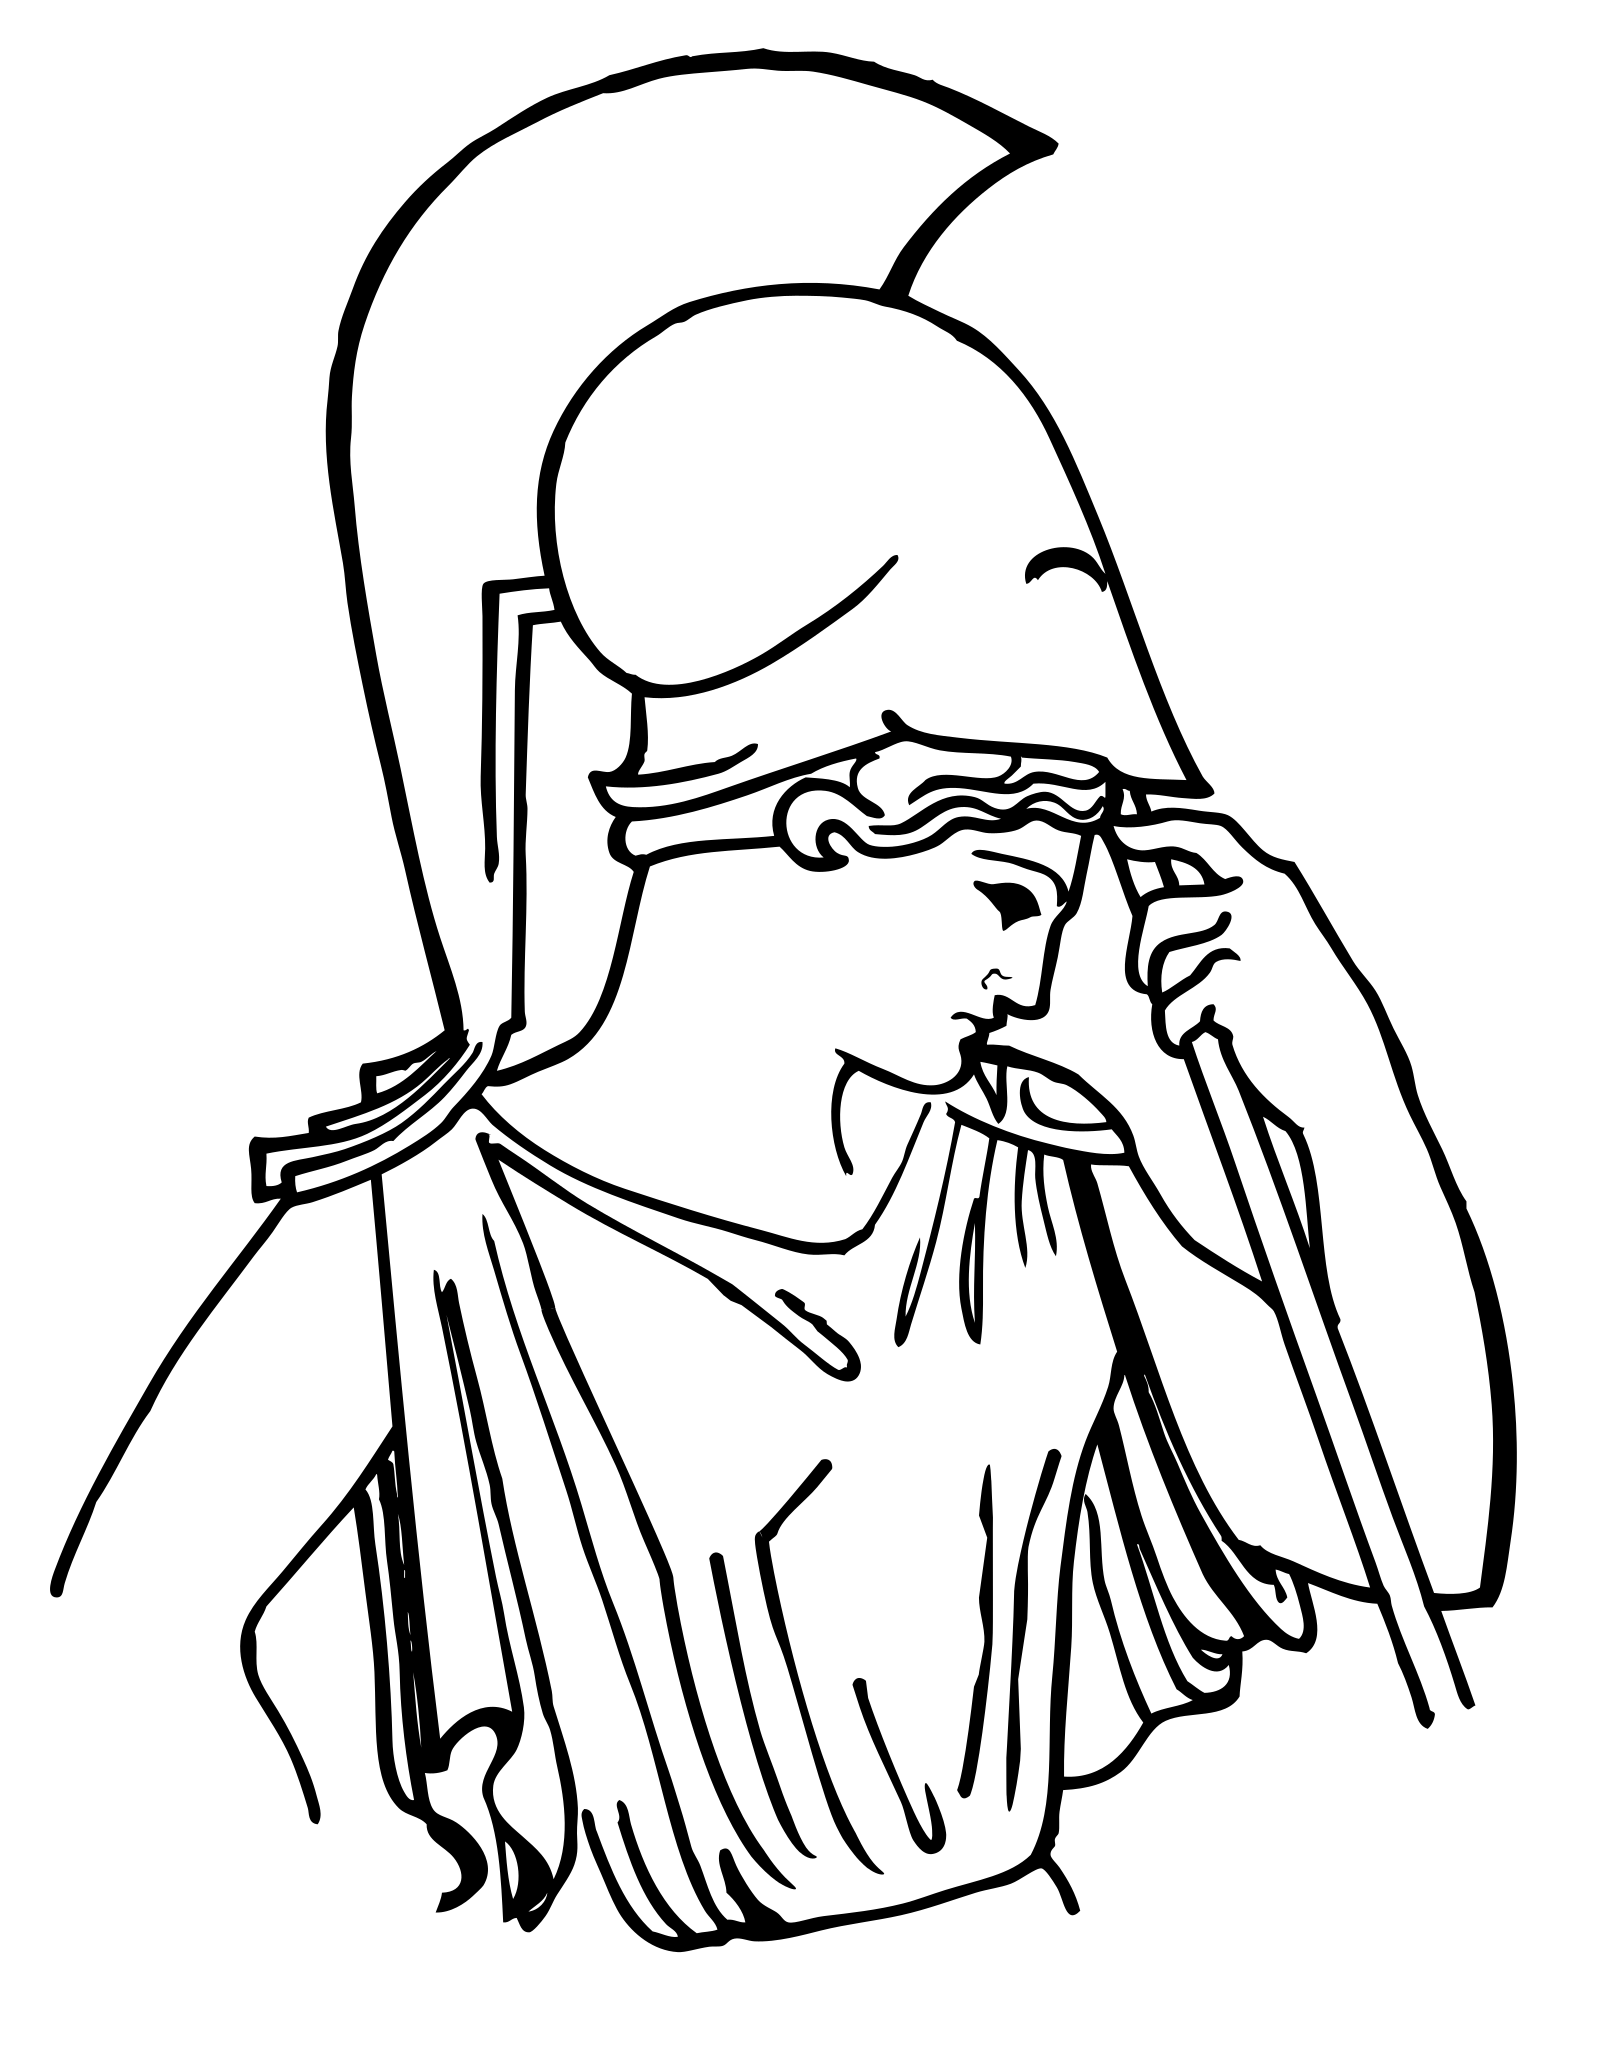
\includegraphics[width=\textwidth]{02}
\vspace{2pt} \\
Efrén Hernández
\vspace*{14pt} \\

\href{https://queridobartleby.es/wp-content/uploads/2021/05/Efren-Hernandez.jpg}{Foto:} \href{Tomada del blog: https://queridobartleby.es/}{Juan Rulfo\textcopyright}
\end{figure}
\vfill
% EPÍGRAFES
\newpage
\pagestyle{empty}
\vspace*{42pt}
\begin{flushright}
\begin{minipage}{7.5cm}
\emph{Efrén Hernández era capaz de orientar rumbos literarios, encender palabras y pensamientos.}
\begin{flushright}
Dolores Castro
\end{flushright}
\vspace*{28pt}
\emph{Efrén parecía un pajarito, pero con unas enormes tijeras de podar me fue quitando toda la hojarasca.}
\begin{flushright}
Juan Rulfo
\end{flushright}
\end{minipage}
\end{flushright}
% CAPÍTULO 1
\chapter[\textsc{Introducción}]{Introducción}\label{ch:introduccion}
\backgroundsetup{
color=black,
scale=2.5, 
hshift=5.7, 
vshift=90,
angle=0,
opacity=.4,
contents=\texttlf{1}
}
\BgThispage
\pagestyle{empty}
\thispagestyle{empty}
\pagestyle{fancy}
\fancyhf{} % Remueve los encabezados y pies previos. Necesario sí o sí.
\fancyhead[CE]{\small\sc el humor como poética en los cuentos de efrén hernández} % Centrados
\fancyhead[CO]{\small\sc 1 \textbullet\ introducción} % Centrados
\fancyhead[RO,LE]{\thepage}
\renewcommand{\headrulewidth}{0pt}
\pagenumbering{arabic}
\setcounter{page}{13}
\section{Semblanza del autor y contexto sociocultural}\label{sec:semblanza-del-autor-y-contexto-sociocultural}
Como cualquier lector inicial de Efrén Hernández, lo primero que conocí de él fue ese breve relato que aparece en diversas antologías del cuento mexicano del siglo \textsc{xx}: ``Tachas'' (1928). Muchos dicen que, al terminar de leerlo, se tiene la sensación de que se trata de un cuento pleno de inocencia y de fino humor, melancólico. No fui la excepción. Tras leer todos sus cuentos reafirmé la idea de estar ante una obra que sutilmente se reía, ``sin aristas hirientes'' como decía Alí Chumacero, de sus personajes, de la trama, del lector, del narrador y aun del autor. Ese rasgo, el humor, me parece que es la parte sustancial de su poética narrativa, su \emph{suma poética}, como intentaré mostrar en este trabajo.

Sobre la vida de Efrén Hernández (León, Guanajuato, 1904-Ciudad de México, 1958) se sabe que a los veintiún años intentó estudiar Derecho en la Escuela Nacional de Jurisprudencia, quizá tratando de emular a su padre, quien fue juez en la ciudad de Guanajuato. No obstante, solo cursó un año por parecerle ``vacío y sin meollo de sustancia verdadera lo que ahí se aprende''.\footnote{Efrén Hernández, ``Ficha autobiográfica'', \emph{Obras} (not. prelim. de Alí Chumacero; recop. de textos de Alí Chumacero y Luis Mario Schneider; bib. de Luis Mario Schneider). Fondo de Cultura Económica, México, 1965, p. 3.} Creía que el conocimiento verdadero residía en ``los hombres de carne y hueso'', en ``los libros buenos'' y en ``el mundo''. Además, su papá había muerto cuando él tenía catorce años y tuvo desde entonces que ganarse la vida por sí mismo.\footnote{\em Ídem.}

Ese desdén hacia la vida universitaria se extendió, asimismo, a los padrinazgos políticos, académicos y culturales, y lo llevó a ejercer los más diversos trabajos para sobrevivir: vendió aretes de plástico, figuritas de yeso, lámparas, libros y productos de la Compañía Nacional de Subsistencias Populares (\textsc{conasupo}); fue archivista y electricista. Antes de llegar a la Ciudad de México había sido aprendiz de botica, de zapatero, de platero y dependiente en una tienda de ropa. Durante su etapa en la capital de la república, recuerda su hija Valentina Hernández Ponzanelli, llegó incluso a hacerse pasar por ``inspector de Salubridad'' en los puestos de comida solicitando una muestra para ``verificar'' su estado cuando el hambre arreciaba.\footnote{Esto me contó el poeta Fernando Rodríguez antes de darme la entrevista donde refería que, en ciertas temporadas, Efrén Hernández vendía aretes de plástico, figuritas de yeso y lámparas para sobrevivir. La entrevista a Fernando Rodríguez (más la de Dolores Castro y Juan Bañuelos) puede consultarse en José Julián González Osorno, ``Efrén Hernández a tres voces'', \emph{Texto Crítico, Nueva Época}, año \textsc{xii}, núm.~24, enero-junio, 2009, pp. 139-145; también en Juan M.~Berdeja y Julián Osorno (coord.), \emph{Mirar no es como ver. Ensayos críticos sobre la obra de Efrén Hernández}. Universidad Autónoma de Querétaro, México, 2018. En un curioso texto donde el hijo de César Garizurieta, el amigo de Efrén que inspiró el personaje de el Tlacuache en ``Tachas'', aclaraba sobre el uso de la expresión ``Vivir fuera del presupuesto es vivir en el error'', se rememoraba sobre este periodo: ``Efrén Hernández, un muy preclaro cuentista mexicano, vivió en su juventud en la colonia de estudiantes aledaña a San Ildefonso. Dada su pobreza extrema subsistía gracias a una credencial de inspector de Salubridad, con la cual iba a los mercados y mediante el típico ``charolazo'' recogía muestras de todo género de abastos que eran analizados sólo por el aparato digestivo del sedicente inspector''. La aclaración sobre la frase de César Garizurieta por parte de su hijo, se puede consultar en \emph{Excélsior} (29 de septiembre, 1995), p. 30-A.} Sus dos empleos mejor pagados quizá fueron el de oficinista en la Secretaría de Educación Pública (\textsc{sep}), junto a Juan Rulfo, y como subdirector de la revista \emph{América}.

Efrén Hernández fue un atento lector de una amplia tradición literaria y filosófica, clásica y moderna.\footnote{Entre estos autores pueden citarse: Cervantes, Santa Teresa, San Juan de la Cruz, fray Luis de León, Quevedo y Góngora; filósofos como Demócrito, Sócrates, Platón, Plotino, Pascal, Nietzsche y Heidegger. Además de don Juan Manuel, Shakespeare, Giono, Gracián, Gómez de la Serna, Hamsun y Faulkner; y textos como \emph{El Panchatantra} y \emph{Las mil y una noches}. Cfr. Marco Antonio Millán, \emph{La invención de sí mismo} (ed. por Daniel González Dueñas y Alejandro Toledo). Consejo Nacional para la Cultura y las Artes, México, 2009, pp. 75 y 81; González Osorno, art. cit.; Federico S.~Inclán, ``Carta a un amigo ausente'', en \emph{América. Revista Antológica, Época Nueva}, núm. 73, sep-oct, 1959, p. 15.} Aunque breve, su obra abarca cuento, poesía, teatro, novela, crítica literaria y dos guiones para cine.\footnote{Sus poemas están contenidos en los libros \emph{Hora de horas} (1936) y \emph{Entre apagados muros} (1943). Las obras de teatro son \emph{Adanijob} (fragmento) y \emph{Cederano}, rescatadas por Alejandro Toledo del archivo de Efrén Hernández y publicadas en \emph{Obras completas} (2012). Sus novelas son \emph{Cerrazón sobre Nicómaco. Ficción harto doliente} (1946), \emph{La paloma, el sótano y la torre} (1949), \emph{Abarca. Fragmento de novela} (1949) y \emph{Autos}, esta última descubierta por Alejandro Toledo entre los papeles de Efrén Hernández y publicada en \emph{Obras completas} (2007). Los ensayos son los comentarios de Efrén acerca de obras de diversos autores, sobre todo mexicanos, contemporáneos a él, la mayoría recopilados por Franco Bagnouls en \emph{Bosquejos} (1995). Alejandro Toledo, ``El guion que Cantinflas no pudo filmar'', \emph{El Universal} (7 de agosto, 2011). \emph{Obras completas} (ed. y prol. de Alejandro Toledo). Fondo de Cultura Económica, México, 2012, p. 5. Véase ``El `Tachas' escribe un asunto para Cantinflas'', \emph{Prensa Gráfica} (21 de mayo, 1949).} Considerados como obras de teatro en las \emph{Obras completas}, \emph{Casi sin rozar el mundo} (1956) fue escrito para María Douglas y \emph{Dichas y desdichas de Nicócles Méndez; tragiburledia cinematográfica} (1951) para Mario Moreno (Cantinflas), esta a petición de Andrés Serra Rojas ---entonces director del Banco Nacional Cinematográfico.

Se creía que el guion para el comediante había sido escrito junto con Dolores Castro, Rosario Castellanos y Marco Antonio Millán; de hecho, se publicó en la revista \emph{América} (núm. 65, abril, 1951) como obra colectiva. No obstante, Castro le aclaró después a Alejandro Toledo ``la invitación a participar en ese proyecto fue un acto de generosidad con dos jóvenes [ella y Rosario Castellanos] que se iniciaban en el mundo de las letras y con Millán, que era su mejor amigo''. El texto se puede acreditar ``casi enteramente a Efrén Hernández''.\footnote{Toledo, art. cit.} Despertó tal entusiasmo esta probable colaboración que en la prensa de la época se decía que el guanajuatense era el guionista que Cantinflas necesitaba.\footnote{``Cantinflas tiene a su alcance el argumentista que necesitaba'', \emph{Ovaciones} (1 de febrero, 1950).}
\section{Till Ealing y la revista \emph{América}}\label{sec:till-ealing-y-la-revista-america}\protect\enlargethispage*{\baselineskip}
Efrén Hernández fue, asimismo, un editor generoso que descubrió e impulsó a importantes escritores. De esto da fe su participación en la revista \emph{América}, a la que ayudó a consolidar dándole un enfoque más literario en su calidad de subdirector.\footnote{Cfr. Lourdes Franco Bagnouls, \emph{Bosquejos} (ed., pról., ns. e índices). Universidad Nacional Autónoma de México"/Instituto de Investigaciones Filológicas"/Centro de Estudios Literarios, México, 1995. [Nueva Biblioteca Mexicana]} Fundada por integrantes de las Juventudes Socialistas Unificadas de México (los poetas Roberto Guzmán Araujo, Manuel Lerín y el ensayista Agustín Rodríguez Ochoa) y de la Juventud Socialista Española, en sus primeros números Alfonso Reyes figuró como miembro de su comité editorial.\footnote{Cfr. Elvira Acuña González, \emph{Índices de \emph{América. Revista Antológica}}. Universidad Iberoamericana, México, 2000, pp. 5-10. [Tesis de licenciatura]} Hernández fue invitado en 1942 por Marco Antonio Millán, el entonces director de la revista, para desempeñarse como editor. Al principio se negó porque le parecía un medio muy político. Finalmente aceptó. Sus primeras participaciones las rubricó como ``Till Ealing''; meses después firmó ya con su nombre. Como subdirector, su presencia fue vital para promover a jóvenes escritores de la época.\footnote{Millán, \emph{op. cit.}, pp. 72-73.}

\emph{América} jugó un papel importante en la vida cultural de México de 1940 a 1969, comparable quizá al que desempeñaron, también en la primera mitad del siglo \textsc{xx}, \emph{Taller}, \emph{Contemporáneos}, \emph{Examen}, \emph{Letras de México}, \emph{El Hijo Pródigo}, \emph{Rueca}, \emph{Pan}, \emph{Dintel}, \emph{Espiral}, \emph{Fuensanta}, \emph{Metáfora}, \emph{Tiras de Colores} o \emph{Estaciones}. Su intención de apoyar a ``gente de letras nueva, valiosa, desconocida o subestimada'' fue un impulso en la difusión de la obra de, entonces, incipientes escritores como Juan Rulfo, Jaime Sabines, Emilio Carballido, Edmundo Valadés, Rosario Castellanos, Juan José Arreola y Dolores Castro, entre otros.\footnote{Rosario Castellanos recuerda de la participación de Efrén Hernández en la revista: ``Durante el tiempo que tuvo a su cargo la dirección de \emph{América} abrió las puertas de par en par a quienes, sin más carta de recomendación que sus manuscritos, se acercaban en busca de un espacio en el cual divulgar [sic] la buena nueva de sus creaciones literarias''. Acuña González, \emph{op. cit.,} p. 20. Véase también Rosario Castellanos, \emph{Obras \textsc{ii}. Poesía, teatro y ensayo} (comp. y ns. Eduardo Mejía). Fondo de Cultura Económica, México, 1998, p. 474. Corchetes míos.} En sus páginas, durante este periodo, se mostró parte de la poesía, la novela, el cuento, el teatro, el ensayo y la crítica del país y de otras naciones latinoamericanas.\protect\enlargethispage*{\baselineskip}

Sobre la importancia de este medio en la promoción de noveles escritores, en 1993 Sergio López Mena había señalado el impulso que esta publicación dio a las primeras creaciones de Rulfo y de otros importantes autores, y el papel destacado que tuvo en ello Efrén Hernández.\footnote{Cfr. Sergio López Mena, \emph{Los caminos de la creación en Juan Rulfo}. Universidad Nacional Autónoma de México, México, 1993, pp. 59-71.} Algunos luego le expresarían su agradecimiento.

Rosario Castellanos, por ejemplo, le decía en una carta de 1942 con timidez:
\begin{quoting}
siento por ustedes [Millán y él] una gratitud muy grande. Han sido tan cordiales, tan amables con nuestros balbuceos. Y recordando que usted es tan bueno y tan sencillo y sabiendo que yo jamás le diría estas cosas personalmente, me atreví a escribírselas.\footnote{En carta fechada en Tehuacán (Puebla), el 25 de septiembre de 1948, Rosario Castellanos agradecía a Efrén Hernández y Marco Antonio Millán el apoyo que le habían dado a ella y a Dolores Castro al publicar sus primeros escritos (\emph{Apuntes para una declaración de fe}, con nota introductoria de Millán) en la revista \emph{América}, además comentaba acerca de sus lecturas y daba su opinión sobre el inicio de la novela \emph{Cerrazón sobre Nicómaco}. Samuel Gordon y Fernando Rodríguez (eds.), ``Cartas de Rosario Castellanos a Efrén Hernández'', \emph{Literatura mexicana \textsc{vii}} (1), 1996, pp. 187-188. Corchetes míos.}
\end{quoting}
Juan Rulfo comentó de él: 
\begin{quoting}
en el archivo de Migración nada se movía porque a nadie le interesaba estar ahí. Con cada cambio de gabinete los corrían a todos, menos a los del archivo del cual ni se acordaban, y en ese departamento donde no sucedía nada nos fuimos a meter Jorge Ferretis y yo, a la sombra de Efrén Hernández. No queríamos que nos viera nadie, para así dedicarnos a nuestras cosas.\footnote{Se ha comentado que Rulfo conoció a Efrén Hernández en 1935 en la Secretaría de Educación Pública (\textsc{sep}) o, quizá, en 1937, en Gobernación (archivo de Migración), donde el guanajuatense fungía como ``jefe''; véase al respecto la entrevista de Elena Poniatowska a Juan Rulfo citada en Roberto García Bonilla, \emph{Un tiempo suspendido. Cronología de la vida y la obra de Juan Rulfo}. Consejo Nacional para la Cultura y las Artes, México, 2008, p. 92.}
\end{quoting}
Ahí Hernández descubrió que el jalisciense escribía a escondidas y luego se deshacía de esos escritos. Intrigado, le solicitó que le mostrara sus cuentos. Quedó asombrado. Tiempo después, en la nota previa al relato ``La cuesta de las comadres'' (\emph{América}, 1948), anotó:
\begin{quoting}
Causa, a un tiempo, de mi más persistente desconcierto y mi mayor confianza, es la manera de rigor, la rigurosísima y tremenda aspiración, el ansia de superación artística de este nato escritor. Cosas que en buena ley son de envidiarse, él, por hallarlas ruines, ha venido rompiéndolas, tirándolas, deshaciéndose de ellas, ¡para volver a hacerlas!

Nadie supiera nada acerca de sus inéditos empeños, si yo no, un día, pienso que por ventura, adivinara en su traza externa algo que lo delataba; y no lo instara hasta con terquedad, primero, a que me confesase su vocación, enseguida a que me mostrara sus trabajos y, a la postre, a no seguir destruyendo.

Sin mí, lo apunto con satisfacción, ``La cuesta de las comadres'', habría ido a parar al cesto.\footnote{Efrén Hernández, ``Presentación a Juan Rulfo, \textquotesingle\textquotesingle{}La cuesta de las comadres\textquotesingle\textquotesingle{}'', \emph{América} (29 de febrero, 1948), núm. 55, \mbox{pp. 31-38.}}
\end{quoting}
Se dice que el guanajuatense ayudó a pulir ciertos aspectos técnicos de la narrativa rulfiana, lo cual es difícil ahora constatar dado que hay poco escrito sobre esto; lo cierto es que Juan Rulfo, en los años finales de su vida, reconoció en él a un maestro: ``a él le debo todo'', dijo en una conferencia.\footnote{Eduardo González Ibarra (Dir.), \emph{Cerrazón sobre Efrén Hernández (documental harto doliente)} (Prod. Enrique Quintero-Mármol; elenc. Dolores Castro, Yanna Hadatty, Alejandro Toledo \emph{et al.}) Canal 22"/Consejo Nacional para la Cultura y las Artes, México, 2016.}

Este apoyo, surgido de la amistad y de la mutua admiración entre estos escritores, ha sido comparado, incluso, con el papel que desempeñó Max Brod con la obra de Kafka.\footnote{Tal como Max Brod hizo con Kafka, apunta Nuria Amat, Hernández rescató a Rulfo del silencio, una generosidad con la palabra de otros escritores que parece hasta insólita en el ámbito literario: ``Lo que hizo en realidad Efrén fue potenciar el estilo personalísimo de su admirado amigo, limpiando ripios, limando retóricas, librándolo de verbosidad y barroquismo y contribuyendo como nadie a un gran salto en la carrera de escritor de Rulfo''. Nuria Amat, \emph{Juan Rulfo, el arte del silencio}. Ediciones Omega, Barcelona, 2003, p. 101. [Vidas Literarias]} En todo caso, Hernández fue para el autor de \emph{Pedro Páramo}, recordaba Arreola, \emph{un alma necesaria y oportuna}.\footnote{Entrevista de Elena Poniatowska citada en García Bonilla, \emph{op. cit.}, p. 113.}

Quizá en gratitud, el jalisciense dio a Hernández para \emph{América} siete de los diecisiete relatos que luego integrarían \emph{El Llano en llamas}: ``Nos han dado la tierra'' (agosto, 1945), ``Macario'' (1946), ``Es que somos muy pobres'' (agosto, 1947), ``La cuesta de las comadres'' (febrero, 1948), ``Talpa'' (enero, 1950), ``El Llano en llamas'' (diciembre, 1950) y ``Diles que no me maten'' (agosto, 1951).\footnote{Además de colaborador en la revista, el jalisciense fue parte del comité directivo. Marco Antonio Millán comentó sobre la publicación paulatina de los cuentos de Rulfo en \emph{América}: ``Juan crecía en tanto le publicábamos poco a poco todo \emph{El Llano en llamas}''. Millán citado en López Mena, \emph{op. cit.}, p. 67.}

Debemos recordar que dos de estos cuentos, ``Nos han dado la tierra'' y ``Macario'', no fueron publicados inicialmente en \emph{América} sino en \emph{Pan}, coordinada por Juan José Arreola y Antonio Alatorre. No obstante, \emph{América} albergó estos siete cuentos antes de formar parte de \emph{El Llano en llamas}, más el relato ``La vida no es muy seria en sus cosas'' (junio, 1945), que no fue incluido en dicho volumen.\footnote{Los cuentos de Rulfo publicados por primera vez en \emph{Pan} son: ``Nos han dado la tierra'', núm. 2, julio, 1945, pp. 1-3; y ``Macario'', núm. 6, noviembre, 1945, pp. 1-3. Los publicados por primera vez en \emph{América}: ``La vida no es muy seria en sus cosas'', núm. 40, 30 de junio, 1945, pp. 35-36; ``Es que somos muy pobres'', núm. 54, 30 de agosto, 1947, pp. 24-29; ``La cuesta de las comadres'', núm. 55, 29 de febrero, 1948, pp. 31-38; ``Talpa'', núm. 62, 29 de febrero, 1948, pp. 79-87; ``El Llano en llamas'', núm. 64, diciembre, 1950, pp. 66-85; y ``Diles que no me maten'', núm. 66, agosto, 1951, pp. 125-130. Cfr. García Bonilla, \emph{op. cit.}, pp. 411-412 y Acuña, \emph{op. cit.}, pp. 174- 175.} Así, con el impulso de estas dos revistas, se iba perfilando y difundiendo, paulatinamente, el magistral libro de Rulfo antes de salir en su primera edición de 1953. Esto fue motivo de enemistad entre el jalisciense y Marco Antonio Millán, director de \emph{América}, dado que le había insinuado la posibilidad de que sus cuentos se publicaran todos, por primera vez, en la revista; finalmente, como se sabe, aparecieron en la colección Lecturas Mexicanas del Fondo de Cultura Económica.

Sería extenso reseñar en este espacio, puesto que cubriría otro tema de investigación, la intensa labor que el guanajuatense tuvo en la promoción de otros escritores y su papel vital en la orientación de nuevos rumbos literarios. Sirva el caso de Rulfo para mostrar hasta qué grado Hernández se llegaba a involucrar como editor, con el solo interés de apoyar a jóvenes escritores de entonces, y para destacar su fino tacto en el descubrimiento de ese tipo de autores que él llamaba ``natos''.
\section{Rasgos generales de su narrativa}\label{sec:rasgos-generales-de-su-narrativa}
Efrén Hernández publicó sus cuentos entre 1928 y 1941, cuando la narrativa mexicana en boga tenía como tema central, o como uno de sus ejes principales, la Revolución mexicana. Sus personajes, anónimos, marginales, distraídos, son soñadores y con frecuencia se demoran en algún circunloquio. Fundada en el humor, esta narrativa es una pluralidad de voces conversacionales que dialogan con ellas mismas, con el autor y con el lector.

Los temas de estos relatos son \emph{inocentes} a simple vista: un clavito que flota en el aire y un escritor que intenta amarrar el tiempo para escribir una historia jamás leída; una Santa Teresa con vida en un cuadro que convive con ratoncitos parlanchines y reflexivos; un pájaro pensante y refunfuñón, un estudiante distraído; un paralítico ansioso de moverse como los árboles; tomates adorados como santos; palabras que caminan, duermen y sueñan... Tras ellos, el guanajuatense plantea, como sin querer, asuntos que dejan perplejos a quienes acompañan su escritura.

Son personajes y temas, evidentemente, alejados de la estética de la Revolución mexicana y de la prosa indigenista de principios del siglo \textsc{xx}; distantes también de la narrativa de Contemporáneos, influida por la vanguardia europea que exploraba poéticamente al sujeto y postergaba la narración. Hay en la narrativa hernandeana, de manera intertextual y como proyección artística, cierto parentesco o afiliación a una tradición visible en obras como \emph{Don Quijote de la Mancha}, donde lo cotidiano, lo pequeño y lo absurdo son algo, al mismo tiempo, maravilloso y trascendente.

Su escritura ha sido vinculada a la vanguardia. Más adelante comentaré sobre esta probable relación, pero anticipo que toda filiación debe partir de la afirmación del propio autor de que su literatura se debía al Siglo de Oro español (``el mejor momento de mi propio y nativo idioma'').\footnote{En el prólogo que escribe para \emph{Liras de amor y muerte} de Roberto Guzmán Araujo, Hernández criticó mordazmente al estridentismo, al surrealismo (cuyos productos eran ``abortos prematuros''), al dadaísmo (incapaz de quitarse su ``tartamudez''), al simbolismo y al academismo. Para él, un escritor debía tener como directrices la originalidad, la sinceridad, la claridad, la sencillez y, sobre todo, debía beber de la tradición literaria propia y no de las corrientes de moda. Véase ``Sobre lo humano en la poesía'' y ``Del surrealismo'' en Franco, \emph{op. cit.}, pp. 33-39, 175-176.} Si compartía con el surrealismo, por ejemplo, que la imaginación era fundamental en la actividad artística, como Breton asentaba en el primer manifiesto surrealista de 1924,\footnote{Cfr. André Breton, \emph{Manifiestos del surrealismo}. Terramar, Buenos Aires, 2006.} o que la poesía era una forma de vida, se distanciaba de él porque no apelaba a un automatismo psíquico en la creación artística ni a un distanciamiento de lo social, tampoco pretendió expresar ``el funcionamiento real del pensamiento''\footnote{\emph{Ibid}., p. 31.} o explorar otros experimentos vanguardistas. La narrativa hernandeana parece nutrirse de una concepción de la literatura donde esta es un referente por sí misma; para él toda obra tenía como fundamento lo humano, así, para desarrollar su poética ficcional, estuvo atento a su realidad y a las voces de su tradición literaria.

De tal modo, ajeno tanto de la narrativa mexicana del \textsc{xx} que transfiguró la historia en tema literario como de la prosa poética de los Contemporáneos, Hernández creó personajes soñadores, distraídos por excelencia, divagadores, pobres; algunos de ellos escritores marginales que se enredan en circunloquios y se lamentan porque el cauce de su escritura se desborda, a menudo, entre las páginas de algún cuento. Hechos de presente, sus pensamientos y diálogos ocurren en el instante. Su ser y su transcurrir están despojados de la gravedad de la historia. Así, para ellos, la adoración de unos tomates puede ser más trascendente que el asesinato del presidente Álvaro Obregón, como se advierte en ``Unos cuantos tomates en una repisita''.\footnote{Las excepciones serían \emph{Abarca} y, en menor grado, \emph{La paloma, el sótano y la torre}, novelas que no son objeto de estudio en este análisis. \emph{Abarca (Fragmento de novela)} trata de la lucha revolucionaria efectuada por Teodoro Abarca contra los federales y está ambientada en el periodo de la Revolución mexicana; fue publicada como ``Abarca (Fragmento de una novela inédita)'' en \emph{América} (núm. 59, febrero, 1949), y póstumamente en las \emph{Obras} de 1965. Por otra parte, \emph{La paloma, el sótano y la torre} (1949), aunque su marco es la Revolución mexicana, la lucha civil no constituye su núcleo narrativo sino el triángulo amoroso entre sus principales personajes: Lina, Fulán y Catito. En la década en que se publicaron las novelas de Efrén Hernández también hay narraciones que se alejan del canon revolucionario, pero que siguen teniendo un claro matiz realista. Entre estas pueden citarse: \emph{Los muros de agua} (1941) de José Revueltas; \emph{La barriada} (1948) de Benigno Corona Rojas; \emph{El sol sale para todos} (1948) de Felipe García Arroyo; \emph{Cabello de elote} (1949) de Mauricio Magdaleno; \emph{Sendas perdidas} (1949) de Mariano Azuela; \emph{La maestrita} (1949) de María Luisa Ocampo; \emph{Río humano} (1949) de Rogelio Barriga Rivas; y \emph{Ojo de agua} (1949) de Rubén Salazar Mallén. Entre los volúmenes de cuentos que ya no tratan el tema revolucionario están \emph{Cinco horas sin corazón} (1940) de Bernardo Ortiz de Montellano; \emph{La noche} (1943) de Francisco Tario; y \emph{Varia invención} (1949) de Juan José Arreola.}
\section{La risa como poética. Propuesta de lectura}\label{sec:la-risa-como-poetica-propuesta-de-lectura}\protect\enlargethispage*{\baselineskip}
Después de leer ``Tachas'' y todo el conjunto de cuentos de Hernández quedó en mí la interrogante de saber qué otorgaba unidad estilística, artística, a esta narrativa. Este trabajo es el intento de respuesta. Estudia las formas y tonos en que se manifiesta el humor en sus cuentos, visto este no como recurso retórico u ornato estético, sino, como señalé, poética narrativa.

Para tal propósito, considero, fundamentalmente, el siguiente \emph{corpus}: ``Tachas'' (1928) y los cuentos incluidos en \emph{El señor de palo} (1932): ``Santa Teresa'', ``Un escritor muy bien agradecido'',\footnote{En la edición de \emph{El señor de palo} (1932) y en la de 1956, \emph{Sus mejores cuentos}, publicada por editorial Novaro, este cuento aparece con el título ``Un gran escritor muy bien agradecido''; en cambio, en las \emph{Obras} de 1965 del Fondo de Cultura Económica y en la más reciente, \emph{Obras completas}, de 2007, se titula ``Un escritor muy bien agradecido''. La variante, ``escritor'' en lugar de ``gran escritor'', no afecta el sentido del cuento, aunque al leerlo es evidente el guiño irónico del autor al usar dicho adjetivo.} ``El señor de palo'', ``Un clavito en el aire''; así como los relatos de \emph{Cuentos} (1941), volumen que sumaba a ``Tachas'' y a los cuentos de \emph{El señor de palo}, ``Incompañía'', ``Sobre causas de títeres'', ``Unos cuantos tomates en una repisita'' y ``Una historia sin brillo''. También los cuatro contenidos en \emph{Obras} (1965): ``Don Juan de las Pitas habla de la humildad'', ``Toñito entre nosotros (estampa)'', ``Trabajos de amor perdidos''\footnote{El título del cuento alude a una de las primeras comedias de Shakespeare: \emph{Love's labours lost}, aunque no hay punto de comparación entre una historia y otra. Hernández publicó ``Trabajos de amor perdidos'' por primera vez en julio de 1941 y, por última, en 1952. En 1941 apareció con el subtítulo ``fragmento de novela'' en \emph{Letras de México}; en junio de 1942 con el título ``A rastras por el suelo'' y con el subtítulo ``fragmento de la novela \emph{Trabajos de amor perdidos}''. Esto hace suponer que Hernández estaba pensando en él como parte de una novela que no concluyó. El héroe de este cuento tiene un aire de familia con Catito, personaje de \emph{La paloma, el sótano y la torre} (1949). En 1952 se fue publicado con el subtítulo de ``fragmento de cuento''. \hyperref[bib:hernandez1952]{Véase Bibliografía}.} y ``Carta tal vez de más''.

La tesis se integra por tres apartados centrales. En el capítulo dos, estudio la irrupción de la vanguardia y su estrecha relación con una risa de ruptura que sacudió las estructuras del cuento, lo cual le imprimió una transformación al género, incluso en Latinoamérica, donde se aprecia claramente ese ``escribir contra la literatura'' que Rafael Lemus vio en Efrén Hernández.\footnote{Rafael Lemus, ``Informe'', en Alejandro Toledo (comp.), \emph{Dos escritores secretos. Ensayos sobre Efrén Hernández y Francisco Tario}. Consejo Nacional para la Cultura y las Artes"/Fondo Editorial Tierra Adentro, México, 2006, p. 42.} Además, analizo la recepción de la obra del escritor guanajuatense entre sus contemporáneos y estudiosos; exploro lo que ha dicho la crítica sobre su posible filiación con la vanguardia literaria hispanoamericana y las apreciaciones de varios autores respecto del humor en ella.

En el capítulo tres indago cómo la perspectiva narrativa de un hombre interior se enlaza al humor y a las constantes digresiones de sus narradores. Este hombre interior, el héroe que suele protagonizar ---y, la mayoría de las veces, narrar---, asume la investidura de algunas figuras clásicas de la risa como el distraído, el niño o el ingenuo, y el paria o marginado, una de cuyas representaciones es el escritor fracasado, variaciones estas del tonto, la figura de la risa por excelencia, como señaló Mijaíl Bajtín en su estudio sobre Rabelais,\footnote{Mijaíl Bajtín, \emph{La cultura popular en la Edad Media y en el Renacimiento. El contexto de Fran"cois Rabelais} (trad. de Julio Forcat y César Conroy). Alianza, Madrid, 1987.} y profundizó Luis Beltrán en \emph{Anatomía de la risa}.

Finalmente, en el cuarto capítulo, exploro algunas formas que adopta la risa en esta cuentística: la relación entre el humor y lo cómico; la intertextualidad con la literatura de la risa y textos clásicos como la Biblia, a menudo desde un punto de vista paródico y desacralizador; el absurdo; el tono conversacional y humorístico hacia el lector, metanarrativo, donde se advierte la plena conciencia de su condición literaria. Debo apuntar que una parte preliminar de este apartado fue publicada en \emph{Mirar no es como ver. Ensayos críticos sobre la obra de Efrén Hernández} con el título de ``Diálogos intertextuales en la cuentística de Efrén Hernández''.

En suma, en este trabajo estudio el papel de la risa en la configuración de los cuentos del guanajuatense, la cual, se intenta demostrar, es fundamental en la visión del mundo desde la que se escribe, no como recurso retórico sino como poética ficcional, es decir, la forma y proyección artística como se relatan los cuentos, la forma como se configura su discurso, las temáticas y personajes. A través de la risa el autor disuelve los grandes discursos (la historia, entre ellos), los trastoca, los subvierte, y configura narraciones donde se privilegia lo nimio, lo intrascendente, lo cotidiano.
\cleardoublepage
% EPIGRAFE
\newpage
\pagestyle{empty}
\vspace*{42pt}
\begin{flushright}
\begin{minipage}{7.5cm}
\emph{La pugna de Efrén Hernández no es contra la literatura mexicana sino contra la literatura. Contra la trama. Contra el sentido. Contra el lenguaje. Contra todo aquello que impide decir la vida amorfa.}
\begin{flushright}
Rafael Lemus
\end{flushright}
\end{minipage}
\end{flushright}
% CAPÍTULO 2
\chapter[\textsc{Risa, vanguardia y cuento hispanoamericano}]{Risa, vanguardia y cuento hispanoamericano}\label{ch:risa-vanguardia-y-cuento-hispanoamericano}
\backgroundsetup{
color=black,
scale=2.5, 
hshift=5.7, 
vshift=90,
angle=0,
opacity=.4,
contents=\texttlf{2}
}
\BgThispage
\thispagestyle{empty}
\pagestyle{fancy}
\fancyhf{} % Remueve los encabezados y pies previos. Necesario sí o sí.
\fancyhead[CE]{\small\sc el humor como poética en los cuentos de efrén hernández} % Centrados
\fancyhead[CO]{\small\sc 2 \textbullet\ risa, vanguardia y cuento hispanoamericano} % Centrados
\fancyhead[RO,LE]{\thepage}
\renewcommand{\headrulewidth}{0pt}
\pagenumbering{arabic}
\setcounter{page}{27}
\section{Manifestaciones de la risa vanguardista}\label{sec:manifestaciones-de-la-risa-vanguardista}
La vanguardia, señala Saúl Yurkievich, ``instaura la ruptura de la tradición y la tradición de la ruptura''.\footnote{Saúl Yurkievich, ``Los avatares de la vanguardia''. \emph{Revista iberoamericana}, 1982, vol. 48, núm. 118, p. 351.} La razón es que los movimientos artísticos que componen la vanguardia (el cubismo, el futurismo, el expresionismo, el imaginismo, el dadaísmo, el ultraísmo y el surrealismo) resultan de una crisis y, en su afán de superarla, buscan romper radicalmente con el pasado. Por eso se trata de rupturas que aspiran a renovaciones profundas en el arte, a la transformación absoluta.\footnote{\em Ídem.}

Esa revolución se ancla, sobre todo, en un cuestionamiento de la racionalidad capitalista, de la ética y sentido del arte heredados de la sociedad decimonónica burguesa. Por eso la vanguardia acoge con alegría la ofensa al buen gusto burgués de los decadentistas y los simbolistas, y se orienta a la producción de nuevos símbolos culturales. La vanguardia, apunta Hugo Achugar, es
\begin{quoting}
un tipo de producción simbólica que disolvió definitivamente ciertas concepciones heredadas de la segura sociedad decimonónicamente burguesa, al proponer el relativismo de toda producción artística y
filosófica como algo propio de una civilización que sabía o había aprendido la historicidad de todo lo construido por el hombre y su eventual caducidad. En cierto modo podría afirmarse que la vanguardia muestra la modificación, o mejor aún, la creación de un nuevo imaginario social.\footnote{Hugo Achugar, ``El museo de la vanguardia: para una antología de la narrativa vanguardista hispanoamericana'', en Hugo J.~Verani (ed.), \emph{Narrativa vanguardista hispanoamericana}. Universidad Nacional Autónoma de México, México, 1996, p. 13.}
\end{quoting}
En este nuevo imaginario social, que toma fuerza principalmente en el París de finales del \textsc{xix}, el escenario hasta entonces reconocido como propio de la actividad artística cambia. Como asienta Bolívar Echeverría, la figura del artista se desplaza de los talleres de arte institucionales a cafés y cabarés, en los que ``la vida se libera de su compulsión productivista'' y se acerca al mundo de la fiesta, lo cual simboliza la vuelta del arte a su matriz premoderna.\footnote{Bolívar Echeverría, ``De la academia a la bohemia y más allá''. \emph{Theoría. Revista del Colegio de Filosofía}, núm. 19 (2009), p. 51. [En línea:] \url{http://ru.ffyl.unam.mx/bitstream/handle/10391/853/06_Theoria_19_Echeverria_49-62.pdf?sequence=1&isAllowed=y} [Consulta: 5 de agosto, 2022]} A partir de este desplazamiento, el arte de vanguardia deja atrás la \emph{mímesis de la realidad} y se resuelve en una \emph{mímesis festiva}, que es
\begin{quoting}
una mímesis de segundo grado, que no imita la realidad sino la desrealización festiva de la realidad; una mímesis que no retrata los objetos del mundo de la vida sino la transfiguración por la que ellos
pasan cuando se encuentran incluidos en otra mímesis, aquella que la existencia festiva hace del momento extraordinario del modo de ser humano.\footnote{\emph{Ibid.}, p. 55.}
\end{quoting}
La fiesta es una interrupción del modo ordinario de la vida humana, y una de sus señas es la irrupción de un caos lúdico vinculado a la risa. Es como si en la fiesta ``el caos ---lo otro, humanizado o `domesticado' como la contraparte del cosmos humano--- hiciera un gesto de amenaza,
fingiera hacer estallar esa humanización o `domesticación', destruirla (así sea, lúdicamente, para reconstruirla después)''.\footnote{\emph{Ibid.}, p. 53.} En esta destrucción de la fiesta, la risa es la gran protagonista.

El mundo en que nacieron las vanguardias, el de los cafés y cabarés, no es el de la fiesta popular masiva, de épocas anteriores a la modernidad, como el carnaval medieval, pero conserva parte de su
esencia y no se disuelve por completo en la privatización o el individualismo del tiempo de ocio.\footnote{Luis Beltrán anota que ``En Occidente, la fiesta semanal se ha convertido en el fin de semana, de momento de dos días. Y aún se le añaden los periodos de vacaciones. El resultado es la pérdida del sentido alegre de la fiesta y de la comunidad feliz. La fiesta deja de ser el tiempo de la alegría, de la risa, para convertirse en el tiempo del ocio, un tiempo sin actividad productiva, un tiempo para el aislamiento''. Luis Beltrán Almería, \emph{Anatomía de la risa}. Ediciones Sin Nombre"/Consejo Nacional de Ciencia y Tecnología"/ Universidad de Sonora, México, 2011, p. 19. [Relámpago la risa; coord. Martha Elena Munguía Zatarain]} La vida de los cafés y cabarés, pese a estar inscrita en el tiempo del ocio, es un cronotopo festivo en el que surge, aunque restringido, el ambiente de la fiesta universal, sobre todo a través de la ingesta de alcohol. Sus participantes, como los de la gran fiesta universal, también experimentan una liberación transitoria a través de la que acceden al ``reino utópico [...] de la libertad, de la igualdad y de la abundancia''.\footnote{Mijaíl Bajtín, \emph{La cultura popular en la Edad Media y en el Renacimiento. El contexto de Fran"cois Rabelais} (trad. Julio Forcat y César Conroy). Alianza, Madrid, 1987, p. 15.}

El historiador francés Georges Minois comenta sobre ese ambiente a través de la figura del borrachín en los cafés franceses de fines del siglo \textsc{xix}: ``se revuelca en el lodo, apesta, vomita, escupe, orina, se pee. Su apestoso talante pertenece a la muy popular boga de la suciedad que amenizaba los cafés-concierto, o a los lectores del \emph{Journal des merdeux}''.\footnote{El \emph{Journal des merdeux} (trad. al español como \emph{Diario de mierda}) fue una publicación finisecular de un único número editada en 1882 por Jules Jouy (1855-1897). Georges Minois, \emph{Historia de la risa y la burla: del Renacimiento a nuestros días}. Universidad Veracruzana"/Ficticia"/Consejo Nacional de Ciencia y Tecnología, México, 2018, p. 290.}

El borrachín es la encarnación del caos lúdico que surge en la fiesta, de ahí su fuerza nihilista, destructiva. ¿Podemos dudar de que el borrachín es imagen del caos festivo, que, como señala Echeverría, es la pantomima de una amenaza que se dirige a la domesticación humana y finge destruirla?

En ese París finisecular que evoca Minois, el arte no solo estaba impulsado por la risa insensata y descabellada, también por un humor oscuro y desencantado representado por Georges Courteline (1859-1929). Ambos talantes, sin embargo, partían de un punto común enraizado en el espíritu de los tiempos: ``el sentimiento del sinsentido del universo y el carácter indeterminado, indecidible, de las cosas''.\footnote{\emph{Ibid.}, p. 358.} En honor a este sentimiento es que ``entre la depresión y la fantasía, el hombre de fines de siglo flota, sin puntos de referencia, riéndose de todo y de nada [...]''.\footnote{\em Ídem.} Fue esta risa insensata, descabellada, oscura, hija del sinsentido, la que hizo del París de la Bella Época la capital de la risa y de la vanguardia, pues esta heredó de aquella su fuerza nihilista, caótica y destructiva.

Son incontables las veces en que la ruptura de la tradición que instauró la vanguardia se dio a través de la risa, como podemos apreciar en ``Dadá manifiesto sobre el amor débil y el amor amargo'' de Tristan Tzara (\mbox{1896-1963}), que es una suerte de irónicas instrucciones ``para hacer un poema dadaísta'', de una risa cuyo objetivo es la tradición y, en un giro de auto-escarnecimiento, del propio movimiento Dadá.\footnote{Tristan Tzara, \emph{Siete manifiestos Dadá}. Tusquets, México, 2013, p. 50.}
\section[¿Un escritor de vanguardia u original?]{"?Un escritor de vanguardia u original?}\label{sec:un-escritor-de-vanguardia-u-original}
La narrativa de Efrén Hernández ha sido ligada a la vanguardia iberoamericana de los años veinte y principios de los treinta. Esta tesis fue sugerida por John Brushwood, para quien el autor guanajuatense es un escritor moderno porque ``va desde los experimentos de la época vanguardista hasta la reafirmación de las mismas tendencias en la nueva novela''.\footnote{John Brushwood, ``Efrén Hernández y la innovación narrativa''. \emph{Nuevo Texto Crítico}, año \textsc{i}, núm. 1, (primer semestre, 1988), p. 93.}\protect\enlargethispage*{\baselineskip}

En 1995 Franco Bagnouls señaló la aparente paradoja respecto de esta filiación: ``¿por qué [Efrén Hernández] parece criticar en sus artículos ciertas formas de lo literario [vanguardistas] que se dan en la narrativa escrita por él?''.\footnote{Lourdes Franco Bagnouls, \emph{Bosquejos} (ed., pról., ns. e índices). Universidad Nacional Autónoma de México"/Instituto de Investigaciones Filológicas"/Centro de Estudios Literarios, México, 1995, p. 25. [Nueva Biblioteca Mexicana]} La posible similitud, según Franco, puede entenderse a la luz de ``una nueva estética presidida por la ruptura con la realidad tangible e inmediata en busca de nuevas formas de asociación''.\footnote{\emph{Ibid.}, p. 26.} En esta búsqueda, la exploración de los mecanismos del inconsciente era importante pero no determinante.

También Hugo J.~Verani y Fernando Burgos consideraron a Efrén Hernández en sus antologías sobre narrativa vanguardista.\footnote{Verani incluye a Hernández, como representante de la vanguardia hispanoamericana, al lado de Roberto Arlt, Macedonio Fernández, Oliverio Girondo, Pablo Palacio, Vicente Huidobro, Pablo Neruda, Martín Adán, César Vallejo, Felisberto Hernández, Julio Garmendia, Salvador Novo, Arqueles Vela y Gilberto Owen. El estudio-antología contiene ``Tachas'' como uno de los cuentos mexicanos representativos de esta estética. Burgos selecciona ``Un clavito en el aire'' como cuento representativo de Hernández de la estética vanguardista. Hugo J.~Verani (ed.), \emph{Narrativa vanguardista hispanoamericana}. Universidad Nacional Autónoma de México, México, 1996. Fernando Burgos (introd. y ns.), \emph{El cuento hispanoamericano en el
siglo \textsc{xx}}. Castalia, Madrid, 1997.} Asimismo, Yanna Hadatty señaló que hay en su obra temprana rasgos del dadaísmo, del surrealismo, cubismo y del expresionismo; destacó además la importancia que tiene el uso del símil en sus cuentos, lo cual, desde la perspectiva de la investigadora, lo acerca a los recursos retóricos utilizados por los vanguardistas.\footnote{Yanna Hadatty Mora, \emph{Autofagia y narración. Estrategias de representación en la narrativa iberoamericana de vanguardia, 1922-1935}. Iberoamericana Vervuet, Madrid, 2003, pp. 96-97.}

Por otra parte, Elizabeth Hochberg destacó en la narrativa hernandeana un rasgo considerado propio de estos movimientos artísticos: la clara intencionalidad de interrelacionar las artes. Esto puede advertirse, señala, en ``El señor de palo'', donde algunos elementos dan cuenta de esas posibilidades representativas del arte verbal frente a la imagen visual. Además en varios textos del escritor guanajuatense pueden advertirse narradores que usan estrategias pictóricas para representar el mundo exterior, descripciones y referencias al arte visual: ``Podemos asociar esta presencia de representaciones artísticas dentro de la narrativa [de Hernández] con la écfrasis''.\footnote{Hochberg también ha estudiado el vínculo existente entre la narrativa de Efrén Hernández, la de los Contemporáneos y los estridentistas, dado el interés común de estos escritores por las relaciones entre la literatura y el arte visual. En Hernández, señala, destaca el interés de sus narradores por la pintura, la fotografía, la escultura y la artesanía, ``para describir, nombrar o aludir a formas que ya son representaciones artísticas''. Elizabeth Hochberg, ``Más que `pálidas sombras': nuevas posibilidades ecfrásticas en la narrativa de Efrén Hernández''. \emph{Perífrasis}, vol. 4, núm. 7, enero-junio, 2013, p. 71; Elizabeth Hochberg, \emph{La écfrasis en los cuentos de Efrén Hernández} (Dir. Sergio López Mena). Universidad Nacional Autónoma de México, México, 2012 [Tesis de maestría] [En línea]: \url{http://132.248.9.195/pmig2019/0690721/Index.html} [Consulta: 5 de agosto, 2022] y Elizabeth Hochberg, ``Efrén Hernández y las preocupaciones interartísticas de la vanguardia mexicana''. \emph{Revista Liberia 1}, 2013, p. 4. [En línea]: \url{https://revistaliberia.files.wordpress.com/2013/05/hochberg.pdf} [Consulta: 5 de agosto, 2022]}

Críticos como Esperanza López Parada y Rafael Lemus afirman que se trata de un autor inclasificable, un \emph{outsider}, un marginal. Un novelista distinto entre los distintos, por ser su escritura descentrada y rebasar los géneros.\footnote{Esperanza López Parada, \emph{Una mirada al sesgo. Literatura hispanoamericana desde los márgenes}. Iberoamericana Vervuert, Madrid"/Frankfurt, 1999, pp. 11-12.} Escritura que semeja el camino que traza la silla de ruedas de ``El señor de palo'': \emph{no sigue la línea recta de la narrativa tradicional, pues, como una raíz o un rizoma, transita por líneas alternativas}.\footnote{\emph{Ibid.}, p. 12. Cursivas mías.}

Rafael Lemus anota sobre esta excentricidad, vale la pena citarlo en extenso por su planteamiento:\protect\enlargethispage*{\baselineskip}
\begin{quoting}
Se dice: es raro porque es secreto. Porque se opone al cauce principal, realista, de la literatura mexicana. Porque no es Juan Rulfo o Carlos Fuentes. Se repasa su obra ---una novela, dos docenas de
relatos, una obra teatral, algunos poemas--- como para despacharla apresuradamente. Para decir: sí, es rara. Para apuntar: no, no es \emph{La sombra del caudillo} o \emph{La tumba}. Quien así procede ---así proceden casi todos--- no comprende lo esencial. Esto: la pugna de Efrén Hernández no es contra la literatura mexicana sino contra la literatura. Contra la trama. Contra el sentido. Contra el lenguaje. Contra todo aquello que impide decir la vida amorfa. Por eso hay que leerlo fuera de su contexto inmediato. Hay que decir: Efrén Hernández es mexicano, y otra cosa. Decir: es un autor mayor, a veces enorme, y leerlo al lado de otros autores mayores, a veces enormes. Leerlo, sobre todo, para entender el cómo. ¿Cómo se impide fijar? ¿Cómo pronuncian aquí y allá lo informe? Leerlo para descubrir un método. Una escritura de lo informe.\footnote{Rafael Lemus, ``Informe'', en Alejandro Toledo (comp.), \emph{Dos escritores secretos. Ensayos sobre Efrén Hernández y Francisco Tario}. Consejo Nacional para la Cultura y las Artes"/Fondo Editorial Tierra Adentro, México, 2006, pp. 42-43.}
\end{quoting}
López Parada y Lemus coinciden en que Hernández no sigue el modelo mimético realista (aristotélico); su obra es propia de una literatura posmoderna: fragmentaria, digresiva, que niega la discursividad grandilocuente.

En suma, lectores y críticos han visto en él a un escritor autobiográfico, \emph{sui generis}, que rompe con las formas de narrar realistas, un escritor vanguardista, a pesar suyo, en cuya escritura, me parece, la risa tiene un papel fundamental.
\section{Cuentistas hispanoamericanos de vanguardia}\label{sec:cuentistas-hispanoamericanos-de-vanguardia}
En su \emph{Antología crítica del cuento hispanoamericano del siglo \textsc{xx} (1920-1980)}, José Miguel Oviedo señala que la vanguardia en Hispanoamérica tiene un desarrollo ``autónomo, divergente y profundamente creador'', en el que se involucran ``fuerzas propias que exceden, estética y cronológicamente, las propuestas originales de la vanguardia''.\footnote{José Miguel Oviedo, \emph{Antología crítica del cuento hispanoamericano del siglo \textsc{xx} (1920-1980). \textsc{i}. Fundadores e innovadores}. Alianza, Madrid, 2002, p. 13.} Un claro ejemplo es el creacionismo del poeta chileno Vicente Huidobro, cuyos presupuestos teóricos se asientan en el manifiesto \emph{Non serviam}, de 1914, y al que da una forma más acabada en 1916, poco antes de viajar a Europa. El caso del creacionismo permite lanzar la idea, señala Oviedo, de que ``la literatura de vanguardia no se desplaza en un solo sentido a través del Atlántico, es un vaivén; mejor aún: una red que se abre en múltiples direcciones interconectadas''.\footnote{\em Ídem.} Otro ejemplo es el del surrealismo, que si bien nace en Francia, se arraiga en Hispanoamérica con características, alcances y propuestas propias.

Jorge Schwartz sostiene que se puede considerar a \emph{Non serviam} (1914) como el punto de arranque de las vanguardias en América Latina: ``Tanto por la actitud cuanto por los irreverentes postulados, \emph{Non serviam} representa el momento inaugural de las vanguardias del continente''.\footnote{Jorge Schwartz, \emph{Las vanguardias latinoamericanas}. Fondo de Cultura Económica, México, 2006, p. 37.} Su declive comienza a verse después de 1938, año del encuentro en México entre Diego Rivera, León Trotsky y André Breton y de la escritura conjunta del ``Manifiesto por un Arte Revolucionario Independiente'', que, señala Schwartz, ``es importante por su influencia en la toma de posición política de los artistas europeos de vanguardia y sus repercusiones en América Latina'',\footnote{\emph{Ibid.}, p. 40.} esto en relación a que reclamaba: ``la independencia del arte-por la revolución; la revolución-por la liberación definitiva del arte''.\footnote{André Breton, León Trotski \emph{et al.}, \emph{Manifiesto por un arte revolucionario independiente}. Siglo \textsc{xxi}, México, 2019, p. 44.}

En el prólogo a \emph{Narrativa vanguardista hispanoamericana}, Hugo Achugar señala que los textos fundamentales de la vanguardia hispanoamericana pueden encontrarse en la segunda y tercera décadas del siglo \textsc{xx}.\footnote{Cuando el proceso de expansión del capitalismo se vería interrumpido por la Primera Guerra Mundial (1914-1918), y el colapso de la Bolsa de Valores de Wall Street (1929), que llevaría a una crisis económica global.} En la selección de Achugar y Verani se incluyen narraciones publicadas entre 1922 y 1932 por Roberto Artl y Macedonio Fernández (Argentina); Vicente Huidobro (Chile); Pablo Palacio (Ecuador); Martín Adán y César Vallejo (Perú); Efrén Hernández, Salvador Novo, Gilberto Owen y Arqueles Vela (México);\footnote{Aunque Vela nació en Guatemala, la mayor parte de su vida se desarrolló en México.} Felisberto Hernández (Uruguay) y Julio Garmendia (Venezuela). A decir de Achugar, estos autores
\begin{quoting}
propusieron un nuevo modo imaginario de entender y representar la vida cotidiana, tanto a nivel individual como social, a la vez que explotaron (¿explosionaron?) los fundamentos estéticos y artísticos heredados. Es decir, se apartaron de una concepción de una narrativa para proponer otra que negaba, hasta cierto punto, una tradición con larga vigencia.\footnote{Achugar, art. cit., p. 16.}
\end{quoting}
La lista de los cuentistas de vanguardia se enriquece con las incorporaciones que hace Fernando Burgos a \emph{El cuento hispanoamericano en el siglo \textsc{xx}}: el guatemalteco Rafael Arévalo Martínez; los chilenos María Luisa Bombal, Juan Emar y Héctor Barreto; el argentino Ricardo Güiraldes y el mexicano Julio Torri.\footnote{Cfr. Burgos, \emph{op. cit.}, p. 15.} En \emph{Voces recobradas. Narrativa mexicana fuera del canon (\mbox{1925-1950})}, Lourdes Franco Bagnouls agrega a José Martínez Sotomayor, María Ramona Rey, Alberto Quintero Álvarez, César Garizurieta, Luis G.~Basurto, Solón de Mel y Rubén Salazar Mallén.\footnote{El verdadero nombre de Solón de Mel era Guillermo de Luzuriaga y Bribiesca (Ciudad de México, 1895-1959). Fundó y dirigió revistas como \emph{El trovador}, \emph{Alma Bohemia} y \emph{Alma Latina}, también fue redactor de \emph{El Universal Ilustrado}. Cfr. Lourdes Franco Bagnouls, \emph{Voces recobradas. Narrativa mexicana fuera del canon (1925-1950)}. Universidad Nacional Autónoma de México, México, 2008, p. 386.}

Sin duda, estudios recientes van dando cuenta ya de más descubrimientos y el número deba ser mayor, pero, más que realizar una lista exhaustiva de los cuentistas de vanguardia, debe reconocerse su presencia y no pasarse por alto, algo común en las historias de la literatura hispanoamericana, que se enfocan principalmente en el regionalismo y el modernismo. Como señala Hugo J.~Verani: ``la presencia de una narrativa contestataria y de ruptura, que privilegia el libre ejercicio de la imaginación, fue más abundante y considerable de lo que suelen reconocer las historias de la literatura hispanoamericana.\footnote{Hugo J.~Verani, ``La narrativa hispanoamericana de vanguardia'', en Hugo J.~Verani (ed.), \emph{Narrativa vanguardista hispanoamericana}. Universidad Nacional Autónoma de México, México, 1996, pp. 41-42.}
\section[Características del cuento vanguardista]{Características del cuento vanguardista hispanoamericano y el papel de la risa}\label{sec:caracteristicas-del-cuento-vanguardista-hispanoamericano-y-el-papel-de-la-risa}\protect\enlargethispage*{\baselineskip}
Achugar destaca ocho características fundamentales de la narrativa vanguardista, especialmente del cuento:
\begin{enumerate}[noitemsep]
\item La ``invasión de la primera persona'', es decir, los relatos son narrados por un ``yo'' que no es el sujeto sólido y de una pieza de los cuentos de épocas y tendencias artísticas anteriores, sino un personaje discontinuo y fragmentado;
\item el desmantelamiento de los fundamentos lógicos de la narrativa realista; esto dio como resultado relatos que no siguen las coordenadas espacio-temporales o las leyes de causa-efecto tradicionales y se abren a mundos oníricos;
\item el impacto de la revolución psicológica y tecnológica en la creación de personajes y espacios;
\item una importante influencia de la poesía en la escritura;
\item preferencia por personajes degradados o marginales;
\item la consciencia metadiscursiva y metanarrativa;
\item el espacio ficcional predominantemente urbano; y
\item la presencia destacada de la risa.\footnote{Cfr. Achugar, art. cit., pp. 23-30.}
\end{enumerate}
A decir de Hugo Achugar, la transformación narrativa de la prosa vanguardista se debe a la invasión de la primera persona;\footnote{Achugar, art. cit., p. 23.} de ahí que, como señala Franco Bagnouls, el proceso narrativo se decanta hacia los procesos mentales y emocionales del propio narrador: 
\begin{quoting}
La esencia del cuento vanguardista radica en su estructura. El discurso transcurre por vías inusuales que obedecen más a los procesos de la mente que a los hechos concretos. El principal interlocutor es el propio emisor del discurso, que encuentra en el monólogo interior la vía idónea de comunicación.\footnote{Franco, \emph{Voces...}, p. 46.}
\end{quoting}
Si Efrén Hernández es el paradigma de esta invasión, otro mexicano, César Garizurieta, tiene un estilo muy parecido, en el que el interior y el exterior forman un continuo determinado por la subjetividad, léase, por ejemplo, ``Pobre gato''.\footnote{César Garizurieta, ``Pobre gato'' citado en Franco, \emph{Voces...}, p. 416.}

En un estilo diferente, la importancia de los procesos mentales, el rol protagónico del \emph{yo}, también está presente en los cuentos del uruguayo Felisberto Hernández, como en ``El vapor'', donde se aprecia la \emph{invasión de la primera persona}: ``Y sin darme cuenta caí en la impersonalidad: parecía que todo el cuerpo se me hubiera salido por los ojos''.\footnote{Felisberto Hernández, ``El vapor'', en \emph{La cara de Ana}, Edición Dominio Público, 1930. [En línea]: \url{http://www.creativecommons.uy/wp-content/uploads/2015/01/Felisberto-Hernandez-La-cara-de-Ana.pdf} [Consulta: 5 de agosto, 2022]}

Esta \emph{invasión de la primera persona} representa un desplazamiento del foco del relato del mundo exterior al mundo interior, a la subjetividad. El protagonismo de muchos de estos relatos recae por completo en esa interioridad fragmentada en un cúmulo de vivencias, al grado de que, según Franco: ``el cuento vanguardista carece de interacción; cuando en él hay un `Tú', este se deslíe hasta convertirse en una mera evocación, en un sustrato cuyo papel se limita a ser el detonante de los procesos mentales del narrador''.\footnote{Franco, \emph{Voces...}, p. 37.} Es el caso del ya mencionado ``Pobre gato'' de César Garizurieta, donde se presenta a un narrador fragmentario y discontinuo, lejano del confiable narrador de la cuentística anterior.

Achugar lo caracteriza como ``ese yo, o sujeto en primera persona, que poetiza la narración no es una construcción sólida y consistente''.\footnote{Achugar, art. cit., p. 24.} Su resquebrajamiento se alía con la dislocación de las coordenadas espacio-temporales y la ruptura de las leyes de causa-efecto tradicionales como una manera de romper y cuestionar la racionalidad burguesa, característico en el cuento vanguardista.\footnote{\emph{Ibid.}, pp. 23-24.}

Franco señala respecto de esta ruptura: ``El cuento vanguardista impone su propio orden y a él se somete más allá de la lógica que impone la realidad''.\footnote{\emph{Ibid.}, p. 46.} ``El difunto y yo'', de Garmendia, es una clara muestra de esto, pero también ``Pobre gato'', de Garizurieta, pues el narrador despliega una parte del relato como un sueño y desde la perspectiva de un gato, con lo que logra un efecto de desdoblamiento que choca con nuestra racionalidad. El cuento muestra el estrecho vínculo entre el derrumbe de los principios lógicos que rigen la realidad y la apertura al mundo onírico, un mundo tan fragmentario como el \emph{yo} que toma la batuta en los relatos de vanguardia.

Otro ejemplo de apertura al mundo onírico es ``El unicornio'', de Juan Emar, donde encontramos estampas como la siguiente: ``Golpearon a la puerta. Entró una dama anciana. Entre sus manos traía un pedazo de arcilla en el que se hallaba enterrado, por el tacón, un viejo zapato de mujer conteniendo un verso de Espronceda''.\footnote{Juan Emar, \emph{Diez}. Ercilla, Santiago, 1937, p. 94.} Se trata, sin duda, de una estampa surrealista, el movimiento de vanguardia que acogió con mayor generosidad la lógica onírica.

La recuperación del espacio onírico está muy ligado a su carácter intimista: ``El acontecer de un cuento intimista se sujeta al tiempo flexible de la ensoñación antes que al tiempo de los aconteceres. El espacio no pasa de ser muchas veces un mero decorado; lo esencial es el sujeto que narra su experiencia íntima y por ello el espacio está dentro de él y lo contiene''.\footnote{Franco, \emph{Voces...}, p. 36.} Es importante recordar que el psicoanálisis contribuyó a la fragmentación del sujeto a través de la noción del inconsciente y tuvo un impacto artístico en la vanguardia. Esta disciplina fragmentó al sujeto consciente y racional, para revelarnos a un habitante de mundos inconscientes y pletórico de energías oníricas. Paralelamente, la vanguardia configuró narradores fragmentados que se mueven con soltura en esos mundos y que, incluso, hacen guiños al psicoanálisis, como se dice en ``Pobre gato'':
\begin{quoting}
Quizás debiera hablar del subconsciente, pero en caso de que yo me atreviera a hablar de Adler o Yung, usted pondría el dedo en la llaga de su boca roja, en señal de silencio para que no citara autores, así es que no hablaré, se lo prometo, del subconsciente y mucho menos del fenómeno onírico.\footnote{\emph{Ibid.}, p. 417.}
\end{quoting}
El cuento de vanguardia muestra además la influencia de la revolución tecnológica en el mundo narrado;\footnote{Como señala Hugo Achugar: ``La transformación de la vida cotidiana debida a la
revolución tecnológica implica una nueva percepción de la naturaleza o del entorno...'', Achugar, art. cit., p. 24.} también en ``Pobre gato'' encontramos asociaciones de ese tipo: ``Siempre el pequeño héroe que abrigamos dentro del corazón niño: salvar una rosa que pretende deshojar el viento, rescatar a la mujer amada del dragón que trae una instalación eléctrica en sus fauces, o bien ayudar al pobre grillo telegrafista''.\footnote{Franco, \emph{Voces...}, p. 416.}

Así como la vanguardia asimiló los fenómenos de la revolución tecnológica, también encontró en la poesía, cuya afinidad al uso de la primera persona es de sobra conocida, una manera de expresarse.\footnote{\emph{Ibid.}, p. 36.} Los cuentos de Efrén Hernández, como veremos más adelante, son un buen ejemplo de esta apertura a la palabra poética, que él conduce con maestría hacia el humor en la confección de lo que Alcántara llama metáforas-bromas.\footnote{Juan Francisco Javier de Alcántara Pohls, \emph{Efrén Hernández y los problemas de la imaginación}. Universidad Iberoamericana, México, 1993, p. 368. [Tesis de Licenciatura]}

Otra característica del cuento vanguardista es el protagonismo de los seres degradados o marginales.\footnote{Cfr. Achugar, art. cit., p. 26.} Así son, por ejemplo, los personajes de \emph{Un hombre muerto a puntapiés} de Pablo Palacio, pederastas, antropófagos, impotentes y brujas, entre otros. En otros relatos, como en los del mismo Efrén Hernández, el foco se centra en personajes pobres, aniñados, tontos o locos que develan un mundo distinto al ordinario. Ejemplos de ello se hallan asimismo en ``El coleccionista de ruidos'', de Solón de Mel, donde el protagonista es un esquizofrénico, ``el Loco de los Ruidos''.\footnote{Franco, \emph{Voces...}, p. 387.}

Vemos aquí el interés de la vanguardia por los elementos desconcertantes y anómalos de la realidad, o lo que Oviedo llama ``la zona oscura de la experiencia personal: los estados parapsicológicos y la percepción extrasensorial, las perturbadoras visiones del sueño y la comunicación telepática''\footnote{Oviedo, \emph{op. cit.}, p. 21.} que rigen la estructura onírica, el tono lírico y a los personajes de contextura larval que participan de estos relatos.\footnote{\em Ídem.}

El grupo de personajes degradados y marginales del cuento de vanguardia se completa con otros que tienen conciencia de su naturaleza ficticia. Aunque esta conciencia metadiscursiva y metanarrativa es un rasgo del relato vanguardista, tiene raíces ``en el pasado secular de la narrativa occidental (Cervantes, Sterne)'',\footnote{Achugar, art. cit., p. 27.} que es retomado por Macedonio Fernández, Pablo Palacio, Julio Garmendia y Efrén Hernández.

La conciencia metadiscursiva y metanarrativa no se expresa únicamente en los personajes, sino también en los ``juegos lingüísticos que llaman la atención a las características fundamentales del lenguaje
y referencias a la creación de la obra que estamos leyendo'',\footnote{Brushwood, art. cit., p. 87.} como los que Brushwood encuentra en Macedonio Fernández y Efrén Hernández y que, a su parecer, abren la puerta a las reflexiones sobre la metaficción en los relatos de ambos.

La apertura a la metaficción del relato vanguardista amplía el espacio de la ficción a ``la propia página en blanco donde se registra la palabra'',\footnote{Achugar, art. cit., p. 29.} por lo que el espacio ficticio de la vanguardia, que también se ha ampliado con la introducción de mundos oníricos, es múltiple y predominantemente urbano.\footnote{\em Ídem.}

Finalmente, y como es notable en ``El cuento ficticio'', los relatos metaficcionales abrazan la risa como un componente importante. Como hemos visto, la risa es un elemento fundamental de la vanguardia, ``una de las manifestaciones de la desacralización de lo literario''.\footnote{\emph{Ibid.}, p. 31.} Un claro ejemplo es ``El pájaro verde'', de Juan Emar, que no solo evoca las andanzas en la bohemia parisina del chileno, sino que ``es la reescritura paródica del cuento \textquotesingle\textquotesingle Un corazón simple\textquotesingle\textquotesingle\ (\textquotesingle\textquotesingle Un c\oe ur simple\textquotesingle\textquotesingle) de Gustave Flaubert'',\footnote{Soledad Traverso, ```Pájaro verde' de Juan Emar: Un manifiesto vanguardista''. \emph{Acta literaria}, 2001, núm. 26, p. 155.} una parodia que ``puede leerse como un manifiesto vanguardista en contra del arte como copia de la realidad, para adherir a un arte no representacional y autónomo''.\footnote{\em Ídem.} Del mismo Emar se puede mencionar ``El unicornio'', donde un hombre, muy distraído, pone en todos los periódicos de su ciudad un aviso para recuperar su personalidad porque se le ha perdido.\footnote{Emar, \emph{op. cit.}, p. 91.}

También en Macedonio Fernández está presente esta risa. En su caso, es parte imprescindible de un proyecto metafísico que, contra la metafísica occidental, se centra en la nada y en la ausencia: ``Es la misión de hacer presente la Nada la que le da un lugar central a la humorística dentro de la empresa mística de Macedonio de pasar de una metafísica de la presencia a una metafísica de la ausencia''.\footnote{Nicolás Rojas Sierra, ``Humor y misterio en Macedonio Fernández: \emph{Los Papeles de Recienvenido}''. \emph{Literatura: teoría, historia, crítica}, núm. 12, octubre, 2010, pp. 71-98.} Fernández logra esto a través del absurdo que habita tanto en el conocido chiste: ``Fueron tantos los que faltaron que si falta uno más, no cabe'', como en diálogos tan disparatados como los de \emph{Papeles de Recienvenido}.\footnote{Macedonio Fernández, \emph{Papeles de Recienvenido y Continuación de la Nada, Obras completas}, vol. 4. Buenos Aires, Corregidor, 2004, p. 23.} La misma lógica absurda de alcances metafísicos se encuentra en ``El zapallo que se volvió cosmos'', donde un fruto de dimensiones pantagruelescas engulle al mismo Ser.\footnote{Macedonio Fernández, \emph{Relato, cuentos, poemas y misceláneas, Obras completas}, vol. 8. Buenos Aires, Corregidor, 2004, p. 54.}

La risa vanguardista tiene esa carga subversiva que se vuelve, sobre todo, contra la misma literatura, y si bien, como señala Achugar, la vanguardia hispanoamericana no tiene el estruendo de los movimientos europeos, sí está marcada por ``una relativización del carácter sagrado de la literatura''.\footnote{Achugar, art. cit., p. 32.} Se trata de una risa orientada a concebir de una nueva manera la obra literaria, a su desacralización mediante la risa; la vanguardia representó la ruptura definitiva con las formas artísticas del siglo precedente.\footnote{Franco, \emph{Voces...}, p. 36.}

Resulta imposible abarcar completa la estrecha relación entre la risa y las vanguardias en este apartado. Solo resta anotar que esa relación no debe obviarse en el estudio del cuento hispanoamericano y mexicano de vanguardia, pues, como veremos enseguida, esta risa de carga destructiva, a veces nihilista, constituye uno de sus rasgos más característicos. Es a través de su revisión que podremos apreciar la obra de Efrén Hernández en su justa dimensión; aunque el propio autor se desmarcó de los ``vanguardismos'', hay en ellos un elemento fundamental para los fines de este trabajo que los une: la risa en sus producciones literarias.
\cleardoublepage
% EPÍGRAFE
\newpage
\pagestyle{empty}
\vspace*{42pt}
\begin{flushright}
\begin{minipage}{7.5cm} % 7.5 cm (defecto)
\emph{Verdaderamente volamos. Nuestro núcleo es de alas. Nuestro operar se iguala al de los sueños. La vida es una fábula, un cambiante fructificar sueños. Nunca sabremos nada. Sólo, sí, que asistimos en forma inaprehensible al escenario mágico de un manantial de cuentos.}
\begin{flushright}
Efrén Hernández \\ ``Dos líneas sobre el cuento''
\end{flushright}
\end{minipage}
\end{flushright}
% CAPÍTULO 3
\chapter[\textsc{Figuras de la risa en la cuentística de Hernández}]{Figuras de la risa en la \\ cuentística de Hernández}\label{ch:figuras-de-la-risa-en-la-cuentistica-de-hernandez}
\backgroundsetup{
color=black,
scale=2.5, 
hshift=5.7, 
vshift=90,
angle=0,
opacity=.4,
contents=\texttlf{3}
}
\BgThispage
\thispagestyle{empty}
\pagestyle{fancy}
\fancyhf{} % Remueve los encabezados y pies previos. Necesario sí o sí.
\fancyhead[CE]{\small\sc el humor como poética en los cuentos de efrén hernández} % Centrados
\fancyhead[CO]{\small\sc 3 \textbullet\ figuras de la risa en la cuentística de hernández} % Centrados
\fancyhead[RO,LE]{\thepage}
\renewcommand{\headrulewidth}{0pt}
\pagenumbering{arabic}
\setcounter{page}{45}
\section{Sentidos del reír: lo nimio}\label{sec:sentidos-del-reir-lo-nimio}
En los cuentos del escritor guanajuatense la perspectiva cotidiana del mundo es puesta en suspenso a través del humor. La risa, unida a una visión del mundo crítica, sirve al autor para trastocar los grandes discursos y cincelar una narrativa donde se privilegia lo nimio, lo intrascendente.

Octavio Paz fue de los primeros en advertir esta relación al considerar a Hernández de prosa ``divagatoria y como escrita en una vigilia que ya el sueño empieza a inundar'', heredero del linaje de Micrós.\footnote{Octavio Paz, ``Efrén Hernández, \emph{Entre apagados muros}'', en \emph{Miscelánea \textsc{i}. Primeros escritos}, t. \textsc{xiii}. Fondo de Cultura Económica, México, 1998, p. 307.} Apreciación semejante tuvo Alí Chumacero al apuntar que Hernández y Micrós eran escritores que ``suelen descubrir en la palpitación de lo nimio, en la pequeñez de la vida cotidiana, el temblor de la existencia''.\footnote{Alí Chumacero, ``Nota preliminar'', en  \emph{Obras} (not. prelim. de Alí Chumacero; recop. de textos de Alí Chumacero y Luis Mario Schneider; bib. de Luis Mario Schneider). Fondo de Cultura Económica, México, 1965, p. \textsc{vii}. Ver también Alí Chumacero, \emph{Los momentos críticos}. Fondo de Cultura Económica, México, 1996, 1"a ri., p. 267.} Destacó el aspecto autobiográfico de esta narrativa:
\begin{quoting}
Acaso nadie, en las letras mexicanas de los últimos lustros, haya redactado sus textos con tal semejanza consigo mismo, con tanto amor por su íntimo impulso afectivo. Mucho contribuyó a reforzar esa actitud la fidelidad a lo autobiográfico. Las experiencias inmediatas, el recuerdo de las pasadas, la sospecha de las venideras, aparecen a tramos transformadas en minuciosas observaciones.\footnote{\em Ídem.}
\end{quoting}
Pero este rasgo personal está unido a la capacidad del escritor de trasladar una visión del mundo pícara y sutilmente maliciosa a una literatura en la que los propios pensamientos del autor son víctimas de una risa burlona.\footnote{Valentina, la hija de Efrén Hernández, señaló sobre el sentido del humor de su padre: ``Escribir sobre ese hombre que fue Efrén Hernández, la verdad me resulta bastante difícil, pues mi padre aún ahora me parece tan cercano que me cuesta mucho trabajo afocarlo con claridad, y por otro lado siento que han pasado tantos años desde que se ausentó, que los recuerdos me llegan muy nebulosos. Unas veces veo su rostro con una nitidez que casi me asusta, sus ojos vivaces tras los lentes de gruesos cristales que no lograban ocultar la vitalidad y constante asombro ante todo lo que le rodeaba, y aquel destello picaresco muy propio de una persona con un increíble sentido del humor''. ``Lo que mi padre nunca contuvo fue su especial buen humor como su inagotable ingenio para hacer bromas''. Efrén Hernández, \emph{Obras completas} (ed. y pról. Alejandro Toledo). Fondo de Cultura Económica, México, vol. 2, 2012, pp. 518-519.} Al parecer de Chumacero, Hernández era como Catito --- personaje de \emph{La paloma, el sótano y la torre} (1949)---:
\begin{quoting}
Me conocía harto pícaro y harto mosca muerta y mátalas callando --- dice [Catito]---, y precisamente en estas malas propiedades basaba mi satisfacción, y en estas dotes, en rigor negativas, ponía toda mi complacencia. Eso era de niño, y de persona mayor tales premisas, fundadas en la destreza de sus expresiones literarias, le allanaron el camino para hacer burla aun de sus propios pensamientos.\footnote{\emph{Ibid.}, p. \textsc{viii}. Efrén Hernández, \emph{La paloma, el sótano y la torre}. Secretaría de Educación Pública, México, 1949, p. 12. Corchetes míos.}
\end{quoting}
El autoescarnio al que alude Chumacero, tal vez una virtud primordial del humor, fue asimismo destacado por Rosario Castellanos en los personajes de Hernández, verdaderos \emph{desadaptados, marginales y cándidos}.
\begin{quoting}
El habitante del universo de Efrén es un inocente. No adquiere nunca un empaque de seriedad, no se hace responsable de lo que le rodea, no se adapta a las circunstancias y, menos aún, las domina; no
triunfa sobre los otros. Inerme, vaga por habitaciones ruinosas o por solitarias calles nocturnas. Es pobre, como conviene a su falta de sentido práctico; es desdeñado, como cuadra a su falta de agresividad y de orgullo, a su significancia social. Pero si no inspira respeto tampoco solicita nuestra compasión ni despierta nuestra burla. Porque está lleno de una malicia finísima, porque él se
adelanta a reírse de sí mismo, primero, y luego de nosotros.\footnote{Rosario Castellanos, ``La obra de Efrén Hernández'', en \emph{Mujer de palabras. Artículos rescatados de Rosario Castellanos} (comp., intro. y ns. de Andrea Reyes). Consejo Nacional para la Cultura y las Artes, México,
2004, p. 191.}
\end{quoting}
La minucia en la observación vista por Chumacero y esta risa acentuada por una ``malicia finísima'' señalada por Castellanos son apreciaciones del registro característico de los cuentos hernandeanos, donde priva una risa sutil que, para mayor elegancia, aparece en una narrativa sobre el pensamiento.

Así lo hace notar también Edmundo Valadés, para quien el sutil humorismo de los personajes hernandeanos no puede separarse del ejercicio de la razón, la imaginación y la contemplación, únicos lujos que pueden permitirse estos en medio del aislamiento y la pobreza en los que su autor los inserta:
\begin{quoting}
Aunque queda en duda si Efrén se propuso sus relatos para hacer reflexiones o si usó de sus reflexiones para hacer relatos, él es la inocencia. No son la acción ni las pasiones las que mueven a esos personajes, sino el ejercicio de la razón, por medio de una lógica de sutiles humorismos, para tratar de explicarse, desde la inmovilidad física, y casi siempre en el aislamiento de un humilde cuarto, las mínimas incidencias propias o las del mundo exterior. De allí partirán a su viaje imaginativo, la contemplación de los objetos o imágenes que están cerca.\footnote{Edmundo Valadés, ``Efrén Hernández o de la inocencia'', en \emph{México en el arte}, núm. 11 (1985"/1986), p. 10.}
\end{quoting}
Valadés consideró a Hernández como un heredero de la literatura de la risa castellana, en su vertiente clásica, la de los Siglos de Oro español, pero no reconoce en él el poder destructivo de la sátira que la caracteriza, y matiza: ``si, en diversos tránsitos de su prosa escribió bajo esa influencia, al fin lo hizo con la malicia purificada de malas intenciones: el humorismo que no hiere ni agrede, sino que incita una sonrisa benévola''.\footnote{\em Ídem.}

Porque, en realidad, el objetivo de Hernández no era sancionar mediante la risa sino redescubrir el mundo a través de los detalles minúsculos que escapan a nuestra conciencia cotidiana desde el humor. Dice Valadés: 
\begin{quoting}
Efrén o sus personajes reflexionan como si el mundo acabara de ser descubierto precisamente en sus zonas menos advertidas ---en eso pequeño que no solo rodea a tantos seres humildes o pobres, sino que puede ser para ellos lo más importante y decisivo---, pero con una suave ironía, que podría ser burla juguetona al trascendentalismo, al tremendismo.\footnote{\emph{Ibid.}, p. 11.}
\end{quoting}
Y es que el linaje realista del tremendismo es ajeno a los mundos ficcionales de Hernández.\footnote{Con gran acierto Juan Berdeja ha observado la necesidad de estudiar a esos escritores marginales, raros, que privilegiaban lo nimio, y en apariencia intrascendente, en medio de una estética inspirada en la gran gesta revolucionaria y en los sucesos alrededor de ella. Fijar la atención justo no en ese mural artístico emanado de la Revolución sino en la grandeza de lo cotidiano, donde se revela la búsqueda de lo total en lo diminuto y en lo pueril, volver los ojos a lo \emph{microscópico}, a los \emph{pequeños cosmos}: ``Hernández muestra caras del mundo que no podríamos apreciar sin su literatura: su mirada que tiende hacia lo mínimo muestra los puntos que unen al orbe diegético en elementos diminutos que van cobrando relevancia. [...]; todos son objetos que llevan a los protagonistas a entender que su mundo es el de la correspondencia, donde todo, por más insignificante que parezca, contiene en sí al universo''. Juan M. Berdeja, ``El ojo microscópico: la relevancia de lo nimio y lo mínimo en el arte narrativo, pictórico y guiñol posrevolucionario'', en \emph{Cuadernos de Literatura}, vol. 23, núm. 43, enero-julio, 2018, p. 155. [En línea]: \url{https://revistas.javeriana.edu.co/index.php/cualit/article/view/23043/20160} [Consulta: 8 de agosto, 2022]}

Cabe destacar que Valadés calificó los tonos de la risa hernandeana sin \emph{aristas hirientes}: los relatos de Hernández son ``de una gracia gentil y agudamente reflexiva sobre mínimos pormenores; la de humorismo sin aristas hirientes; la visión de un mundo leve que tiene el don de la sonrisa [...]''.\footnote{Valadés, art. cit., p. 11.} Emmanuel Carballo también destacó de ellos este ``humorismo depurado''.\footnote{Emmanuel Carballo, ``Efrén Hernández, el cuentista más extraño del siglo \textsc{xx}''. \emph{El Universal} (24 de febrero, 2004).}

Por su combinación entre humorismo y sentido del absurdo, anota John Brushwood, Efrén guarda similitudes con Macedonio Fernández, en la medida en que ambos ``expresan ideas serias, sobre el conflicto realidad"/irrealidad y sobre las posibilidades expresivas, en un contexto siempre ameno, humorístico y frecuentemente absurdo''.\footnote{John Brushwood, ``Efrén Hernández y la innovación narrativa'', en \emph{Nuevo Texto Crítico}, año \textsc{i}, núm. 1, (primer semestre, 1988), p. 87.} Un absurdo, como se lee en ``Tachas'', inherente a la realidad: ``Lo natural sería, dice Gómez de la Serna, que los pajaritos dormidos se cayeran de los árboles. Y todos lo sabemos bien, aunque es absurdo, los pajaritos no se caen''.\footnote{Efrén Hernández, \emph{Tachas} (epílogo de Salvador Novo). Secretaría de Educación Publica, México, 1928.} Para Brushwood, Efrén Hernández ``proyecta una visión profunda del problema realidad"/irrealidad sin perder la \emph{habilidad de burlarse de sus propios pensamientos}''.\footnote{Brushwood, art. cit., pp. 93-94. Cursivas mías.}

Alcántara Pohls destacó la importancia del juego y la broma en la escritura hernandeana, así como su relación con una perspectiva del mundo infantil: ``Si jugar y bromear son actos infantiles y maliciosos, si embuste y juguetes son equivalentes, si la mentira y la fantasía son necesarias para embaucar, entonces la literatura, la escritura, tal y como las concibe Efrén Hernández, son actos infantiles''.\footnote{Juan Francisco Javier de Alcántara Pohls, \emph{Efrén Hernández y los problemas de la imaginación}. Universidad Iberoamericana, México, 1993, pp. 24-25. [Tesis de Licenciatura]} Según su perspectiva, este autor inscribe su arte en el ámbito lúdico: 
\begin{quoting}
Escribir es jugar y bromear. Al menos así sucede en gran parte de sus cuentos, los cuales muchas veces no tienen un argumento o está reducido al mínimo, y sólo consisten en una serie de digresiones desorientadoras, juegos de imaginación y bromas maliciosas.\footnote{\emph{Ibid.}, p. 25.}
\end{quoting}
Este aspecto ``infantil'' se relaciona con el impulso lúdico que atraviesa esta narrativa, el cual convive con una mezcla de ironía y amargura, de humorismo y tristeza.\footnote{\emph{Ibid.}, p. 26.} Para Alcántara, este elemento lúdico, estas \mbox{metáforas-broma}, se manifiestan en toda la cuentística del escritor, en su lenguaje y en la lógica con que se proyecta la narración:
\begin{quoting}
A lo largo de los cuentos no escapan tampoco las palabras, el lenguaje mismo, la lógica: todo puede ser objeto de juegos, material para una broma. Abundan los enredos con refranes populares, las analogías caprichosas, las personificaciones de objetos o animales, las animalizaciones de personas, los falsos razonamientos, las bromas al lector, los detalles chuscos, los nombres cómicos o ridículos, las ensoñaciones sobre palabras, las falsas etimologías, e incluso un género particular de metáforas que son características de Efrén Hernández: las metáforas-bromas.\footnote{\emph{Ibid.}, p. 25.}
\end{quoting}
Como ejemplo de este original sistema, Alcántara menciona la siguiente metáfora-broma presente en ``El señor de palo'': ``Al aire, parece que lo tenían de las orejas y que si se moviera se las estirarían''.\footnote{\em Ídem.} En los capítulos siguientes volveré a referirme a estas reflexiones, pues el objetivo de este apartado solamente es dar un panorama general de las lecturas de la risa en los cuentos de Hernández.

Franco también señaló la presencia del humor en esta escritura. En \emph{Bosquejos} anota sobre los ensayos del guanajuatense, apreciación que bien puede extenderse a su cuentística:
\begin{quoting}
Efrén Hernández usa con frecuencia recursos bergsonianos para desencadenar la risa. Bergson habla de esos pequeñísimos resortes de índole muy diversa que van desde las actitudes corporales hasta la semántica de la palabra, pasando por la sintaxis; producen el efecto del muñeco de alambre que salta intempestivamente de una caja de sorpresas y causa hilaridad por lo inesperado de la situación, por la fractura en el tono mantenido y porque rompe con la norma. Este factor sorpresa se puede dar de manera única e irrepetible, pero puede darse también como reacción en cadena o reiterativamente. Efrén Hernández utiliza este recurso; rompe, con términos coloquiales o con diminutivos, periodos en los que la atención se acerca a límites de peligrosidad; o, por el contrario, estos muñecos de resortes son puntillas que acentúan más la ironía del texto.\footnote{Lourdes Franco Bagnouls, \emph{Bosquejos} (ed., pról., ns. e índices). Universidad Nacional Autónoma de México"/Instituto de Investigaciones Filológicas"/Centro de Estudios Literarios, México, 1995, pp. 17-18. [Nueva Biblioteca Mexicana]}
\end{quoting}
Franco advierte que el ingenio ---a través de inesperadas comparaciones, por ejemplo--- es otro factor de ruptura que Hernández usa para conducir a sus lectores al terreno de la risa, la cual, tanto en sus cuentos como en sus ensayos, abre un territorio de complicidad en el que aparece con naturalidad y fluidez el diálogo con el lector y la reflexión personal: ``En este fluir de lo cómico, la prosa de Efrén Hernández se adelgaza en un discurso convertido en charla, con su dosis de complicidad correspondiente. Es diálogo con el lector y reflexión personal''.\footnote{\emph{Ibid.}, p. 18.}

Este diálogo y reflexión va unido al humor, destacó Ana García Bergua en el prólogo a \emph{Tachas y otros cuentos}, donde señala la importancia de los acontecimientos de la conciencia en ``Tachas'', equiparable a la de los acontecimientos del mundo narrado:
\begin{quoting}
Entonces lo más notable de ``Tachas'' es la claridad con que Efrén Hernández asume aquel ``soltar las riendas'', que le llevará a elaborar relatos de gran complejidad en los que la realidad de los pensamientos, recuerdos e imaginaciones del narrador y los personajes corre pareja con la trama de lo que se cuenta, en una especie de trastocamiento del orden de las prioridades que no es nada ajeno al humor.\footnote{Ana García Bergua, ``Prólogo'' a \emph{Tachas y otros cuentos}. Universidad Nacional
Autónoma de México, México, 2002, p. 13.}
\end{quoting}
Tal apreciación es importante para comprender el papel de la risa en la cuentística de Hernández: la igualdad entre los acontecimientos de la conciencia y los de la trama, mediada por el humor, resulta en un trastocamiento, una alteración del orden y las jerarquías del mundo ordinario.

Esta alteración se extiende al plano axiológico, en la medida en que el \emph{alter ego} que el escritor introduce en sus cuentos, ese personaje que en el universo de la ficción da cuenta de la perspectiva del mundo del autor, tiene una fuerte conciencia de su superioridad moral:
\begin{quoting}
Ya fuera por una idea moral o por un complejo, ciertamente el \emph{alter ego} de Efrén Hernández en sus cuentos establece una diferencia con los otros: yo soy así, dice, y a veces por ser así sale perdiendo de manera trágica o amarga; sin embargo, hay detrás de él la sonrisa maliciosa del que se sabe superior a los otros, y que no pierde por no saber lo que debe hacer, sino porque no quiere hacerlo.\footnote{\emph{Ibid.}, pp. 15-16.}
\end{quoting}
Nuevamente encontramos una caracterización de la risa hernandeana como la sonrisa maliciosa de quien se sabe superior. Pero esta no debe confundirse con la risa del satírico, presta para condenar y castigar desde su superioridad moral. La risa de Hernández se aleja de ella en la medida en que es atravesada, como ya habían reparado Chumacero y Castellanos, por la autoburla, el autoescarnio. Anota García que las figuras ficcionalizadas del autor que aparecen en su cuentística encarnan una
\begin{quoting}
Voluntad que sería pueril si no entrañara, antes que nada, una idea estética. Y que, para colmo de superioridades, se sabe reír de esta puerilidad: ``Tengo mucho miedo de morir sin haber llegado a desengañar al mundo de que mi genio es, en realidad, de una profundidad extraordinaria. Tú lo verás'', dice el narrador de ``Un clavito en el aire'', y ya no sabemos si habla en serio o se burla de nosotros.\footnote{\emph{Ibid.}, p. 16.}
\end{quoting}
A veces este humor se enlaza al absurdo y la ironía:
\begin{quoting}
De la combinación de estos dos elementos (el absurdo y el humor) arranca probablemente toda la narrativa de Hernández: hablar de lo absurdo como si fuera natural o convertir lo irreal en posible. El humor, entonces, actúa como tamiz por su efecto siempre distanciador de la realidad: lo más absurdo presentado jocosamente nos lo parecerá menos. Pero el principio contrario no es menos cierto, e innumerables veces nos acercaremos a través de su mirada irónica a lo que de inverosímil y extraordinario encierra la cotidianidad.\footnote{María del Mar Paúl Arranz, ``Efrén Hernández o el juego cómplice de la literatura'', en \emph{Literatura Mexicana}, vol. 5, núm. 1, 1994, p. 94. [En línea]: \url{https://revistas-filologicas.unam.mx/literatura-mexicana/index.php/lm/article/download/1088/1060} [Consulta: 9 de agosto, 2022]}
\end{quoting}
Es la capacidad de Hernández de convertir lo irreal en posible a través de la risa, del absurdo, del humor, de la ironía, lo que lo acerca a las vanguardias, como señala Fernando Rodríguez: ``Con un sentido del humor que pocos tienen en la literatura mexicana. Un humor trágico, en ocasiones surrealista, aunque él no estuviera a favor del surrealismo''.\footnote{José Julián González Osorno, ``Efrén Hernández a tres voces'', en \emph{Texto Crítico, Nueva Época}, año \textsc{xii}, núm. 24, enero-junio, 2009, p. 145.} Cierto que Hernández se asumía lejano de las vanguardias, pero su cuentística tiene ciertos elementos comunes con este movimiento artístico, como ya mencioné. Es el caso del absurdo, que cuando aparece lo hace sin el amargo talante existencialista que asfixia a los personajes de Beckett, como observó Rafael Lemus.\footnote{Rafael Lemus, ``Informe'', en Alejandro Toledo (comp.), \emph{Dos escritores secretos. Ensayos sobre Efrén Hernández y Francisco Tario}. Consejo Nacional para la Cultura y las Artes"/Fondo Editorial Tierra Adentro, México, núm. 117-118, 2006, pp. 67-68.}

La risa de esta narrativa es más una sonrisa, pero no aquella amarga del que conoce el absurdo de la existencia, sino la del ingenuo que se enfrenta a las cosas como si fuera la primera vez, con asombro. El absurdo de estos cuentos, como señala Martha Munguía, es, más bien, una plena ruptura con la lógica ordinaria.\footnote{Martha Elena Munguía Zatarain, \emph{La risa en la literatura mexicana: apuntes de poética}. Iberoamericana Vervuert"/Bonilla Artigas, 2012, p. 158.} Esta narrativa devela el absurdo del orden cotidiano porque
\begin{quoting}
Sus cuentos están habitados invariablemente por personajes extraños, que parecen mirar las cosas por primera vez, que se detienen a analizar, a desmenuzar para tratar de penetrar en el misterio que se encierra en cada objeto familiar, en cada palabra insulsa que se pronuncia; en este detenerse se revela como absurda la lógica que siempre hemos tenido por racional y cuerda, como ajeno y estrafalario lo que ha sido valorado como normal y natural.\footnote{\em Ídem.}
\end{quoting}
En esta cuentística, enfatiza Munguía, la risa puede tomar la mano del dolor, puede manar de las mismas desgracias de los personajes, pero también del absurdo, de las incoherencias y de la agudeza con que observan el mundo desplegado ante ellos con la ingenuidad del niño, incluso del tonto.\footnote{\emph{Ibid.}, pp. 159-160.} Parece que en estas historias no ocurre nada y nada se cuenta; sin embargo, en ellas la aventura de la imaginación y del pensamiento desenmascara mentiras y devela absurdos:
\begin{quoting}
Los cuentos de Efrén Hernández no parecen contar nada, no hay héroes, no hay grandes aventuras, como no sea la de la imaginación, la de la persecución obstinada de un razonamiento, la de una sutil respuesta desenmascaradora de la mentira, del absurdo de lo usual. Por eso sus personajes son ``anormales'', distraídos, ensimismados, negados a dejar atrás la infancia. Es un punto de enunciación el que sostienen, el que les permite establecer las conexiones inesperadas entre las ideas, entre las palabras, entre los objetos y la relación de éstos con la vida. Estamos aquí muy lejos de los tonos satíricos admonitorios o de la risa estridente de la burla; asistimos al nacimiento de un sutil, apenas insinuado, sentido del humor que religa el arte verbal con el juego y restablece así el verdadero y profundo sentido de contar una historia.\footnote{\emph{Ibid.}, p. 160.}
\end{quoting}
A través de estos personajes ``anormales'', apunta Munguía, se muestra el absurdo del mundo y se desenmascaran las mentiras con un humor sutil, lúdico, con el que parece retomarse el núcleo mismo del cuento.

Este tono de los cuentos vincula al autor guanajuatense con una rica tradición literaria de la risa, sobre todo con la del Siglo de Oro español. Edmundo Valadés había señalado que en la obra de Hernández hay ``ecos de las letras del Siglo de Oro''. Sobre todo, apunta por su parte Juan M. Berdeja, del humor de Cervantes a través de la figura de Sancho Panza: ``divertido sabio que encuentra, al igual que Hernández, su materia discursiva en el dicho popular y la ironía''.\footnote{Juan Manuel Berdeja Acevedo, \emph{Efrén Hernández o el arte de la digresión}. Universidad de Guanajuato"/Ediciones del Lirio, México, 2019, p. 40. [Arte y Literatura]} Según Berdeja: ``no se puede negar que el espacio de Hernández es el margen [...]: se coloca entre la seriedad de los sentimientos que representan y provocan sus personajes y el humor de su estilo dicharachero, jocoso''.\footnote{\emph{Ibid.}, p. 41.} Para él, hay relación entre melancolía y risa en la narrativa de este escritor, una mezcla a tono con su marginalidad:
\begin{quoting}
Aunque en ocasiones es innegable la tristeza que sobreviene en el mundo hernandeano, el ``habitante'' de su mundo, ya lo sabemos, es un lente que muestra la alegría y construye un mundo ambivalente: penoso, pero siempre susceptible de verse en su lado cordial, acaso encantador. He allí una suerte de heroísmo.\footnote{\emph{Ibid.}, p. 97.}
\end{quoting}
Hay aquí un concepto clave para entender esta cuentística: la ambivalencia. La visión del mundo de la que Hernández dota a sus personajes está en las antípodas de cualquier visión mecanicista de la vida, rebasa la terquedad de la razón para comprender la realidad mediante conceptos contrapuestos y, a través del arte, da cuenta del flujo vital; quizá por ello muchos de sus críticos reconocen la mirada de asombro de sus personajes ante la vida, ante un mundo que parece surgir por primera vez.

La potencia de la escritura de Hernández reside en su capacidad de crear personajes que captan el flujo entre la oscuridad y la luz, entre la pena y el encanto, capaces de convertir el sufrimiento en cuestiones risibles.

Finalmente, Berdeja, igual que Munguía, advierte que el pensamiento tiene un papel fundamental en esta narrativa. Esto abre paso a la digresión, a lo lúdico. La escritura hernandeana se convierte en el lugar de encuentro entre el arte de contar historias y el juego, un juego en el que no faltan ni la risa ni lo jocoso. La digresión, en ese sentido, sirve a Hernández para enfocar la realidad desde un punto distinto y para mostrar, a través de elementos cotidianos y sin importancia (en apariencia), la trascendencia de lo nimio:
\begin{quoting}
con base en pequeños puntos extrae conclusiones relevantes que no se apreciarían sin esa mirada que se detiene obsesivamente a desarrollar lo nimio y superficial y que, mediante reflexiones y juegos, le concede altísima importancia: los problemas más ordinarios desembocan en resoluciones de importancia vital y los asuntos más graves se banalizan con comicidad [...]. Los personajes se cuestionan a sí mismos por las motivaciones de uno y otro acontecimiento. En su búsqueda de respuestas hallan y desarrollan una \emph{lógica a contrapelo}: un orden paradójico que se expone con imágenes e ideas insólitas que si bien muchas veces acusan el sufrimiento, en otras son vistas de manera humorística.\footnote{\emph{Ibid.}, p. 377.}
\end{quoting}
En esa lógica a contrapelo que acoge el orden paradójico y se ampara en la risa también se advierte el esfuerzo de Efrén Hernández por escribir el flujo vital o ``la vida amorfa'', como señala Lemus. La suya fue, sin duda, una tarea titánica y genial, pues se enfrentó al paradójico reto de escribir la realidad sin fijarla, de atrapar el flujo de la vida con palabras. Su herramienta fue la ambivalencia, por eso la risa de sus textos tiene el sabor de la risa melancólica, sutil. Sus relatos entrañan la paradoja de no ser una escritura autobiográfica pero sí muy personal, en la que podría reconocerse acaso la perspectiva del autor en los personajes.
\section{El humor como poética ficcional}\label{sec:el-humor-como-poetica-ficcional}
Los fenómenos de la risa, como el humorismo, habían sido poco estudiados y comprendidos, señala Luis Beltrán.\footnote{A los fenómenos de la risa se les excluye de la cultura académica y oficial, dice Beltrán, porque la risa representa una imagen alegre, vital, igualitaria y libre del mundo. Luis Beltrán Almería, \emph{La imaginación literaria. La seriedad y la risa en la literatura occidental}. Montesinos, Barcelona, 2002, pp. 200-201. Bajtín apunta que la risa ha sido considerada en la literatura como un género menor. Lo esencial e importante se dice en tono serio; la risa, lo cómico, se asocia a los vicios del hombre y de la sociedad. La risa, señala, ``o es una diversión ligera o una especie de castigo útil que la sociedad aplica a ciertos seres inferiores y corrompidos''.  Mijaíl Bajtín, \emph{La cultura popular en la Edad Media y en el Renacimiento. El contexto de Fran"cois Rabelais} (trad. Julio Forcat y César Conroy). Alianza, Madrid, 1987, p. 65.} Esto afectó a las narraciones tocadas por el humor porque suelen verse como parte de una literatura menor; sin embargo, como hemos visto, en el cuento hispanoamericano de vanguardia la risa y el humor están presentes y atraviesan su desarrollo.

En el caso de Hernández, el humor es un elemento estético central en sus cuentos. Constituye su poética ficcional y no podemos reducirlo a mera decoración, a juego de palabras, ocurrencias o situaciones graciosas. Ignorar esto nos haría perder matices importantes de la visión del mundo de sus héroes: hombres interiores, dominados por los procesos de la conciencia: reflexión, imaginación, sueño, etcétera; seres ensimismados que confrontan las convencionalidades del mundo desde la risa. Son personajes que desvían su mirada de la \emph{mirada normal}, se colocan al margen del acontecer de la realidad y desde ahí lanzan lúcidos chispazos de humor e interrogantes nutridas de ``docta ignorancia'' que subvierten la racionalidad del mundo.

En síntesis, dos rasgos destacan en los cuentos de Hernández: se configuran desde el humor y su perspectiva narrativa es la de un hombre interior. Estudiosos de la risa, como Jean Paul Richter, han advertido la profunda relación que hay entre la subjetividad y el humor; la primacía del yo campea en la perspectiva estética del humorista.\footnote{Jean Paul Richter, ``Del humorismo'', en \emph{Cuadernos de información y comunicación. La comunicación del humor}, vol. 7, 2002, p. 60.} Bajtín señaló la subjetividad como un rasgo vital del humorismo y vio en el bufón, el tonto y el excéntrico las figuras que introducen al hombre interior, ``la subjetividad natural pura''.\footnote{Mijaíl Bajtín, \emph{Teoría y estética de la novela. Trabajos de investigación} (trad. de Helena S.~Kriúkova y Vicente Cazcarra). Taurus, Madrid, 1989, p. 315.} La importancia de la subjetividad en el humor es tal que, a diferencia del satírico, que tiene en el mundo exterior el centro de su risa, el humorista es capaz de reírse de su propio yo, y no rehúye a parodiarlo.\footnote{Cfr. Richter, art. cit., pp. 57-62.}

Una de las mayores expresiones de la subjetividad en esta cuentística es su estructura digresiva, parte también fundamental de esta poética narrativa. Las constantes digresiones y el humorismo permiten a estos personajes alejarse de la convencionalidad; estos distraídos, ingenuos y marginados transmutan la lógica del mundo exterior en su mundo interior: digresivo, imaginativo, humorístico. A través del humor y las digresiones, los héroes hernandeanos vuelven a crear las cosas, las situaciones, la palabra ajena. Enseguida analizaré brevemente la manera en que la estrategia digresiva ayuda a configurar la perspectiva humorística de estos personajes, para mostrar cómo asumen la investidura de algunas figuras clásicas de la risa, las cuales ---como bien señala Luis Beltrán siguiendo a Bajtín--- son variaciones del tonto, la figura de la risa por excelencia.\footnote{Beltrán comenta que en el ámbito de la tontería destacan las figuras de la risa del niño, del tonto, del cínico (\emph{trickster}), del ahorcado y del loco. Luis Beltrán Almería, \emph{Anatomía de la risa}. Ediciones Sin Nombre"/Consejo Nacional de Ciencia y Tecnología"/Universidad de Sonora, México, 2011, p. 27. [Relámpago la risa; coord. Martha Elena Munguía Zatarain]} En el caso de la cuentística de Hernández, exploro las figuras del distraído, el niño o el ingenuo, y el paria o marginado.
\section{La divagación o el arte de correr tras el tiempo}\label{sec:la-divagacion-o-el-arte-de-correr-tras-el-tiempo}
Los héroes de Efrén Hernández son digresivos sin remedio: sus historias cuentan algo y luego saltan a otro asunto y a otro, según se oriente su atención. Este estilo a veces desquicia, con humor, al personaje, al narrador e incluso al lector. Pero los protagonistas creen en el trayecto de su palabra. En defensa de su estilo, seguro harían suyo lo dicho por Tristram Shandy: las digresiones ``son la aurora, la vida, el alma de la lectura. Sáquenlas de este libro, por ejemplo, y no quedará nada de él''.\footnote{Laurence Sterne, \emph{Vida y opiniones del caballero Tristram Shandy}. Cátedra, Madrid, 2007, p.~125. Alejandro Toledo ya había relacionado la digresión de los cuentos de Hernández con la forma divagatoria del Tristram Shandy. Señaló que la narrativa de Hernández es, como la de Sterne, digresiva pero progresiva a la vez.  Alejandro Toledo, ``Prólogo'', en \emph{Obras completas}. Fondo de Cultura Económica, México, 2007, p. 11.} Así, las de Hernández son ficciones cuya forma y estructura narrativa parten de la digresión.\footnote{Este rasgo, común en los cuentos de Hernández desde ``Tachas'', fue advertido por varios críticos y escritores. Alí Chumacero, por ejemplo, decía: ``Si algún epíteto le corresponde es el de divagador. De la brevedad de la vida a la amplitud de la alcoba, de la distracción al sueño, de ventanas a nubes, su pluma saltaba ágilmente conducida por una diversidad de ideas que desembocaban a veces en el ámbito de la incertidumbre”. Alí Chumacero, ``Imagen de Efrén Hernández'', \emph{op. cit.}, pp. \textsc{vii-viii}.} Tal organización no implica un descuido del autor, sino una estrategia narrativa, un estilo.\footnote{Efrén Hernández se demora narrando y en ello el lector advierte cierto placer. Al respecto, John Brushwood dijo que Hernández ponía especial ``énfasis en el acto de narrar'', tarea que realizaba con ``enmarcada delectación la cual lo define como un \emph{writer’s writer}''. Brushwood, art. cit., p. 85.}

La crítica ya ha advertido este carácter ``digresivo'',\footnote{Emmanuel Carballo comentó: ``La historia y la trama ceden su sitio a la digresión, por la que Hernández siente amor desmedido y definitivo''. Carballo, art. cit., p. 4.} pero poco había dicho acerca de su forma, función y sentido estético. Para plantear algo al respecto primero debe recordarse que la digresión, denominada
también \emph{excurso} (del lat. \emph{ex}, `fuera'; \emph{cursus}, `senda' o `dirección') o \emph{parécbasis} (del gr. \textgreek{\itshape παρ}, `contra'; y \textgreek{\itshape έκβασις}, `fin'), es una figura retórica que inserta en un texto, narrativo o poético, ``determinadas unidades textuales que suponen una desviación, y a veces una ruptura, del desarrollo central'' de un discurso.\footnote{José Antonio Mayoral, \emph{Figuras retóricas}. Síntesis, Madrid, 1994, p. 192.} Una vez trazada esta ``acción de desviarse del camino'', a menudo el autor hace una llamada al lector para volver al hilo del discurso con las siguientes frases: ``volviendo al tema'',
``regresando a lo anterior'', etc.\footnote{\emph{Ibid.}, p. 193. Gonzalo Sobejano señala que las llamadas del autor al lector para que ``vuelva al hilo de la narración'' distinguen a la \emph{digresión} de la \emph{progresión} (narración hacia adelante desde un punto) y de la \emph{retrogresión} (narración de lo anterior a ese punto). La digresión es, en suma, salirse fuera del camino (ex-curso) para luego volver a él. Gonzalo Sobejano, ``La digresión en la prosa narrativa de Lope de Vega y en su poesía epistolar'', en \emph{Biblioteca Virtual Miguel de Cervantes}. Alicante, 2009. [En línea]: \url{http://www.cervantesvirtual.com/nd/ark:/59851/bmcbr985} [Consulta: 9 de agosto, 2022]}

Esta definición ayuda a entender el sentido procedimental de la digresión, pero aporta poco al intentar comprender los cuentos de Hernández, donde la digresión no es un pretexto para salirse del
discurso central ni mero recurso retórico, sino un medio formal para animar y articular sus narraciones. En ellas el tema no está ligado a un acontecimiento nuclear, sino a divagaciones constantes que se constituyen como eje y no como una interrupción o una serie de interrupciones para volver al hilo central.\footnote{Una de las características de la narrativa de Hernández es apresar la vida en su amorfidad, por eso sus cuentos van a contracorriente de la trama: ``Para casi cualquier lector Efrén es, ante todo, sus digresiones. Pensar uno de sus cuentos supone pensar sus desvíos. Difícilmente recordamos una de sus tramas, pero no olvidamos sus rodeos y disquisiciones. Entonces comprendemos: no hay trama, la trama son las digresiones. Son tantas y tan amplias éstas que, a veces, podría hablarse, con razón, de una suerte de asociación libre. Lemus, art. cit., p. 53.} Carballo lo expresó con acierto: ``Si en el cuento común y corriente los hechos se eslabonan para formar la anécdota, en los cuentos de este autor las digresiones se ordenan una tras otra hasta apoderarse íntegramente de la historia''.\footnote{Carballo, art. cit., p. 4.}

El estilo digresivo parece estar relacionado con la tendencia de los propios personajes a la libre asociación de ideas. Piensan en muchas cosas, reflexionan sin descanso; a veces por seguir una idea se les escapa otra, quizá la más significativa, como al protagonista de ``Un clavito en el aire'' que no consigue ``atrapar'' al tiempo. Tal asociación de ideas es fundamental desde el primer cuento de Hernández. Estas digresiones distienden y ralentizan el ritmo de los relatos, pero, al mismo tiempo, les dan movimiento y los hacen progresar: las digresiones dan forma y movimiento a los cuentos (el símil lo tomo una vez más del protagonista de \emph{Tristram Shandy} al explicar su propia escritura).

Es importante recordar que el sostén narrativo de Hernández es el humor, por ello las digresiones de sus relatos son, en su mayoría, humorísticas. Los héroes extraen de la realidad, de la imaginación, de los sueños y de sus recuerdos, los pretextos idóneos para irnos contando, a pausas ---es decir, digresivamente---, su vida interior.

``Tachas'' ilustra bien esto. Desde el inicio, el narrador-protagonista refiere: ``Yo estaba pensando en muchas cosas'' (p. 119).\footnote{Citaré los cuentos por la edición de Efrén Hernández, \emph{Obras completas} (ed. y pról. de Alejandro Toledo). Fondo de Cultura Económica,  México, 2007. Solo consignaré, entre paréntesis, el número de página o páginas.} Por ello no responde la pregunta del profesor: se entretiene viendo las nubes; piensa en la palabra ``tachas'' que se mete en su oído sin hacer ruido, en lo que significa el vocablo cosa; en el hecho (principio casi socrático) de que nadie sabe nada; en las dudas que plantea el vivir, en cómo resolvió ese dilema don Quijote; reflexiona acerca del canto de un pajarito que ve desde su salón, etc. Esta asociación de ideas, que es al mismo tiempo la concientización de sí mismo y de la vida, rompe con la lógica de una posible trama: un alumno está en clases de Derecho, distraído, y piensa en muchas cosas. No hay más. No hay nudo narrativo. Y aunque el héroe traza relaciones ``caprichosas'' entre las ideas, no las ancla en lo irreal, sino en la vida misma: las ideas que asocia le sirven para pensar el mundo; tras esa reflexión asoma un humor sutil.\footnote{Gonzalo Sobejano señala que las digresiones, según la función que cumplan en el texto, pueden dividirse en: instructivas (enseñan), ornamentales (embellecen o amenizan), morales (comentan reacciones o conductas) y reflexivas (reflexionan sobre la actividad misma del narrar). Aunque la división es, a todas luces, restrictiva, podemos tenerla en cuenta para indicar que, en el caso de ``Tachas'', hay dos tipos de digresión: morales, cuando el estudiante enjuicia la actitud de los demás por no haber actuado como ellos querían, y reflexivas, pero no una reflexión sobre la escritura, sino acerca de su vida. Esa reflexión no está exenta de humor, por supuesto. Bastaría ver la focalización que hace el narrador del pajarito y el enojo de este con la criada porque no le asea la jaula, para advertirlo. Sobejano, \emph{loc. cit.} [Consulta: 9 de agosto, 2022]}

La digresión aquí es una llave desde el inicio: abre el cuento, va engarzando otras digresiones y el ``asunto principal'', es decir, la respuesta del alumno al maestro, se pospone hasta bien avanzada la
narración. Las digresiones ayudan a comprender al estudiante Juárez, pues nos informan, a pausas, sobre su forma de pensar.\footnote{En su estudio acerca de la obra de Diego Torres Villarroel, Sebold comenta que el arte de la digresión ``ayuda a iluminar para el lector'' las impresiones, el patrón asociativo de ideas, ``los aspectos íntimos y curiosos de la psicología del personaje''. Russell P.~Sebold, \emph{Novela y autobiografía en la ``vida'' de Torres Villarroel}. Ariel, Barcelona, 1975; ver en particular el apartado ``La distancia narrativa y las digresiones'', pp. 101-117.}

Algo similar ocurre en ``Santa Teresa'', donde el personaje-narrador acepta que sus pensamientos cambian de ``rumbo'' con facilidad, por ello las digresiones se apoderan de la trama desde el inicio. Después de una observación minuciosa del cuarto donde es hospedado, reelabora un dicho popular (``La vida es demasiado corta para tomarla en serio y demasiado injusta para tomarla a broma'') que relaciona con las proporciones del espacio; luego asocia la ``largura'' del cuarto con su propia condición física para amoldarse a él; enseguida piensa que quien construyó la habitación es ``muy inteligente'' porque hizo una puerta, la cual comunica a un patio donde hay una fuente sin agua; esta escasez lo hace pensar en que el agua utilizada en la casa de don Maurilio la traen del ``ojo de agua'' que Dios ``puso'' en la cima del cerro:
\begin{quoting}
Ahora que me estoy fijando, este cuarto no es un cuarto a propósito para vivir.

Se conoce. La vida es demasiado corta y el cuarto demasiado largo.

Si yo fuera carrete de hilo, podría acostarme en él sin doblar las rodillas.

La relación entre sus dimensiones desequilibra y lo pone a uno de mal genio; pero quien lo hizo debió ser, a pesar de todo, muy inteligente, muy previsor, y precavido, pues, previéndolo todo, construyó una puerta y, por ella, puede uno salir.

La puerta comunica con un patio.

En el centro del patio hay una fuente sin agua.

El agua la traen del ojo de agua y el ojo de agua lo puso Dios en la punta del cerro. (p. 125)
\end{quoting}
Esto muestra cómo se eslabonan las digresiones. La observación del cuarto detona una idea que, como imán narrativo, atrae otras. El discurso entonces se fragmenta. El relato zigzaguea y, entre digresión y digresión, avanza. Si estas salieran de él, solo quedaría una anécdota escueta y sin interés alguno: un joven es invitado a la casa de don Maurilio, la hija de este ve al joven y se enamora; pero, al saber que es seminarista, su intención se frustra: ``---Inés, ¿por qué no cenas? Pero ella estaba pensando en una golondrina que dio un tope contra un campanario y se quebró''. (p. 132)

Por otra parte, en ``Santa Teresa'' se propone algo nuevo en relación con la forma en que se presentaban las digresiones en ``Tachas'': como la vida, los sueños también están conformados por un cúmulo de ideas que se suceden sin orden y se manifiestan según aparecen en la mente de quien sueña. Un ejemplo de esto. Por un breve momento el protagonista se duerme y sueña lo siguiente:
\begin{quoting}
vi una parejita de papel ahogándose en un estanque roto como un vidrio, y a una señorita de escuela que: ---una bolita más una bolita son dos bolitas---, decía desde el principio del mundo.

Después llegó un gigante. La profesora ya no siguió sumando y se quedó con la boca abierta, porque el gigante comía a cucharadas una sopa de la que cada arroz era un elefantito de tamaño natural. Finalmente, llegaron al baño dos choferes, y el más chico se enojó con el más grande:

---Cómo se conoce que no tienes costumbre de bañarte. No sabes bañarte. ¡Todo te mojas! (pp. 128-129)
\end{quoting}
Una pareja de papel que se ahoga, una maestra que cuenta infinitamente, un gigante que come elefantes y dos choferes que sostienen una conversación que Perogrullo envidiaría. Esas son las ideas presentes en las digresiones oníricas del personaje-narrador, que finalizan con humor.

El cuadro de Santa Teresa, a un lado de la cama, también es un motivo de digresión humorística. Las digresiones trasladan la atención del carácter religioso del cuadro a otros aspectos meramente mundanos, en ese giro es perceptible también la intención de dar un tono conversacional al relato:
\begin{quoting}
El centinela es un retrato de Santa Teresa de Jesús, que cuelga de un clavito en la pared; pero ella no cumple bien su cometido, pues está distraída, contemplando quién sabe qué cosas en el cielo. ¿Un astro? No, el cielo está nublado. ¿Un angelito? No, tampoco está contemplando un angelito, porque los angelitos están más allá de las estrellas, y Santa Teresa no ve a través de un catalejo. Más bien puede ser que esté mirando un globo.

\centerline{[...]}

En un principio me pareció un retrato de familia. El retrato de una abuela o de una tía de don Maurilio; pero cuando me puse los anteojos nuevos hice un descubrimiento: descubrí su nombre.

Un nombre y una imagen eran los únicos datos suyos que tenía. Mas luego, su traje, y trayendo a mi memoria el refrán que dice: ``El traje hace al monje'', vine a saber que no es el retrato de ninguna abuela, sino que se trata de una monja.

Por dos o tres minutos me asaltó una duda. Bien podía ser una comedianta. Las comediantas se visten con cualquier vestido.

Una comedianta vestida de monja, no es una monja. Pero en este momento una lamparita que noté al apagarse y porque se apagó, me dio a entender que sin duda alguna no se trata de una comedianta. Todo el mundo sabe que a las comediantas no se les prenden lamparitas. (p. 126)
\end{quoting}
En la disquisición sobre la identidad de Santa Teresa, el personaje-narrador mira las cosas más allá de su condición de objetos y las anima como si fuesen sujetos. La función de la santa es cuidar la cama, pero no cumple bien su tarea porque ``mira'' al cielo con atención. Los objetos, desde esta óptica, adquieren nuevos sentidos narrativos a través de las digresiones. Todo, así, pierde sus ropajes usados y cotidianos y aparece ante el lector con una renovada vestimenta: una cama, una puerta, unos ratoncitos, el retrato de una santa, las líneas de un libro, los sueños; para hacerlo, Hernández utiliza un camino hecho de atajos, de falsas pistas, de senderos que esquivan, intencionalmente, el eje central. Al transitarlo, el lector sonríe porque el trayecto está salpicado, aquí y allá, con señales de humor.

La digresión, como hemos visto, abre los cuentos. En ``Un escritor muy bien agradecido'' se observa la misma estrategia: contar (y leer) es entrar en una espiral de digresiones. El narrador inicia yendo de una idea a otra:
\begin{quoting}
No comenzaré hablando del día, ni en toda la historia me ocuparé de él, porque voy a tratar asuntos que acaecieron de noche.

No hablaré tampoco de la noche, porque mis ojos no tienen la virtud de los del murciélago.

Lo que de noche se hace, de día aparece. Si va usted a comprar un casimir, hágalo antes que acontezca el crepúsculo.

Por la noche, los blancos gatos de Angora, los amarillos, los pintos y los negros, se ven pardos, sean de Angora, de otra parte o del país desconocido, y asimismo los pardos.

Quiero decir que por la noche, la noche no se ve. Y si esperamos no salimos de apuros. He aquí que llega el día; pero a estas horas ya la noche ha salido de la jurisdicción de nuestros ojos.

Por todo esto es por lo que no hablaré de la noche, que no es bueno platicar ciencias inciertas. De aquí nacen los chismes. Los chismes traen quebradero de cabeza; luego, con lo que habíamos de comprar cigarros, compramos medicinas, y nos pasamos la semana de la convalecencia sin fumar. 

\centerline{[...]}

Ahora viene el cuento. (pp. 133-134)
\end{quoting}
Rodeos y desvíos del narrador; luego, sin decirlo, advierte al lector que los diez primeros párrafos son meras digresiones y que, después de eso, ``empezará'' el relato. Pero no se vuelve al cauce central: las peripecias que cuenta son más digresiones. Es evidente la intención de mantener
atento al lector y hacerle ver por qué narra de esa forma. Por ello a veces, de forma ceremoniosa, se
disculpa por sus desvíos: ``En este momento me parece a mí pertinente tender un entreacto para dar lugar al reposo necesario. Al mismo tiempo será hecha tal y cual consideración, asimismo juzgada por mí juiciosa y pertinente'' (p. 140); así, mientras cuenta, se entretiene por el camino y dice al lector las razones de su ``desvío''.

Otras veces se reflexiona sobre la propia escritura. Estas digresiones sirven al narrador para intercalar observaciones respecto del proceso creativo. Por ejemplo, tras la analogía que establece entre los términos ``amanecer''-``cabellos encanecidos del cielo''-``alba'', el narrador duda de tal asociación y señala: ``No sé si digo bien. De hecho, las veces que lo pienso se me desnivela el juicio y no recobro mi equilibrio espiritual hasta que de cansancio o dejo el tema para otro día o se me olvida lo que venía pensando'' (p. 149). El narrador, consciente de sus digresiones, luego invita al lector a retomar el ``hilo central'': ``En vista de que no encuentro inconveniente, me permito dejar esto para otro día'' (p. 150); pero, como vimos, es un narrador consecuente con su naturaleza: la pausa sirve para retomar relativamente la historia antes de la nueva digresión.

Las observaciones sobre el proceso creativo y el mismo pensar divagatorio del personaje-narrador aparecen también en ``El señor de palo''.\footnote{Sobre el papel fundamental de la digresión en ``El señor de palo'' y \emph{Cerrazón sobre Nicómaco. Ficción harto doliente}, véase Berdeja, \emph{op. cit}.} Ahí el narrador nota la naturaleza digresiva de su escritura (``su escritura'', porque el mismo narrador dice que él va redactando tal o cual ``capítulo'' de su cuento) y comenta al lector el salto brusco, el cambio de dirección en lo contado:
\begin{quoting}
No crea el lector que ahora me he dormido como anteanoche. ¿Una ceremonia nupcial?...

Eleazar Noriega me dijo, precisamente hace unos días, lo que ahora creo adivinar en el pensamiento del lector. Tú, me dijo, disertas con muy buena ilación, pero de repente sales con grandísimas distancias y lo dejas a uno hecho un tarugo.

Creo que Noriega no deja de tener razón, pero sólo dentro de él; dentro de mí, yo también tengo razón. Dentro de mí, el pensamiento obedece a una estricta concatenación, nada más que a veces es extraordinariamente rápido y las palabras que lo vierten no alcanzan a seguirlo y sólo expresan los nudos más salientes. (p. 169)
\end{quoting}
Según esto, la naturaleza digresiva obedece a que el lenguaje ---``molde'' donde se vacían los pensamientos--- es insuficiente para seguir y fijar la dinámica de las ideas del narrador. Las palabras: ``pálidas sombras, débiles ecos''. Nada más efectivo entonces que anular su fijeza dando
rodeos sintácticos, haciendo que las ideas que originan el ``eco'' se multipliquen en el relato; pero el eco-palabra que trata de emular el pensamiento es, por lo tanto, insuficiente. La reflexión sobre el alcance de las palabras confirma que la digresión es, además de técnica narrativa, manifestación del estilo.\footnote{Domínguez Michael advirtió que para Efrén Hernández la divagación es, más que una evocación atmosférica, una técnica narrativa. Christopher Domínguez Michael, \emph{Antología de la narrativa mexicana del siglo \textsc{xx}, t. \textsc{i}}. Fondo de Cultura Económica, México, 1996, p. 561. Por otra parte, César Aira comentó que la escritura de Hernández, distraída, natural, parecía una ``secreción inevitable del estilo''. César Aira, \emph{Diccionario de autores latinoamericanos}. Emecé"/Ada Korn, Buenos Aires, 2001. Véase ``Efrén Hernández''.}

Este narrador no duda en afirmarlo más de una vez: ``La naturalidad de la ilación, por nada la consigo natural'' (p. 179). Su sistema digresivo responde también a una necesidad vital: relata para
aligerarse del peso de la existencia, para compartir su radical soledad y, en ese intento, consciente de sus disquisiciones, de sus rodeos, trata de apuntalar un orden. El narrador defiende su sistema:
\begin{quoting}
No trato, en fin, de formar un simple catálogo de hechos ---esto es fácil y nada me aligera---, sino reflejar mi sobre angustia con las cualidades que ha adquirido en mi espíritu, es decir, dar a luz una organización, relacionados los hechos de manera que, aun cuando cada uno pueda ser tomado como una anécdota completa, no aparezca en el organismo resultante, un aparato inútil o un aparato a faltar. (p. 178)
\end{quoting}
Las certezas, no obstante, son un territorio donde este narrador no se aventura. Luego de confesar la ``utilidad'' de la divagación, confiesa:
\begin{quoting}
Lo malo es que mi cabeza cada día funciona más incierta, más mortecinamente. Mi atención ha empezado a aflojarse; por atender un punto, olvido otro, por indagar el ido, se me va el conseguido recientemente, y me voy por las ramas. Cosa que va contra el decir ``nunca dejes camino real por vereda''. (p.~178)
\end{quoting}
Si las digresiones articulan los relatos y son puestas al servicio de contar, a veces también aparecen con el ánimo de entretener al lector. Esto se aprecia en ``Incompañía'', donde el narrador reseña su soledad haciendo alusión a variados acontecimientos y termina por aceptar, en un lenguaje grandilocuente, que nada tiene importancia en la vida. Para confirmarlo, se compara con un popote, y concluye afirmando que su historia, \emph{sentimental y ridícula}, solo ha sido escrita para hacer plácidos los días de \emph{ocio y soledad} del lector, para darle compañía:
\begin{quoting}
¡Ay! ya veis qué cosa más insignificante es un popote; pues todos, en esta vida, hemos por acabar de perder nuestra importancia y descender a tan insignificantes como un fragmento de popote. Y quién sabe cuántos no lo seamos ya, y yo más que ninguno; pero no me olvidéis, que mirad si os amo, que sólo con el deseo de distraeros y de hacer menos graves vuestros días de ocio y soledad, he estado
escribiendo este pequeño escrito sentimental, ridículo e implacable... (p. 193)
\end{quoting}
La escritura como compañía para confortar al otro. En ``Don Juan de las Pitas habla de la humildad'' puede verse también cómo la digresión se apodera de la historia. El narrador anuncia que don Juan de las Pitas se propone pensar acerca del significado de la humildad. Encerrado en su cuarto, cuelga afuera, en la puerta, un letrero: ``Do not disturb''; la voz narrativa sopesa entonces la pertinencia de que esté escrito en inglés y si será lo suficientemente elocuente para que las personas entiendan que no deben molestarlo; luego, reflexiona sobre el mismo acto de pensar, sobre las razones que lo llevan a analizar la humildad, sobre las virtudes del ser, en contraposición del parecer. Entre una y otra idea insertada con humor, lo que el narrador dibuja es una sola imagen: don Juan de las Pitas pensando acerca de un concepto del cual no dirá una sola palabra; esa imagen se sostiene con las digresiones que el narrador une para relatar una historia que nunca inicia.

En ``Carta tal vez de más'' también se elaboran digresiones alrededor de la definición de un concepto. El narrador-autor de la carta pretende explicarle a una amiga suya lo que significa `cultura'. En su intento, pondrá en situaciones imaginarias y graciosas a las palabras para intentar definirlas; tropezará con escurridizos participios, sustantivos, sufijos y gerundios acuñará imponderables giros lingüísticos y, al final, experimentará zozobra porque sabe que su ``impersonalidad'' es tanta, que es más bien ``una cosa a la que se le ocurren ideas por una graciosa propiedad''. De hecho, confiesa, podría ser contratado por un empresario de circo y ser exhibido junto a rarezas como ``el mono que toca el violín, el asno que sabe leer, la cosa que piensa''. (pp. 241-242)

Pero no declina en su intento por definir a la cultura y va a buscarla \emph{a su propia casa}. Intenta tomarla por sorpresa y encontrarla \emph{un poco desarreglada} y con un ánimo distinto al habitual:
\begin{quoting}
si tratáramos de encontrarla tal y como ella es en medio de su vida familiar ordinaria, vestida a lo casero, y así como andaría en el momento de encontrarse bajo un estado de ánimo y de cuerpo materialmente opuesto a aquel en que se pone uno cuando piensa en ir a que le hagan un retrato, o bien, para expresarlo más incircunlóquicamente, así como estaría a fines de semana de no preocuparse en lo más mínimo de su apariencia personal, cultura, repito, vendría a ser algo como cultivadura. (p. 239)
\end{quoting}
Luego, para ilustrar mejor la definición que quiere desarrollar, analiza cómo el sustantivo `dulce' puede llegar a ser el participio `dulzado'. Entre una y otra explicación las digresiones se enlazan
humorísticamente; es un narrador que ve muchas veces la madeja completa del relato para jalar un hilo que nunca encuentra, pero se excusa ante su lector: ``Tenme paciencia, no pretendas de un pobre usurpador la habilidad de un sabio legítimo. Déjame ir andando según mi propio modo'' (p. 240). Confiado de sus sentidos (``aprovechando la propiedad inmerecida de los ojos''), sabe que su relato se mueve por tanteos, que puede analizar las mutaciones de un sustantivo en adjetivo, en verbo, e irlas ``notando y anotando, copiando, enumerando y refiriendo'' (pp.~\mbox{240-241}). El lector va registrando esos cambios y advierte que, una vez más, los rodeos del narrador se han apoderado de la trama.

Por lo anotado hasta aquí es claro que las digresiones estructuran los cuentos más sobresalientes de Efrén Hernández (a excepción de ``Toñito entre nosotros'', ``Trabajos de amor perdidos'' y ``Animalita'') y, además, se constituyen como técnica narrativa y estilo del autor. Sirven al narrador para establecer un pacto lúdico, humorístico, con el lector, para dibujar la sicología de los héroes y animar los objetos cotidianos con nuevos sentidos a través de figuras retóricas como la prosopopeya, la metáfora y el símil, mediante la adjetivación profusa, la descripción minuciosa, la fina ironía o paradojas insalvables como querer definir el tiempo o peinar los cabellos de Medusa.

Las digresiones también sirven para reflexionar acerca del acto de escribir y delinear con nuevos matices el uso y sentido de las palabras. Así, al tiempo que animan y dan movimiento a los cuentos, fragmentan el discurso y ralentizan las narraciones. Las divagaciones dotan a esta cuentística de libertad de movimiento y simplicidad expresiva, con ello la oralidad narrativa toma forma ``en la sustancia incorporal del verbo'' (p. 168), como dice Domingo, protagonista de ``El señor de palo''.

La digresión, como se advierte, da frescura al acto de contar y despoja al lenguaje de su autosuficiencia: las palabras muchas veces no alcanzan a expresar los vaivenes del pensamiento de estos narradores. Gracias a ella no hay objetos menos importantes que otros, todo puede ser narrable: desde la observación de una cama hasta los pensamientos de unos simples ratoncitos pueden ser materia prima para esta narrativa conversacional. Quizá de lo único que huyen es del tiempo lineal, histórico, de los personajes anclados en el contexto, como veremos más adelante.
\section{El distraído}\label{sec:el-distraido}
En su clásico libro \emph{La risa}, Henry Bergson ha visto en la figura del distraído una fuente de lo cómico. No uso tal concepto, porque ---según los estudios de Bajtín y Luis Beltrán--- la risa es un concepto más amplio que lo cómico, constituye una estética en la que estaría englobada la noción de comicidad y la de humorismo.\footnote{Para Beltrán la comedia es uno de los géneros de la risa. Beltrán Almería, \emph{Anatomía...}, p. 51.} El distraído es, así, una figura de la risa. Bergson dice al respecto:
\begin{quoting}
Pensemos, pues, en un espíritu que esté siempre con la mente en lo que hizo con antelación, y jamás en lo que está haciendo, como una melodía cuyo acompañamiento se retardara. Supongamos que por virtud de una cierta elasticidad de los sentidos y de la inteligencia siga viendo lo que ya no existe, escuchando lo que ya ha acallado, hablando de lo que ya no viene al caso; que el individuo se amolde, en fin, a una situación pretérita e imaginaria, en vez de adaptar su actitud a la realidad del momento. Entonces el asiento de lo cómico estará en la persona misma.\footnote{Henry Bergson, \emph{La risa}. Porrúa, México, 1999, p. 52.}
\end{quoting}
El efecto de la distracción adquiere mayor fuerza cuando a él se suma ``un espíritu soñador'';\footnote{\em Ídem.} este sería el caso de los personajes de ``Un clavito en el aire'', pero también del adulto-niño de ``Sobre causa de títeres'' o del ensimismado estudiante de ``Tachas''; de Domingo, de ``El señor de palo'', de Serenín Urtusástegui, de ``Unos cuantos tomates en una repisita'', o del protagonista de ``Incompañía''. A ellos puede aplicarse lo que dice Bergson: ``Estas almas soñadoras, estos extraviados, estos locos que tan extrañamente razonan, nos mueven a risa al herir en nosotros las mismas cuerdas, al poner en juego el mismo mecanismo interior que la víctima de una burla o el paseante que resbala en la calle''.\footnote{\emph{Ibid.}, p. 53.} Estos soñadores distraídos que tanta risa causan cuando la realidad los saca de sus ensueños, sin embargo, suelen tener la conciencia ocupada en otros asuntos.

Así son los distraídos de Efrén Hernández. En ``Tachas'' el héroe se distrae de la clase, su mente se fuga hacia ``un lugarcito triangular de cielo” (p. 119) y el cerebro se le llena de ``tantos pájaros y de tantas nubes'' (p. 122) que no advierte que el maestro le ha hecho una pregunta; cuando repara en ello no es por la pregunta que le hacen, sino por ``el silencio que después se hizo; porque el maestro estaba hablando desde mucho antes, y, sin embargo, [él] no había escuchado nada'' (p. 119). La situación es humorística, el soñador, como el paseante de Bergson que resbala en la calle, cae de golpe y porrazo de la nube de sus ensueños.

El cambio es tan brusco, que Juárez cree ver nubes en las barbas y el bigote del maestro:
\begin{quoting}
Entonces fue cuando me di cuenta de una multitud de cosas. En primer lugar, todos me veían fijamente. En segundo lugar, y sin ningún género de dudas, el maestro se dirigía a mí. En tercer lugar, las barbas y los bigotes del maestro parecían nubes en forma de bigotes y de barbas, y en cuarto lugar, algunas otras; pero lo verdaderamente grave era la segunda. (p. 122)
\end{quoting}
Este fragmento muestra el tipo de humor que despliegan estos distraídos. Es una risa sutil que el autor tiñe, a propósito, de aparente tontería para consolidar la figura del héroe distraído, marginal, siempre fuera de lugar.

Juárez contesta a la pregunta jurídica con un extravío del sentido requerido que provoca la risa de sus compañeros y del lector:
\begin{quoting}
La primera acepción, pues, es la siguiente: tercera persona del presente de indicativo del verbo tachar, que significa: poner una línea sobre una palabra, un renglón o un número que haya sido mal
escrito. La segunda es otra: si una persona tiene por nombre Anastasia, quien la quiera mucho empleará, para designarla, esta palabra. Así, el novio, le dirá:

---Tú eres mi vida, Tacha.

La mamá:

---¿Ya barriste, Tacha, la habitación de tu papá?

\centerline{[...]}

La tercera es aquella en que aparece formando parte de una locución adverbial. Y esta significación tiene que ver únicamente con uno de tantos modos de preparar la calabaza. ¿Quién es aquel que no ha oído decir alguna vez calabaza en tacha? Y, por último, la acepción en que la toma nuestro código de procedimientos.

Aquí entoné, de manera que se notara bien, un punto final.

Y Orteguita, el paciente maestro que dicta en la cátedra de procedimientos, con la magnanimidad de un santo, insinuó pacientemente:

---Y, díganos señor, ¿en qué acepción la toma el código de procedimientos?

Ahora, ya un poquito cohibido, confesé:

---Esa es la única acepción que no conozco. Usted me perdonará, maestro, pero [...] (p. 123)
\end{quoting}
El estudiante ignora la definición que el maestro pide.\footnote{De acuerdo con el Código Federal de Procedimientos Penales, la \emph{tacha de testigos} es un procedimiento para restar o nulificar el valor de la declaración de un testigo. Significa borrar o invalidar el testimonio. Las \emph{tachas}, entonces, son las objeciones que se hacen a la eficacia o a la veracidad de las declaraciones del testigo, fundadas en circunstancias personales del declarante. El término para imponer la tacha de testigos es de tres días.} Todos sus compañeros se ríen, menos el Tlacuache, amigo suyo y distraído como él: ``todos se rieron menos \emph{el Tlacuache} y yo que no somos de este mundo'' (p. 123).\footnote{César Garizurieta, uno de los amigos entrañables de Efrén Hernández, era apodado el Tlacuache. Fue su compañero en la carrera de Derecho, compartieron los primeros pasos en la literatura y llegaron, incluso, siendo los dos muy pobres, a compartir vivienda. Efrén Hernández escribió un prólogo para su libro de cuentos \emph{Un niño de pantalón largo}. ``La revolución alegre de César Garizurieta'', ``Carta cabal a César Garizurieta'' y ``Singladura'' en Franco, \emph{Bosquejos}, \emph{op. cit.}, pp. 59-61, 107-110 y 159-160. El apodo del personaje del cuento es, quizá, un guiño amistoso a Garizurieta.  Cfr. Teresa Bosque Lastra, \emph{La obra de Efrén Hernández}. Universidad Iberoamericana, México, 1963, p. 36. [Tesis de Maestría]} Aunque a menudo la distracción es una actitud de los personajes, también puede ser atributo de objetos y personajes en los que ellos reparan, lo cual acentúa su carácter humorístico. El protagonista-narrador de ``Santa Teresa'', por ejemplo, es un distraído que siempre está divagando e imaginando; su mirada transforma aquello en lo que se posa en materia de broma, con una aparente ligereza no exenta de burla. Así, al mirar el cuadro de Santa Teresa que está junto a su cama repara en que la mística parece una centinela; pero no cumple cabalmente su tarea de evitar accidentes terribles, como que la cama se rompa y él vaya a dar contra la tierra, pues se le ve distraída: ``ella no cumple bien su cometido, pues está distraída, contemplando quién sabe qué cosas en el cielo''. (p. 126)

En este relato la imaginación del narrador congrega imágenes plásticas que contradicen la forma común de ver las cosas, en este mundo todo es posible: una imagen estática, de pronto, adquiere movimiento mediante un estímulo externo y él mismo establece un diálogo con sus propios pensamientos, que se antojan seres corpóreos e independientes a los que, incluso, puede desairar: ``Pero yo les digo que estoy en esta casa de visita, que una persona decente debe portarse con corrección en las visitas y que sería necesario tener una escalera'' (p. 126). Solo una lectura superficial vería en este mundo de objetos y pensamientos animados el discurrir de una tontería, tras la aparente ligereza se esconde un tratamiento desacralizador de lo santo que adquiere su justa dimensión cuando reparamos en el contexto del cuento: la apenas mencionada guerra cristera:
\begin{quoting}
Estoy aquí, porque me lo pidió con insistencia don Maurilio. Un señor que vive de recuerdos, y, por filosofías, dedicado, ya que no puede sus campos, a cultivar su espíritu y el de su hija.

Cada vez que baja a la ciudad, va a la librería y dice al librero:

---Deme usted ocho pesos de libros; pero que sean surtidos y de buenos autores.

En todos los viajes trae consigo un estudiante de los más inteligentes, tabaco, guayabate y un trapito. ---Para que te hagas una blusa, Inés.

Inés piensa que ya tiene muchas blusas.

Don Maurilio piensa que si no se resuelve pronto la cuestión religiosa, pronto será el fin de la patria mexicana.

Este golpe que acabo de sentir en mi zapato, lo ha dado un ratón.

Inés tiene muchas blusas.

Don Maurilio teme que esté pronto el fin de la patria mexicana. Cada quien, más o menos grandes, tiene sus preocupaciones. Hasta el ratoncito. El ratoncito piensa que yo puedo comérmelo. (p. 129)
\end{quoting}
Con ``la cuestión religiosa'' se alude al enfrentamiento del gobierno de Plutarco Elías Calles con parte de los católicos mexicanos, quienes se sintieron agraviados en su fe por la aplicación del artículo 130 de la Constitución Mexicana, conocida como la Ley Calles, la cual impedía la participación y toma de decisiones de la Iglesia en la vida pública.\footnote{Un excelente estudio de este conflicto es el trabajo de Jean Meyer, \emph{La Cristiada}. Clío, México, 1997.}

Aunque la Cristiada, como también se le conoció a esta guerra, surge en 1926 y concluye en 1929, Jean Meyer ha señalado que de 1935 a 1940 los cristeros siguieron peleando, pero ``la Iglesia prohibía el levantamiento y la ayuda a los levantados'' para que el Estado aprobara los acuerdos de paz firmados en 1929. Para Meyer, este periodo bien podría llamarse la ``Segunda Cristiada''. Si consideramos esta
periodización del conflicto, en 1932 ---año de la publicación de ``Santa Teresa''--- aún flotaba en el ambiente la preocupación de la guerra. La primera parte de este conflicto tuvo serias consecuencias: 250 mil muertos, entre civiles y militares, y un grave retroceso en todas las actividades económicas del país, principalmente en la producción agrícola.\footnote{En 1932 el conflicto seguía vivo en algunas zonas del centro-oeste de México por la persecución religiosa desatada después del ``acuerdo de paz'' entre el gobierno y el clero. De 1935 a 1940, la lucha cristera se mantenía en esta área (en algunas zonas del norte, como Durango, o del noroeste, como Hermosillo), pero ya sin el apoyo de la Iglesia y en condiciones materiales adversas. Meyer, \emph{op. cit.}, pp. 90, 123 y siguientes.}

Efrén Hernández difumina este acontecer (una sociedad en guerra, empobrecida) con pinceladas de humor, lo desenfoca para concentrarse en las preocupaciones de seres ---para algunos--- intrascendentes, como las de un ratón. La lejanía de Hernández con los narradores de la Revolución puede observarse precisamente ahí: mientras estos consideraron el marco histórico (sus actores y sus circunstancias) como elemento central de sus historias y excluyeron el humor de sus páginas, Hernández se lo apropia como catalizador de su visión, de su mundo.\footnote{Luis Leal ha señalado que, debido a la naturaleza temática de los cuentos de la Revolución, el humor no tiene cabida en ellos: ``Debido a la naturaleza de los temas, es difícil, en el cuento de la Revolución, introducir el humorismo. Por lo tanto, son pocos los ejemplos en que encontramos esta dimensión. La actitud de los cuentistas es, por lo general, seria; lo mismo puede decirse de sus personajes. [...] [su] principal deseo es retratar al revolucionario, lo mismo que interpretar sus problemas. Luis Leal, ``La Revolución Mexicana y el Cuento'', en Manuel Carballo; Evodio Escalante \emph{et al}. \emph{Paquete: Cuento (La ficción en México)} (ed., pról. y ns. de Alfredo Pavón). Universidad Autónoma de Tlaxcala"/Universidad Autónoma de Puebla"/Instituto Nacional de Bellas Artes"/Consejo Nacional para la Cultura y las Artes, Tlaxcala, 1990, pp. 111-112.} La historia de México no se constituyó en eje de sus cuentos; la materia de sus relatos es la vida interior de los héroes, sus ensueños y distracciones.

Por otra parte, la figura del soñador distraído también a veces es pretexto para iniciar la historia, como en ``Un escritor muy bien agradecido'', donde el distraído se equipara a la figura del tonto.

Al inicio no sabemos si este distraído es un poco tonto o busca hacer tontos a sus lectores con esa estrategia digresiva que es un claro ``andarse por las ramas''. Su relato es sobre otro sujeto distraído y soñador: José Jacinto, quien ``por andar pensando en las estrellas y otras cosas'' (p. 142) pierde sus llaves y se queda fuera de su cuarto. Se dirige entonces al parque, va jugando con su sombra ---la cual daba ``unos pasos monstruosos y ridículos'' (p. 138)---; absorto en sus pensamientos y en sus preocupaciones, confunde la luna con el reloj del palacio municipal, luego se sienta en una banca y no advierte que un perro orina en sus pantalones, con lo cual fortalece la imagen del distraído, muy cercana a la del tonto, como fuente de risa: ``Un perro golondrino se acercó a olerlo, alzó la pata, le puso dos o tres gotitas en los pantalones y se fue. Cosa que pasó sin que él se diera cuenta'' (p. 136).

Otro distraído, Serenín, aparece en ``Unos cuantos tomates en una repisita''. El narrador lo describe con precisión: ``En cierto modo, su apariencia da lástima. [...] Su semblante es el de un distraído, el de un bobalicón, el de uno que no se da cuenta de nada'' (p. 209). Por distraído pierde el bastón, otras veces olvida la corbata y vuelve corriendo a su casa, pero, una vez ahí, ``se queda perplejo, sin atinar a qué es a lo que volvió'' (p. 209). Aunque, en este caso, la distracción se relaciona con la situación sentimental de Serenín: está enamorado. Y, cada tarde, se dedica a ver con ``todo su cuerpo y su alma'' a la esposa de un vecino turco a quien ama platónicamente; ella ``le corresponde'' y su único modo de comunicarse es a través de unos tomates que ella besa antes de dárselos y que él guarda religiosamente.

También Domingo, el personaje de ``El señor de palo'', es un soñador distraído. Pero antes de decir algo sobre la distracción en este relato, vale la pena comentar, en líneas generales, su composición, porque, desde mi perspectiva, es uno de los cuentos más logrados de este autor, donde de manera más nítida podemos observar todos sus recursos narrativos, estilísticos, se trata de un cuento mayor en las letras mexicanas.

Como he venido señalando, en la narrativa de Hernández no hay héroes memorables. Sus personajes descreen de las empresas de carácter épico. Contrarios a la acción física, poseen una intensa actividad intelectual que, a menudo, tiende a la ensoñación. La pluralidad de estrategias discursivas de esta narrativa, de ecos intertextuales y la capacidad de sorprender al lector tras cada página la
vuelve, asimismo, reticente a las clasificaciones. Se trata de una narrativa que huye de los lugares comunes, de los centros, de los cánones literarios; se regodea, sí, en los márgenes, en la fragmentariedad, en la digresión como eje narrativo y en la autoreferencialidad de la escritura. Esta escritura gravita en torno al intimismo del monólogo interior, un monologo ensimismado que, no obstante, siempre tiende puentes hacia el lector.

Tales rasgos vuelven complejo reseñar los cuentos de Hernández, decir de qué tratan. Y de la totalidad de sus relatos, ``El señor de palo'' sintetiza, sin duda, estas características. Pero hablemos antes del personaje, de su espacialidad, identidad y temporalidad.

De inicio, interesa destacar que el señor de palo asume la función de narrador, personaje y escritor en el relato. Como en la mayoría de sus cuentos, Hernández vuelve a este un crisol donde la acción escritural, narrativa y figural se funden. Su ritmo narrativo acaso se anuncia ya desde el título: ``El señor de palo'', el \emph{señor inmóvil}, el \emph{paralítico} o el señor que ha ``echado raíces''. Muestra radical de inmovilidad. Aunque, contradictoriamente, en el cuento hay movimiento; uno de naturaleza distinta al del movimiento físico. Sus motores: la memoria repitiéndose incansablemente, la imaginación desbordante, la palabra que no cesa, porque si se detiene desaparece el personaje. Lo que priva es la palabra contada, la palabra que se interroga a sí misma y que ayuda a dar existencia a un anónimo hombre capaz de tocar la guitarra hawaiana o de trabajar en un circo como ``la cosa que piensa''. Vale la pena decirlo: ``El señor de palo'' es quizá el cuento más inmóvil de Hernández, pero también el de más movimiento y el que más dudas siembra en el lector.

La identidad del personaje central, el señor de palo, por otra parte, se va descubriendo poco a poco y de manera incompleta. Es hasta las últimas páginas del cuento cuando se revela su nombre: Domingo. Una información, claro, cargada de humor, porque el propio Domingo aclara: ``mañana será lunes, y ya, de mí, no habrá ni quien se acuerde'' (p. 176). No es un personaje nítido, su corporeidad se nos regatea (ignoramos, por ejemplo, cómo es su rostro, su cuerpo). Otro tanto ocurre con su hija, su ``retoño'', María de las Mercedes, la ``llena de gracia entre las contadoras'' de cuentos; de ella sólo se sabe que está allí, al lado del padre, ajena a él como las demás cosas de su cuarto.

Desde su espacialidad concreta, cerrada (su cuarto), la imaginación del personaje opone una abierta: el recuerdo de su viaje por el tren, sus constantes digresiones. Aunque está inmóvil, nosotros seguimos no las peripecias de su inmovilidad, sino de su viaje a través del pensamiento.

La anécdota que explica su parálisis física es casi simple: viajaba en tren mientras veía las piernas incomparables de una mujer, en ese momento llegó el esposo de esta, quien intentó golpearlo con un garrote. Sin embargo, al pretender hacerlo, el garrote se zafó de sus manos y se salió por la ventana, cayó entre las ruedas del tren y lo descarriló. Hubo muchos muertos, incluyendo la dueña de las piernas fantásticas, y nuestro narrador quedó paralítico.

El estado del señor de palo produce una disociación entre él y el mundo: los objetos son cosas extrañas, inaccesibles. El mínimo movimiento le está vedado a su cuerpo inerte. Aislado del mundo, solo le queda su realidad interna. Dicotomía insalvable: su cuerpo está alejado de él mismo y, con él, el mundo. Vive de su interior, de su memoria e imaginación.

No obstante, las condiciones adversas del personaje son atenuadas con una risa velada, una risa que apunta en ocasiones hacia él mismo. Ejemplos de ello: su sillón tiene ruedas de motocicleta y su identidad, determinada por su minusvalía, es comparada con un árbol, pero un árbol curioso que quiere viajar en tren o ``dar de tiempo en tiempo unos pasitos'' (p. 154). En el caso del sillón, a veces adquiere vida, como si tuviera voluntad propia: ``las ruedas se ponen a temblar en realidad, como si fuera cierto que dentro de un momento serán lanzadas a volar tras de los automóviles que casi vuelan sobre la carretera'' (p. 155). El personaje se ríe del sillón que desea ser motocicleta, pero agrega: ``en el fondo estoy absolutamente de acuerdo con la forma de pensar de las motocicletas'' (p. 156).

Es un personaje, se afirma, que ríe de todo, como Demócrito, aunque tiene el dolor de que su madre murió después de que él nació. Sonaba entonces y para siempre un tren que partía, nos sugiere. El señor de palo constantemente reflexiona acerca de su propia escritura y sabe que mediante ella sobrelleva su condición personal, para liberarse ``de aquello de la vida que oprime más de lo que puede soportar un solo hombre'' (p. 178). Su escritura es zigzagueante: de digresión en digresión, de las reflexiones acerca de su oficio de relator a una comparación de su escritura con una mona de trapo, nos lleva por el hilo de los pensamientos que ``es más bien la cabeza que una tortuguita de humo va estirando'' (p. 179) y termina desdibujándose él mismo hasta morir y violar el reglamento de los muertos, que estatuye el silencio, porque vuelve a hablar.

Por los rasgos de esta escritura digresiva, a ratos plena de humor o de tintes trágicos, se complica caracterizar al señor de palo. En el último capítulo (en la edición de 1932 es evidente la división del cuento en capítulos, aunque esta no aparece ya en las \emph{Obras completas \textsc{i}}) Domingo declara: ``En este capítulo no hablo ya. Y me importa un comino; ya he contado todo lo que quería contar'' (p. 182). La voz es delegada entonces, aparentemente, a un narrador que nos habla ---en tercera persona--- de Domingo, de su cansancio y su sorpresa de ir envejeciendo. El propio Domingo, nos dice la voz narrativa en segundo grado, se asumía como ``un lamentable y pequeño papel que el tiempo decolora y desvanece'' (p. 183). Finalmente, ``murió de viejo''. Luego, la voz delegada parece que asume la identidad del propio Domingo: ``Y en este capítulo no hablo ya. Tal y como lo temía Domingo, desde que murió, le está prohibido transgredir la Constitución, inviolable de por sí, de la muerte, cuyo artículo uno, que es el fundamental, estatuye el silencio'' (p. 183).

Pero ocurre que Domingo, sea desde la muerte, sea desde la voz del narrador delegado, sigue hablando. Reconoce que el silencio es el camino hacia la salvación, hacia la sabiduría. Nos hace seguir la palabra de alguien que se asume como un pedazo de papel, como una voz que se niega a morir y que aspira al autoconocimiento mediante un radical y sospechoso misticismo.

Su identidad resulta, de tal modo, inestable. La aspiración al silencio es la búsqueda del auto-conocimiento; la exploración de un ``místico profano'' que sabe que plegarse al silencio podrá revelarle su propia naturaleza. Ya muerto, en su losa, pide al músico ``que tenga el más fino de todos los oídos'', que oiga su silencio. El músico podrá decir entonces: ``En este capítulo Domingo ya no habla. En este capítulo Domingo ya no piensa [...]; se ha hundido en el silencio, y ahora ya es
paralítico hasta del corazón'' (p. 184).

En suma, al concluir la lectura de este relato da la sensación de que lo leído es un viaje de la imaginación y que la realidad reside sólo en la escritura-lectura; la escritura, esa \emph{muñeca de trapo}, flexible, que el narrador-escritor-personaje invita a reescribir mediante el asombro de la lectura. Bien lo decía Pascal, de quien los personajes de Hernández eran fieles lectores, ``la imaginación dispone de todo; ella fabrica la belleza, la justicia, y la felicidad, que es el todo del mundo''.\footnote{Blaise Pascal, \emph{Pensamientos y otros escritos} (est. prelim. de R.~Guardini, F.~Mauriac, J.~Mesner y Hans Küng). Porrúa, México, 2005, 3"a ed., p. 288.} Gracias a ella, el señor de palo contó su historia, que es una forma de aligerarse, de encontrar al otro para revelar la naturaleza de uno mismo.

Sirva este comentario general sobre el cuento solo para ilustrar la dificultad de sintetizarlo y decir de qué trata. ``El señor de palo'' resiste todas las lecturas taxonómicas.

En este cuento los fenómenos del distraído tienen que ver con la naturaleza digresiva, con tintes de humor, del pensamiento del señor de palo. Así, a lo largo del cuento pueden verse varios casos. Por ejemplo, al contar su viaje en tren rememora que, antes del accidente que lo condenaría a la inmovilidad, él iba en silencio, ``contentísimo'', iba ``construyendo castillos en el aire, los más maravillosos castillos en el aire que logré en mi vida''; de repente el garrotero gritó con todas sus fuerzas el nombre de la estación y se le cayó en la cabeza un ladrillazo desprendido de su último castillo, que se derrumbó de un golpe; en consecuencia, le guardó rencor al garrotero (p.~161).

El mismo personaje refiere los movimientos que experimenta su mente y cómo se da el retorno brusco a la realidad, donde percibimos el efecto humorístico:
\begin{quoting}
Así son estas cosas. Los viajes hacia adentro los hacemos lenta, imperceptiblemente. Al país de los sueños, a la ciudad de los palacios en el aire, a la caserona de la filosofía, a la rendija por donde espiamos nuestros propios pensamientos, llegamos cabalgando en un hilo de humo, que es más bien la cabeza que una tortuguita de humo va estirando.

En cambio, los regresos a la realidad son bruscos, imprevistos; nos hacen decir ¡Ah! Nos hacen preguntar ¿Qué es lo que pasa? ¿Dónde estoy? (p. 161)
\end{quoting}
Es este carácter distraído el que lo hace proclive a experimentar accidentes, aun antes de ser paralítico: ``entonces yo no sabía que fuera necesario pisar atentamente para no caerse y, mientras subía, pensaba en otra cosa; de manera que me tropecé y caí, haciendo sonar contra el piso del andén mi capital'' (p. 163).

Es un tipo de distracción que también aparece asociada a la tontería, aunque el propio personaje lo desmiente: en una amplia digresión confiesa que cuando compró un anillo falso él también pagó con un billete falso. Esta apreciación da una idea general de cómo se va configurando el personaje, al que se le percibe como un tonto, y, sin embargo, es un tonto muy listo, que oculta sus intenciones y no es tan distraído como nos hace suponer. Aquí reside parte del procedimiento del humor en Efrén Hernández: el asiento de la risa está en estos personajes distraídos, pero también hay distracción en el narrador que no sabe ya por dónde va la narración y en el lector despistado que hace preguntas elementales a un narrador que se asume como más listo. El elemento de la distracción se vuelve así en fuente de humor.

También en ``Un clavito en el aire'' observamos este fenómeno. En él, como en algunos cuentos de vanguardia, nos enfrentamos con una figura que suele trasladarnos a pasajes de metanarratividad. Se trata de la figura del escritor, una especie de \emph{alter ego} del mismo Hernández. El narrador se muestra como un distraído tremendo:
\begin{quoting}
Desde hace tiempo quería yo sorprender al mundo con escribir un cuento tan extraordinario como no se escribió nunca ninguno; pero todo el tiempo mi atención está fija, tirante como un resorte atirantado, de un clavito que a manera de estrella veo flotar en el aire. 

\centerline{[...]}

Y tanto me divierte la tristeza venida de este clavo, que si no hago mi cuento, él es la causa. Porque, ¿cuál otra puede haber? Yo soy el hombre más inteligente que se haya podido imaginar. Cuando mi padre vio que a los seis meses de nacido yo podía improvisar historias para que por las noches mi madre fuera quedándose dormida, no pudo contenerse, y brincando de la cama dijo que yo sería, sin género de dudas, el asombro del mundo. (p. 186)
\end{quoting}
Pero su espíritu distraído parece colarse en sus escritos, pues la gente opina que ``versan sobre naderías'' (p. 187). Se trata de un escritor que oscila entre la atención que presta a esas ``naderías'', a cuestiones nimias e intrascendentes como un clavito imaginario, pero que, al mismo tiempo, se configura como un profundo pensador, obsesionado por encontrar la definición del tiempo que le lleve a escribir una ansiada historia nunca vista:
\begin{quoting}
Así, cerré los ojos como para cubrirme con una alcoba más reservada, y entonces sentí que el espacio me apretaba, y otra cosa todavía más profunda: que el tiempo iba pasando. E, inmediatamente, a modo de relámpago, se me aclaró que he sido lamentable, inmensamente tonto, echando la culpa de no poder definir el tiempo, a ese clavito que a manera de ensueño veo flotar en el aire.

Y dije, nadie puede fijarse en lo que pasa, al menos con la misma precisión con que se observa lo que está detenido. Para ver bien las cosas es necesario que estén quietos, no volando. He aquí la razón de que no puedan y de que ni yo mismo haya podido definir el tiempo. No podía yo conocerlo, no debido al clavito, sino porque el tiempo vuela y nunca deja de volar. (p.~188)
\end{quoting}
Pero el escritor vuelve a perderse en ``naderías'' porque el viento se cuela por la rendija de la puerta de palo barato de su cuarto y le vuela el sombrero. Entonces va por él para tratar de ensimismarse nuevamente, pero el viento ahora se mete en el agujero de su sombrero y él se pone a buscar ``un tapón a la medida''. De este modo, le dice a su imaginario interlocutor, se le pierde ``la idea más profunda que se haya podido imaginar'' (p. 189).

Los soñadores distraídos reseñados se identifican con el elemento del aire. El aire y los seres que se sostienen en él: nubes, pájaros, castillos, sombreros y clavitos son imanes que atraen su conciencia. Los conceptos duros, la pesadez de las grandes definiciones no halla sitio en ellos. En los cuentos de Hernández priva una poética de la ligereza. Es ligero como el aire el ensueño de los personajes, juguetón su pensamiento que va de una cosa a otra y se posa en la realidad casi sin tocarla, sutil su humor y la burla de las convenciones del mundo. El señor de palo lo tiene claro, lo resuelve con una prosopopeya sobre el aire: ``soy admirador del aire, porque el aire no tiene domicilio conocido. Es decir, porque su domicilio es el que señala el código civil para los vagabundos, un domicilio inconsútil y portátil, como un sombrero'' (p. 156). En el aire, entonces, se sostienen los soñadores distraídos de Hernández hasta que, parafraseando a Bergson, la realidad los hace volver de sus sueños y protagonizan, incluso narran, su caída a tierra como un acto de humor supremo.\footnote{Cfr. Mijaíl Bajtín, \emph{Teoría y estética de la novela. Trabajos de investigación} (trad. Helena Kriúkova y Vicente Cazcarra). Taurus, Madrid, 1989, p. 53.}
\section{El ingenuo, el niño}\label{sec:el-ingenuo-el-nino}
La ingenuidad también es una fuente del humor. Bajtín ha visto este rasgo en las figuras del bufón, el tonto y el excéntrico que se presentan en novelas como \emph{Don Quijote de la Mancha}, \emph{Gargantúa y Pantagruel} y \emph{La vida y opiniones del caballero Tristram Shandy}. La ingenuidad, asociada a la incomprensión del mundo y del orden cotidiano, desmonta y desenmascara las convencionalidades instituidas por la religión, la ciencia, el arte, la política, etc.\footnote{Bajtín señala que la forma de la incomprensión fue ampliamente utilizada también en el siglo \textsc{xvii} ``para desenmascarar la irracionalidad feudal'' y ``ese aislamiento prosístico del universo de la convencionalidad patética a través de la tontería (simplicidad, ingenuidad) que no comprende, ha tenido una importancia colosal para la historia posterior de la novela. Si en la evolución posterior de la novela la figura del tonto ha perdido su papel de organizador principal, al igual que la figura del pícaro, en cambio, el aspecto de incomprensión de la convencionalidad social y de los nombres, cosas y acontecimientos elevados, patéticos, ha quedado, casi siempre, como ingrediente esencial del estilo prosístico''. \emph{Ibid.}, pp. 216-217, 315.}

Friedrich Schiller asoció la ingenuidad al carácter del hombre. La ingenuidad para él era una cualidad de los niños y de los hombres con alma de niño que se desenvolvían en un mundo corrompido. Su ingenuidad radicaba en permanecer fieles a sí mismos, a su inocencia, en una sociedad degradada. De esta mentalidad, señala, ``fluye también una expresión ingenua tanto en palabras como en movimientos, y es un elemento principal de la gracia''.\footnote{Friedrich Schiller, \emph{Poesía ingenua y poesía sentimental} (est. prel. Robert Leroux). Nova, Buenos Aires, 1963, p. 69.} Gracia ingenua que ayuda a expresar ideas profundas.\footnote{\em Ídem.}

Cuando tal ingenuidad está presente en los personajes simpatizamos con su visión del mundo. El lector se pone siempre de lado del ingenuo: de aquel que rompe con la lógica del mundo casi sin advertirlo, del que se coloca fuera de lo común, pregunta con cierta candidez sobre cómo funcionan las cosas y se mantiene fiel a su pensamiento y su carácter, es decir, a su naturaleza. Un personaje así llega a extrañarse incluso del hecho de que a los demás puedan sorprenderles sus actos, su pensamiento: a él le parece perfectamente natural ser como es. La ingenuidad casi siempre va unida a la sutileza del humor.

Beltrán ha investigado sobre las figuras del ingenuo y del niño, que encuentra ligadas a la risa del tonto. Sobre el niño, señala que, más que una figura, es una mirada ingenua presente en los cuentos tradicionales\footnote{Beltrán, \emph{Anatomía...}, p. 28.} y que ``es frecuente encontrarla mezclada con la risa del tonto, característica de la era histórica. Incluso puede encontrarse mezclada con derivados de la risa del tonto, por ejemplo, en el ingenuo''.\footnote{\emph{Ibid.}, p. 30.}

En la cuentística de Hernández, la ingenuidad está presente desde ``Tachas''. El pensamiento del estudiante Juárez, atento a las caprichosas formas de las nubes, se engancha al cuestionamiento del maestro desde una postura ingenua: ``¿Tachas? ¿Pero, qué cosa son tachas?'' (p. 119). Las reflexiones y las preguntas se suceden. La malicia de Hernández está en hacerlas mediante un narrador que se asume como ignorante de todo: este comienza a reflexionar con aparente ingenuidad sobre la esencia de las cosas y entonces se pregunta: ``¿Quién va a saber lo que son tachas? Nadie sabe siquiera qué cosa son cosas, nadie sabe nada, nada'' (p. 119). En lugar de responder la pregunta en el sentido jurídico
requerido, Juárez se sitúa en una perspectiva escéptica que le permite apropiarse de un principio casi socrático: ``nadie sabe nada''; su ingenuidad aparente se convierte en una certeza que trastoca el conocimiento común de la realidad.

La sinceridad e ingenuidad de este narrador revela lo endeble de las certezas del mundo, aun de sí mismo:
\begin{quoting}
Yo, por mi parte, como ejemplo, no puedo decir lo que soy, ni siquiera qué cosa estoy haciendo aquí, ni para qué lo estoy haciendo. No sé tampoco si estará bien o mal. Porque en definitiva, ¿quién es aquel que atinó con su verdadero camino? ¿Quién es aquel que está seguro de no haberse equivocado?

Siempre tendremos esta duda primordial.

En lo ancho de la vida van formando numerosos cruzamientos los senderos. ¿Por cuál dirigiremos nuestros pasos? ¿Entre estos veinte, entre estos treinta, entre estos mil caminos, cuál será aquel, que una vez seguido, no nos deje el temor de haber errado? (p. 120)
\end{quoting}
Ese descubrimiento, que puede tomarse aquí tanto en el sentido de ``darse cuenta'' como de ``quitar los velos que cubren una idea'', muestra cierto sentido ridículo en la condición del narrador, donde se trasluce también su condición humana. Esa es la verdad que deja entrever el estudiante de ``Tachas'', una verdad humorística que pone en entredicho el lado ``normal'' de la vida. Ahí se advierte precisamente el poder desenmascarador de la figura del ingenuo.

Así, la vecindad entre la mirada aniñada y la figura del ingenuo se advierte en el pensamiento de este distraído estudiante:
\begin{quoting}
El maestro dijo:

---¿Qué cosa son tachas?

Sobre el alambre, bajo el arco, se posó un pajarito diminuto, de color de tierra, sacudiendo las plumas para arrojar el agua.

Cantaba el pajarito, u fifí, fifí. De fijo el pajarito estaba muy contento. Dijo esto con la garganta al aire; pero en cuanto lo dijo se puso pensativo. No, pensó, con seguridad, esta canción no es elegante. Pero no era esta la verdad, me di cuenta, o creí darme cuenta, de que el pajarito no pensaba con sinceridad. La verdad era otra, la verdad era que quien silbaba esa canción era la criada, y él sentía hacia ella cierta antipatía, porque cuando le arreglaba la jaula, lo hacía de prisa y con mal modo. (p. 120)
\end{quoting}
Este fragmento permite ver cómo en esta perspectiva infantil se cuelan rasgos del cuento tradicional, que, sin hacerse del todo presente, se combina sutilmente con el resto de los elementos para formar esa perspectiva ingenua de ``Tachas''.

En ``Santa Teresa'', el personaje, ingenuo, tiene una mirada que ilumina, de una manera distinta, los objetos y las personas. Con asombro, mira las cosas como si las contemplara por primera vez, intuye acaso en ellas propiedades y efectos que subvierten el orden lógico del mundo o establece asociaciones que lo rompen. A veces hace estallar obviedades para construir una perspectiva que coquetea con la tontería. Por ejemplo, cuando advierte que el cuarto tiene una puerta y que quien la construyó fue muy inteligente porque, por ella, ``se puede salir''. Otras veces esa perspectiva se consolida con la prosopopeya, la animación de los objetos, como la cama vieja donde se recostará el protagonista:\protect\enlargethispage*{\baselineskip}
\begin{quoting}
La cama no es mi conocida, y como vi que es neurasténica y de todo tiembla, y sé que mi sueño es como la tierra; tiene dos movimientos: uno de rotación y otro de traslación, puede ser que cuando yo me mueva la cama esté pensando en otra cosa. En este caso se sorprendería, podría hasta desmayarse, doblar las piernas y dar conmigo en tierra. (p. 125)
\end{quoting}
Asimismo, la focalización narrativa en otras conciencias ---la de un ratoncito, por ejemplo--- sirve para explorar de una manera distinta la realidad. El lector se asoma a la mente del ratón y percibe la gracia con que resuelve la especificidad humana del personaje-narrador al compararlo con los seres que conoce:
\begin{quoting}
Por su conciencia van pasando arañas, cucarachas, grillos. Él no ha salido nunca de este cuarto, con excepción de aquella vez que tuvo el atrevimiento de subir a la ventana y vio un conejo. Yo no soy parecido a las arañas, ni a las cucarachas, ni a los grillos. Tampoco me parezco a los conejos. ¿En dónde me ha visto pues? ¿En el techo? ¿Sobre el piso? No, no me vio en el techo ni en el suelo, me vio colgado de la pared. (p. 130)
\end{quoting}
El ratoncito en cuestión piensa que el narrador es una Santa Teresa y deja de tenerle miedo porque ella nunca se ha movido, ``nunca ha tratado de comérselo''; por eso se asombra tanto cuando el narrador se mueve y lo espanta, y corre a contarle a un amigo: ``Una Santa Teresa grande que trajeron hace poco, levantó la mano y dijo: ¡Ushia, ratón! Si no lo quieres creer, vamos para que lo veas'' (p. 130). Este cuento, como ``Tachas'', también evoca el cuento tradicional de animales, y cómo aquel construye la perspectiva del narrador a partir de una imaginación infantil, ingenua, que descubre un lado tierno de las cosas y de los seres.

La mirada infantil da importancia a lo que el héroe mira, lee o piensa, por lo que cabe preguntarse: ¿qué nos conmueve de esta ingenuidad (sea esta la de un niño o un adulto que se niega a dejar su infancia)? Nos conmueve, dice Schiller, ``su pura y libre fuerza, su integridad, su infinitud''.\footnote{Schiller, \emph{op. cit.}, p. 60.} Lo que sentimos es ``admiración de la simplicidad'' en un sentido profundo; admiramos su apego, aún inconsciente, a la naturaleza, ese estadio que el hombre moderno quizá ha perdido.

Tal ingenuidad, como bien decía el filósofo alemán, permite expresar ideas geniales, de raíz poética. ``¿Por qué las estrellas y el sol no se caen del cielo?'', se preguntó una vez una niña. ``¿Y cómo saben las raíces que deben subir a la luz?'', se planteaba Pablo Neruda en \emph{El libro de las preguntas}.\footnote{Pablo Neruda, \emph{El libro de las preguntas}. Andrés Bello, México, 1996, p. 25.} En la base de una y otra está el asombro ante la naturaleza, una imaginación poética que aprecia e interroga el ser del mundo.

No es casual su similitud. Se sabe de antiguo que uno de los territorios de la poesía es, precisamente, el juego, la risa, el sueño, rasgos que evocan la infancia. Johan Huizinga escribió sobre este tema:
\begin{quoting}
Si se considera que lo serio es aquello que se expresa de manera consecuente en las palabras de la vida alerta, entonces la poesía nunca será algo serio. Se halla más allá de lo serio, más antiguo, donde habitan el niño, el animal, el salvaje y el vidente, en el campo del sueño, del encanto, de la embriaguez y de la risa. Para comprender la poesía hay que ser capaz de aniñarse el alma, de investirse el alma del niño como una camisa mágica y de preferir su sabiduría a la del adulto.\footnote{Johan Huizinga, \emph{Homo ludens}. Alianza, Madrid, 2000, pp. 153-154.}
\end{quoting}
Como se aprecia, la poesía contiene en su núcleo un elemento lúdico y este solo se capta desde el espíritu festivo del juego, pero no se trata solo de una apreciación estética. Como señala Huizinga, ver el mundo de esta manera entraña una forma de sabiduría y, para ello, hay que ``aniñarse el alma''. El mundo del adulto, con sus prisas y seriedad, olvida a menudo esta forma de ver, de percibir.

A ese mundo se oponen los protagonistas de ``Tachas'' y ``Santa Teresa'', también el de ``Sobre causas de títeres'', cuyo protagonista-narrador se niega a dejar la infancia para esquivar el mundo de los adultos, siendo él un adulto, y expone:
\begin{quoting}
Parece que fue ayer, lo recuerdo claro, clarito, como si lo estuviera viendo. Veníamos de subida, subiendo como tiernos árboles que se exhalan del mundo.

Y qué dichosos sueños soñábamos entonces. Pero a partir de entonces, aproximadamente desde entonces, mis contemporáneos empezaron a perder su espíritu infantil, empezaron a hacerse serios, a adquirir espíritu de responsabilidad, a subordinarse a las exigencias de la vida práctica, a trabajar, a negociar, a prosperar como personas serias.

Yo, en cambio, mal dotado, retrasado, inadaptable a un modo de vida cuyas realidades no logro percibir, continué siendo irresponsable, ciego, sordo y, sobre todo, tonto para la vida práctica. Y eso fue distanciándome de mis contemporáneos. (p.~194)
\end{quoting}
Y cada vez que se queda atrás, confiesa, acoge a amigos inmediatamente más jóvenes que él, hasta que, a los cuarenta años, llega a hacerse amigo de su interlocutor, un chico de dieciséis años junto al que protagoniza un sueño en el que entran a comprar títeres a un estanquillo. La vendedora les ofrece cien docenas a un centavo, y el amigo del narrador, pensando que esos deben ser muy corrientes, le pregunta si no vende otros más finos. Le enseñan entonces un títere de ochocientos pesos, que ``mostró resueltamente su talento para actuar como diablo, entrando a fruncir el ceño y a cambiar los colores de sus ojos, de pardos en azules, de azules en verdosos, amarillos, cárdenos, violáceos, indefinidamente, sin repetirse nunca (p. 197). Asustado, su amigo pide un ángel y le muestran uno que da pie al desarrollo del siguiente pasaje:
\begin{quoting}
Y una vez posado con angelical mesura, blanda y celestemente se inclinó ante ti y te dijo que, por orden de la superioridad, venía a hacerte sabedor de que en la Quinta Delegación del celestial Distrito, se había presentado, en contra tuya, acusación de ser persona soñadora y poco seria, nada apropiada para este mundo, y que, en tal virtud, se le había confiado la misión de conducirte vivo o muerto, y por las buenas o de una oreja, a un lugar más propio para tu condición romántica. (p. 198)
\end{quoting}
Hernández estaba consciente de la riqueza y fecundidad que la ingenuidad de la mirada infantil proporciona a lo humano. ``Y al niño, al fresco y tierno que no ha hecho aún su gasto, ¿no le ha visto atar a un hilo dos carretes, o tres, e irlos rodando, y obtener con un delgado hilo el ser del maquinista estremecido, en un gran tren que hace del mundo un soplo y una ráfaga?'' (p.~196). Su perspectiva rescata precisamente la visión del \emph{homo ludens}, dimensión antropológica dejada de lado por el pensamiento racionalista. Para él, el niño era
\begin{quoting}
todo el que no se sale (o mientras no se sale) de ser sueño. Porque eso es todo lo que somos y tenemos.

Y todo el que se aparta de esta patria, en esa misma proporción está marchito. Y el que no sea como un niño no entrará. Y el que no entra es a modo de esos frutos que se hielan, de infecundo y no nacido. Y el que se va apartando, como un envejecido que ya desde en vida de su cuerpo tiene parte del alma adentro de la tumba.\footnote{Efrén Hernández, ``Dos líneas sobre el cuento'', en \emph{Bellas Artes}. México, año \textsc{ii}, núm. 5, enero-febrero, 1957, p. 53.}
\end{quoting}
Esta apreciación, contenida en su ensayo ``Dos líneas sobre el cuento'', se ve reflejada también en la perspectiva ficcional de ``Sobre causas de títeres'', como ya apunté. Podría decirse incluso que este cuento condensa la concepción del autor sobre esa mirada ingenua del niño que aún se sorprende y maravilla por el acontecer de lo real, de la naturaleza; mirada que tiene, por supuesto, un contenido axiológico, aun educativo.\footnote{Beltrán dijo sobre esto en \emph{Anatomía de la risa}: La risa del niño es la más ``marcadamente axiológica, pues sus figuras expresan valores puros'', además se asocia al aprendizaje, ``mezcla tontería y poder mágico''. ``No sólo es un instrumento de los niños sino ---y sobre todo--- de educación''. Beltrán Almería, \emph{Anatomía...}. p.~28.} Así, para este narrador-protagonista solo el niño, o quien ve como él, puede comprender algo más de lo que se muestra en el mundo, penetrar con la imaginación en el ser de las cosas o animarlas con una vida mucho más rica que la que tienen cotidianamente: ``Es evidente, si dejaras de ser igual a un niño, si perdieras el poder de animar de diamantes, la corona de papeles con que juegas al rey, tampoco animarás ni proyectarás ningún valor sobre la corona de diamantes'' (p. 196).

Tal concepción, por supuesto, está lejos de la realidad de los adultos. Por ello el narrador le advierte a su joven amigo que si sigue teniendo una visión infantil, ingenua, tendrá ``juicios en contra, menosprecios, incomprensión y escarnios'' (p. 195); aunque, le confiesa, no queda otra vía para ser en la vida, para no vestirse de los ropajes del parecer, y eso es lo único válido para el
hombre:
\begin{quoting}
pero es la eficiencia íntima, el suceso inostensible de la sensibilidad, no la acomodación externa, lo que es de valor. Para el alma, lo único cierto es lo que ella vive. Para el sujeto seco, que se ha objetivizado, todo resulta seco, y el destuetanado que ha extravertido su caudal, siempre estará mentando que todo es vanidad (p. 195).
\end{quoting}
Otros dos relatos, ``Trabajos de amor perdidos'' y ``Toñito entre nosotros'', dan cuenta asimismo de esta perspectiva. En el primero, se narra la historia de Teresa, una niña de cuatro años, nacida con el \emph{instinto} de la maternidad y con la \emph{voluntad} de \emph{cobijarlo todo}. Así, dada esa condición suya (``la primera cognición a que su espíritu se abrió, fue la de hijo'' [p. 245]), el mundo de la niña se divide en ``lo que era para cobijar, y lo que era para ser cobijado'' (p.~245). Por ello,
\begin{quoting}
Incesantemente buscaba papelitos, trapos, tejamanilitos, hojalatas, cartoncitos, y luego los ponía encima de las corcholatas, de las piedrecillas, de las hendeduras, de determinadas manchas

\centerline{[...]}

Desde más allá de diez cuadras venían gentes a verlo. Los suelos de la casa parecían exposición pública de cartoncitos, hojalatas, trapos y tejamanilitos. Y, bajo cada uno de éstos había siempre un cerillito, un clip, una horquilla o una mosquita muerta. (p. 246)
\end{quoting} 
Incluso a Teresa le gusta llevar consigo a la cama ``cucarachas, escobetas, molinillos, tijeras, pomos y quién sabe cuántos otros extraños no invitados'' (p. 246), hasta que le regalan un muñeco que ella pensaba era su bebé y, cuando este dormía, callaba a todo el mundo para que no lo despertasen.

El narrador-protagonista de esta historia es su hermano, también un niño, pero de quien no se especifica la edad ni el nombre. Su personalidad contrasta con la de la niña, menor que él, dado que es pícaro y malicioso, un personaje que prefigura quizá la personalidad de Catito, el niño-narrador de la novela \emph{La paloma, el sótano y la torre} (1949). Finalmente, este niño, enojado porque a Teresa le regalaron un muñeco y a él solo le dieron \emph{una mugre pistola de saltapericos} el día de su cumpleaños, se venga de su hermana: encuentra en una cómoda un alfiler fistol y empieza a picar el mueble de madera; luego acusa indirectamente a Teresa con su mamá y esta le da unas nalgadas memorables a la niña que ``debieron saberle a [...] aceite de ricino, con extractos del zumo de la muerte, a alimento de sombras, a consomé de calaveras, o a copa de fantasmas de noche de visiones y fantasmas''. Y luego afirma: ``más a mí ---para qué he de omitirlo---, [me supo] a la pura miel en penca'' (p. 248). Ingenuidad, asombro ante la realidad, pero también cierta malicia y crueldad propios del mundo infantil se perfilan en esta narración.

Por otra parte, en ``Toñito entre nosotros'' vemos configurado el personaje de un niño mucho más pícaro, más cercano a ese Catito que se reconocía ``harto pícaro y harto mosca muerta y mátalas callando, y precisamente en estas malas propiedades basaba mi satisfacción, y en estas dotes, en rigor negativas, ponía toda mi complacencia''.\footnote{Hernández, \emph{Obras completas...}, p. 297.} Aquí la ingenuidad mana del estado de Toñito después de beber mezcal a escondidas y de caer en una absurda broma de los adultos, quienes le hacen dudar si es normal que las personas tengan dos orejas. Los adultos se regodearán en esa duda del niño, quien está un poco mareado.

En este cuento se ve también con claridad un tema que no había sido tratado en la narrativa de Hernández hasta entonces y que aparecerá más adelante en el personaje de Catito, de \emph{La paloma, el sótano y la torre}: el interés de los niños por los placeres de la carne, interés en la corporeidad del otro, aunque en este cuento apenas sea un atisbo. Ante la pregunta que le hacen a una niña, Socorrito, de andar espiando a Toñito cuando se baña, la respuesta deja al descubierto un interés mutuo entre ella y Toñito: ``---También él, madrina. A poco crees que el otro día, cuando yo estaba bañándome en el patio, no me di cuenta de que se trepó a la escalera del tinaco, a ver qué podía ver. Dirás que no lo vi. Dirás...''(p. 251 ).

Como se advierte, la distracción, sea natural o no, es fuente de humor. Esto se trasluce en ``Trabajos de amor perdidos'' y en ``Toñito entre nosotros'', la ingenuidad es central en esta perspectiva infantil, aunque, en el caso del segundo cuento, se trate también de un mundo infantil que se asoma al reino de eros, con curiosidad y cierta ingenuidad.
\section{El marginado}\label{sec:el-marginado}
Otra figura de la risa es la del héroe que busca mantener su dignidad pese a su situación precaria o ridícula, una de las fuentes tradicionales del humor, presente en el \emph{Quijote} y en obras literarias posteriores; esta figura también se ha explotado en el cine como fuente de lo risible. Chaplin, por ejemplo, usó este tipo de personaje como una de las principales fuentes de su humor,\footnote{Comentaba el cineasta: ``Lo que divierte todavía más al público es que la persona ridiculizada no se dé cuenta de su situación y trate de conservar la dignidad. El mejor ejemplo lo da el hombre borracho, quien con su lenguaje y sus maneras demuestra que lo está, y que quiere convencernos muy dignamente de que conserva el dominio sobre sus facultades''. La comparación entre Chaplin y Hernández no es gratuita si se piensa que el guanajuatense era admirador del comediante, como puede advertirse cuando señalaba la grandeza de este. Charles Chaplin, ``De qué ríe la gente'', en Jorge Fraga (sel.) \emph{El arte de Chaplin}. Arte y Literatura, La Habana, 1989, p. 2. Hernández, \emph{Obras completas...}, p. 453.} como en \emph{One a.m.} (1916), \emph{A dog's life} (1918) e, incluso, \emph{Modern times} (1936).

En los cuentos de Hernández esto se advierte en ``Tachas''. Juárez es objeto de burla porque no sabe responder la pregunta del maestro e intenta mantener su dignidad respondiendo solemnemente de varias formas, pero ninguna es la solicitada; pese a la ridiculización, él piensa que es natural ser como es.

En ``Un gran escritor muy bien agradecido'', el protagonista, todas las noches, sale de su cuarto para que sus vecinos no adviertan que se queda sin cenar. Por la mañana y por la tarde, dice el narrador, Jacinto salía de su cuarto, pero ``se tardaba un poco más por la noche que en la mañana y en la tarde, pues creía que si tardaba poco, las viejas de la vecindad se darían cuenta de todo'' (p. 134). La figura de este hombre que busca mantener su dignidad aun en circunstancias precarias mueve a una ligera sonrisa y conmiseración. Ahí precisamente radica el humor.

Su imagen quizá evoque la del \emph{Lazarillo de Tormes}: el escudero, tercer amo de Lazarillo, quien, tras ocho días sin comer, está fuera de su casa con una especie de palillo entre los dientes y simula limpiarse restos de comida. La intención: salvaguardar su honra ante los vecinos; la honra, explica el escudero a Lazarillo, donde reside ``todo el caudal de los hombres de bien''.\footnote{\emph{Lazarillo de Tormes} (ed. Francisco Rico). Cátedra, Madrid, 2005, p. 99.} Hay dos puntos en común: ambos personajes padecen hambre e intentan salvaguardar su imagen ante la sociedad. Este motivo también puede encontrarse en Knut Hamsun (\emph{Hambre}, 1890), a quien Hernández leyó. Incluso hay un elemento intertextual en ``Unos cuantos tomates en una repisita'', donde se anota: 
\begin{quoting}
Tiene ella unos ojos que a él le gustan mucho, que siempre le recuerdan un bello parlamento de Knut Hamsun: ``Antes, señora, no me importaban a mí ningunos ojos. ¿Ojos azules? Bah. ¿Ojos verdes? Qué. ¿Ojos grises? Está bien; pero hoy, señora, hoy se ha atravesado usted en mi camino con sus ojos negros...''. (p. 215)
\end{quoting}
En ``Una historia sin brillo'' también se intenta mantener la dignidad pese a la precariedad económica. Esto ocurre cuando el protagonista es echado a la calle por Marcos, un compañero suyo que lo hospedaba en su cuarto, y él no dice nada, sólo comenta: ``me puse triste y me salí'' (p. 222). La humillación es atenuada por el toque de humor: espoleado por el hambre, y porque a las siete empezaba una función de cine que quería ver, se da a la tarea de buscar por las calles ``un billetito''. ``Yo nunca he sido flojo ---confiesa---; pero aquel anochecer me apliqué con tal intensidad a mi trabajo, que pronto, antes de diez minutos, estaba ya rendido'' (p. 223).

A veces esta dignidad radica no solo en la actitud sino también en la vestimenta, como Serenín de ``Unos cuantos tomates en una repisita'', que usa traje, corbata e incluso bastón, pese a que vive en una vecindad y en un cuarto que se caen de deteriorados. El narrador comenta que Serenín no usa el bastón por presumir, sino por mero gusto:
\begin{quoting}
no viste con elegancia y, por lo que se ve, no es amante del lujo e, indudablemente, Serenín no usa su bastón con idea igual a la que impele a los fifís a que lo usen, sino simplemente porque le agrada traerlo. Es el suyo un bastón delgado, remata en cayado y, el cayado, en cabeza de perro. (p. 208)
\end{quoting}
La marginación de este personaje, como anoté en la sección \ref{sec:el-distraido} sobre el distraído, proviene también de su enamoramiento: la mujer amada es una mujer casada que en señal de amor le da unos tomates que él guarda con tal celo religioso que comienza a llamar la atención de sus vecinas.

Así que, bajo distintos pretextos, una tras otra, fueron viniendo a visitarlo casi todas. Tan luego se cercioraban de lo de los tomates, se salían. Pero una mujer sumamente fervorosa alargó un tanto su visita y dijo:
\begin{quoting}
---Oiga señor, ¿para qué quiere usted estos tomates?

Serenín se cohibió un tanto; mas al fin, pensando que no había ningún camino, por donde pudieran haber venido en conocimiento de sus cosas, y que, en consecuencia, no existía la posibilidad de que se esparciera su secreto, abiertamente, aunque no sin medir lo que decía, le contestó:

---Verá, señora. Usted, probablemente no comprenda. Sin embargo, dígame: ¿usted, en su casa, tiene santos?

--- Sí.

---¿Y para qué los quiere?

---Los tengo porque soy muy católica. Porque los necesito para acudir a ellos en mis horas de tribulación, en busca de consuelo.

---Muy bien contestado ---aseveró Serenín---. En cuanto a mí, le diré que, pues no soy católico, que tengo una religión distinta de la suya, y que estos tomates que aquí tengo, son mis santos. (p. 220)
\end{quoting}
De esta manera, el excéntrico Serenín se convierte en el marginado que ``les reza el padrenuestro a unos tomates'' (p. 221). ¿Hay aquí una sutil burla de las prácticas y costumbres católicas? Quizá. En todo caso, adorar como santos a unos tomates tiene su grado de humorismo porque este cuento tiene como anclaje histórico\footnote{El término ``anclaje histórico'' corresponde a Greimas, quien considera que todo discurso que relata series de eventos o de hechos necesariamente está inscrito en un sistema de coordenadas \mbox{espacio-temporales}. Por anclaje histórico, entonces, se entiende ``el emplazamiento, en el momento de producirse la figurativización del discurso, de un conjunto de índices espacio-temporales y, más particularmente, de los topónimos y de los cronónimos dirigidos a constituir el simulacro de un referente externo y a producir el efecto de sentido de `realidad'{}''. A. J. Greimas, J. Courtés \emph{et al.}, \emph{Semiótica. Diccionario razonado de la teoría del lenguaje}. Gredos, Barcelona, 1990, p. 35.} la guerra cristera y el asesinato del entonces presidente de México, Álvaro Obregón, ocurrido el 17 de julio de 1928 en La Bombilla, Ciudad de México:
\begin{quoting}
Serenín salió a la calle. En la calle se encontró con que la gente no hablaba de otra cosa que de la muerte de Obregón. Frente al Palacio Nacional hormigueaba una multitud inmensa. Los periódicos lanzaban extras cada media hora y los ciudadanos los arrebataban, materialmente, de las manos de los papeleros. Era un acontecimiento terrible, inesperado, que cambiaría de blanco al negro los destinos de la patria; pero, en la vecindad, especialmente entre el elemento femenil, el asesinato del presidente electo, era un suceso pálido carente de interés. En nuestro país todos los presidentes acaban de ese modo y, además, en la vecindad sí se había dado un caso verdaderamente extraordinario. El verdadero ejemplar, el verdadero pánico, era que Serenín tuviera en su cuarto, sobre su repisita, unos tomates. (pp. 220-221)
\end{quoting}
El magnicidio era el reflejo de una etapa crítica en México. Ocurría la ya mencionada Cristiada y el asesinato complicaba los arreglos de paz entre el Gobierno y la Iglesia. Plutarco Elías Calles, poco conciliador, era incapaz de solucionar el conflicto, y sobre él recaían además graves sospechas de ser el autor intelectual del asesinato. Con desazón se veía una vez más que la vía pacífica para la sucesión presidencial se cancelaba y que el olor a pólvora persistía. Sagazmente, Elías Calles funda en 1929 el Partido Nacional Revolucionario (\textsc{pnr}), antecedente del Partido Revolucionario Institucional (\textsc{pri}), que mantendría el poder por setenta años y sentaría las bases de nuestra frágil democracia.

Otra huella histórica en el cuento, y que apuntala la condición de marginado de Serenín, es la descripción de la vecindad donde alquila un cuarto. En ella se ha advertido una sutil crítica a los afanes modernizadores urbanos iniciados desde el Porfiriato: esta vecindad, casi en ruinas, se encuentra en pleno corazón de la ciudad de México (Serenín, recordemos, sale a caminar y a unas ``cuantas'' calles se encuentra con el asesinato de Obregón), lo cual constata la desigualdad social y el fracaso de las ideas de progreso apuntaladas desde Porfirio Díaz.\footnote{Cfr. Yanna Hadatty Mora, \emph{La ciudad paroxista. Prosa mexicana de vanguardia (1921-1932)}. Universidad Nacional Autónoma de México, México, 2009, pp. 81-94. En el apartado dedicado a Hernández la autora también analiza el espacio del cuento ``Un gran escritor muy bien agradecido'', el cual tiene similitudes con el descrito en ``Unos cuantos tomates en una repisita''.} El narrador, no obstante, describe el espacio derruido con jocosidad:
\begin{quoting}
No vi nunca paredes más ruinosas, pilares más comidos, techos más combos, ni pisos más desechos. Vieja, lo que se dice vieja, vieja como ninguna otra cosa es esta casa, tanto, que en la tradición del barrio la elevan a contemporánea de Iturrigaray, el virrey. Y lo más grave, es que aseguran, que desde tan remotos tiempos no ha venido a pasarle un albañil ni por el pensamiento. Cosa no hay aquí, ni porción de cosa, que no sea de Damocles; canteras, vigas, ladrillos, etc., día y noche están suspensos, detenidos en semejantes hebrecitas de cabello, que yo tengo a milagro el que la lluvia de caliches, con ser tan pertinaz, no haya tenido, hasta la fecha, otras consecuencias que proporcionar ocupación a la sirvienta que aquí barre, quebrantar varios trastes y reformar, en quién sabe qué artes, la nariz de uno de los gallos de la portera.

El más elemental instinto debería bastar para ponernos sobre aviso, para hacer que cayésemos en cuenta y palpásemos, como con nuestras propias manos, la inseguridad en que bajo estos techos se encuentran nuestras vidas. No cabe ni la más mínima duda, en realidad, para librarnos de la muerte, no nos quedan sino dos caminos: rogar a la divina Providencia que nos tenga en sus manos, o mudarnos de casa. (pp. 200-201)
\end{quoting}
Para llegar a su cuarto, Serenín atraviesa toda la vecindad y debe subir por una escalera ---una odisea considerando las condiciones de la vecindad. El narrador compara el desasosiego que padece el personaje para arribar a su habitación con la angustia de los gatos y las hierbas al intentar cruzar el patio y subir por esas mismas escaleras: los gatos se persignan y las enredaderas avanzan con suma cautela encomendándose, asimismo, a la omnipotencia de Dios. La hiperbolización del detalle descriptivo logra reflejar el deterioro de la vecindad y, al mismo tiempo, arranca al lector una sonrisa:
\begin{quoting}
Y no se crea que Serenín tiene su cuarto próximo a la entrada, de manera que, en caso de emergencia, le fuera dable salir corriendo y alcanzar a llegar a buen tiempo a la calle. No, sino que para llegar a él, necesita adentrarse en treinta metros de zaguán, en seguida, atravesar de lado a lado un patio tal, que para poder reconocer al individuo, situado al otro extremo, es necesario violentar los ojos; después hay que emprender la ascensión de una escalera, a cuyos pies, hasta los gatos se persignan para subir bien. Mi palabra de honor que es cosa seria. Ah, y ahora recuerdo cuánto me divierten los ejemplos que hallo aquí de lo universal y extenso que es en el reino de la vida el instinto de conservación. Lo de los gatos no me cuesta mucho trabajo comprenderlo; pero, lo que sí me llena de asombro y maravilla, es verlo patente aun en las hierbecitas, y observar la extremadísima cautela con que se trepan por esta escala las enredaderas, y que no ajustan ni con mil y más de sus deditos ensortijados para apegarse y tentalear, y el gozo con que llegan por fin a la azotea. No parece sino que se abren de júbilo y revientan con verdes agradecimientos al Señor, por haberlas sacado con bien del riesgosísimo paso en que venían. (pp. 202-203)
\end{quoting}
El eje lúdico se advierte en la meticulosidad de la descripción. Al espacio y el tiempo real, utilitario, caótico, de un país en crisis, se opone una vecindad vieja en la que unas hierbas temen por su sobrevivencia. La verdadera ``tragedia'' no es el país en declive, sino la desdicha amorosa del protagonista, cuyo nombre, además, mueve a risa: ``Serenín''. En una vecindad a punto de caerse solo un héroe con ese nombre ---que evoca los términos ``sereno'', ``apacible'', ``sosegado'', ``tranquilo'', ``imperturbable'', ``estoico''--- sería capaz de sortear los riesgos que implica habitarla. Como otros personajes hernandeanos (Severo, Fulán, don Juan de las Pitas), el mote aquí es idóneo para el sentido de la narración: solo puede llamarse así un personaje que vive en tales circunstancias marginales.

Otro ejemplo del marginal es el escritor incomprendido. Como en ``Un gran escritor muy bien agradecido'', ``Unos cuantos tomates en una repisita'' y ``Un clavito en el aire''. En este, por ejemplo, el escritor asienta:
\begin{quoting}
Ya ahora llevo escritos y hablados tantos cuentos, que no pueden contarse; pero la gente dice que versan sobre naderías, y que si bien no puede negarse que soy eminentemente fecundo, mis producciones no son serias, sino que les falta la profundidad. Yo aseguro que están en un error, y no me quieren creer, y para que me crean, he venido meditando a sombra de tejados, una historia sin límites, que no puedo expresar hasta la fecha sin que atine la causa. (pp. 186-187)
\end{quoting}
Escritor marginado, autor de ``naderías'', el héroe de ``Un clavito en el aire'' busca defender su honor reflexionando sobre una materia profundísima: el tiempo. Claro, solo para demostrar a sus lectores que sus ideas son hondas y que su obra es capaz de arrobar al lector más exigente. Acudimos al laboratorio de un escritor anónimo, pobre, soñador, sin atributos físicos. Un escritor que parece decir que la verdadera materia narrativa se encuentra al mirar desde una perspectiva distinta la realidad, su lado menos cierto. Es evidente que no definirá el tiempo, que no es un genio, pero, como tramposo prestidigitador, ya contó su historia. Y en ese gesto reside el sentido de su vida.

También puede considerarse marginado al enamorado que suspira por el amor que no tiene, como les ocurre a Serenín y a José Jacinto, como comenté antes. En el caso de José Jacinto, el narrador parece burlarse a sus costillas cuando narra cómo este recuerda una clase en que el profesor le preguntó a qué tipo de árbol pertenecen los duraznos y él contestó: ``---Los duraznos, los duraznos [...] ¡Cuando uno ve duraznos florecidos le dan ganas de contraer matrimonio!... ¡Los duraznos!'' (p. 135). Luego el narrador comenta con cierta sorna: ``Con decir esto y con decir que nunca tuvo novia, se comprenderá lo que sentía viendo los enamorados'' (p. 135).\protect\enlargethispage*{\baselineskip}

En ``Toñito entre nosotros (estampa)'' también se explota esta figura de la risa. Toñito, como mencioné en la sección \ref{sec:el-ingenuo-el-nino} acerca del ingenuo y el niño, ha tomado a hurtadillas mezcal e intenta parecer que no está mareado cuando es un hecho que lo está: se pone a ver la jarra de agua mientras comen y comenta que el agua, a pesar de lo que dicen, no tiene nada de especial; o se lleva las manos a las orejas para ver si realmente tiene dos, pues los adultos, jugándole una broma, le dicen, asombrados, que tiene dos orejas, como si se tratara de un defecto:
\begin{quoting}
---Oiga, querido Toño, ¿y no se ha fijado? Mire usted nada más qué cosa tan extraña; este Toñito tiene dos orejas.

Y Toño entrando en mi intención, hizo ojos de que no lo podía creer, y comenzó a comerse de curiosidad, a Toñito, con la vista.

---¡Ah chihuahua! ---dijo---, de veras, tiene dos orejas.

---A ver ---dijo Linda, que estaba a un lado---, déjame verte.

Y también abrió los ojos, y también dijo, tan espantada como si hubiera visto que tuviera tres: ---De veras, Toñito de veras tiene dos orejas.

\centerline{[...]}

---Pero si esas tenemos todos, madrinita, todos, mira, tú también tienes dos orejas.

---Ya lo ven ---dijo Lupe---, ya también a mí me está viendo dos orejas. Déjenlo, por favor. (pp. 254-255)
\end{quoting}
Toñito intenta a toda costa mantener su dignidad pero la realidad de los adultos lo supera. Así, la figura del marginado que intenta mantener su dignidad pese a sus circunstancias explota la contradicción entre el ser y el querer parecer de los personajes. En dicha contradicción se asoma el
humor; una burla sutil, pero cruel, dibuja las figuras de los héroes; sin embargo, esta ridiculización toma su distancia de la sátira porque la perspectiva del autor, igual que la de sus personajes, está impregnada de humor y, por tanto, de un sentido de ridiculización universal. Estos protagonistas y narradores tienen una perspectiva humorística que se complace en la ridiculización del mundo entero, incluidos ellos mismos.
\cleardoublepage
% EPÍGRAFE
\newpage
\pagestyle{empty}
\vspace*{42pt}
\begin{flushright}
\begin{minipage}{7.5cm} % 7.5 cm (defecto)
\emph{Al cabo del regreso del más largo, descaminado y, asimismo, sin fruto de mis viajes; con todo el mal aspecto de un vagabundo extraño; maquinal, sin destino, borrado, humildemente; vine, llamé a mi puerta y pregunté por mí. Abrieron, me escucharon... sonrieron comprensivos, y con casi bien perfecta disimulada caridad, dijeron: ``No está, pero, si gusta, pase. No tendrá que esperar''.}
\begin{flushright}
Efrén Hernández \\ \emph{Autos}
\end{flushright}
\end{minipage}
\end{flushright}
% CAPÍTULO 4
\chapter[\textsc{Tonos y giros de la risa hernandeana}]{Tonos y giros de la risa hernandeana}\label{ch:tonos-y-giros-de-la-risa-hernandeana}
\backgroundsetup{
color=black,
scale=2.5, 
hshift=5.7, 
vshift=90,
angle=0,
opacity=.4,
contents=\texttlf{4}
}
\BgThispage
\thispagestyle{empty}
\pagestyle{fancy}
\fancyhf{} % Remueve los encabezados y pies previos. Necesario sí o sí.
\fancyhead[CE]{\small\sc el humor como poética en los cuentos de efrén hernández} % Centrados
\fancyhead[CO]{\small\sc 4 \textbullet\ tonos y giros de la risa hernandeana} % Centrados
\fancyhead[RO,LE]{\thepage}
\renewcommand{\headrulewidth}{0pt}
\pagenumbering{arabic}
\setcounter{page}{105}
\section{El humor y lo cómico}\label{sec:el-humor-y-lo-comico}
Según Jean Paul Richter, la universalidad del humor reside en que este ``rebaja la grandeza y eleva la pequeñez'', lo logra ``colocando el grande al lado del pequeño al mismo tiempo que lo pequeño al lado de lo grande, y reduciendo así a la nada uno y otro, porque ante lo infinito todo es igual y todo es nada''.\footnote{Jean Paul Richter, ``Del humorismo'', en \emph{Cuadernos de información y comunicación. La comunicación del humor}, vol. 7, (2002), p. 55.} Cuando el hombre, continúa el novelista alemán,
\begin{quoting}
contempla el mundo terrestre desde lo alto del mundo inmaterial, aquel le parece lleno de pequeñez y variedad: cuando se sirve del mundo pequeño, como hace el humor, para medir el mundo infinito, produce esa rosa en que vienen a mezclarse un dolor y una grandiosidad.\footnote{\emph{Ibid.}, pp. 57-58.}
\end{quoting}
Esta idea de infinito que maneja Richter iguala la importancia de lo pequeño y lo grande, y es, en gran medida, lo que produce la trascendencia de lo nimio que caracteriza la perspectiva humorística de Hernández. Podemos advertir dicha equivalencia en las palabras del narrador de ``Un gran escritor muy bien agradecido'': ``es lo mismo, con relación al universo, sacarle punta a un lápiz que volar con explosivos la estrella de la tarde'' (p. 144).

El humor en Efrén Hernández subraya la importancia de lo pequeño y lo vuelve significativo, sus héroes saben que ante lo infinito un hombre ``no es sino la dos mil millonésima parte de la humanidad. Y la humanidad es tan insignificante que, sin telescopio, no se puede ver desde la luna'' (p. 144), como reflexiona el personaje de ``Un escritor muy bien agradecido''.

En ``Tachas'' encontramos varios ejemplos de esta comparación basada en asociaciones que producen un efecto cómico. En el caso que veremos, el efecto humorístico surge mediante la personificación o prosopopeya de una palabra y del silencio. Ante la pregunta del maestro, por ejemplo, el estudiante asocia la palabra ``tachas'' con un ratón, la cual se mete en sus oídos; luego un silencio, comparado a un caminante sigiloso, también entra en sus oídos:
\begin{quoting}
---¿Qué cosas son tachas?

La palabra se metió en mis oídos como un ratón a su agujero, y se quedó en él, agazapada. Después entró un silencio caminando en las puntitas de los pies, un silencio que, como todos los silencios, no hacía ruido. (p. 119)
\end{quoting}
La palabra ``tachas'' y el silencio se convierten en imágenes humorísticas, con una resonancia poético-fantástica, gracias al poder de lo diminuto: un \emph{ratoncito} que se mete a su agujero, un silencio que entra a la mente del héroe caminando de \emph{puntitas}. El narrador aprovecha la gracia de lo pequeño, cierto; pero lo diminuto, lo nimio, no aparece por casualidad en los relatos. Marca el contrapunto de las grandes cuestiones junto a las que aparece: el sinsentido de la vida, la guerra, la desgracia, etc., y esa comparación velada disuelve su grandeza. Queda entonces una risa tenue, dolorosa, que se cierne sobre la comprensión de la insignificancia del hombre ante el infinito.

En general, en los cuentos de Hernández es recurrente la animación de animales u objetos a los cuales se les atribuye cualidades de personas. Mediante la prosopopeya, pájaros, perros, ratones, sillas, camas, pensamientos, palabras, silencios, gatos y otros seres u objetos hablan, reflexionan, juegan y ríen. En ``El señor de palo'', por ejemplo, una aguja ``humorística'' guiña el ojo como lo hace la señora que va a ensartar el ``hilo de agua'', y este, ``sea porque ha heredado el buen carácter de su madre la fuente siempre muerta de risa, sea porque le hace gracia el chasco que se lleva la señora, se curva [...] adoptando la forma de una boca risueña'' (p. 168). En ``Santa Teresa'', recordemos, ``cuatro o cinco malos pensamientos'' le dicen al protagonista que ``le pique las costillas'' a Santa Teresa de Jesús, ``que le suene, de repente, un claxon; [...] que le ponga un lápiz junto a las orejas y le diga: `Oiga usted, Santa Teresa de Jesús' para que al voltear se pique la nariz'' (p. 126). Al animar, personificándolos, objetos, ideas, palabras o pensamientos, Hernández le da un espacio en su narrativa a lo extraordinario de la vida.

Asimismo, es común que los narradores se enfoquen en la conciencia de aves, ratones, perros y gatos para lograr otra perspectiva del mundo. En ``Tachas'', el narrador crea la ilusión de que accedemos al pensamiento de un ave y que, incluso, podemos leer la reflexión que hace sobre su canto: ``Cantaba el pajarito, u fifí, fifí. De fijo el pajarito estaba muy contento. Dijo esto con la garganta al aire; pero en cuanto lo dijo se puso pensativo. No, pensó, con seguridad, esta canción no es elegante'' (p. 120). Pero se da cuenta que el pajarito no es quien silba la canción, sino una criada, hacia quien siente ``cierta antipatía, porque cuando le arreglaba la jaula, lo hacía de prisa y con
mal modo'' (p. 120).

En ``Santa Teresa'' se focaliza en la conciencia de unos ratones. El contexto del cuento es la guerra cristera como apunté antes, pero son pocas las referencias a ella, porque ``el fin de la patria mexicana'' no le preocupa al héroe-narrador tanto como un pequeño ratón asustado que choca contra su zapato y lo induce a reflexionar: ``Cada quien, más o menos grandes, tiene sus preocupaciones. Hasta el ratoncito. El ratoncito piensa que yo puedo comérmelo'' (p. 129). Esta comparación activa el humor: no hay preocupaciones grandes ni pequeñas, todas pueden ser significativas, dependiendo cómo y desde dónde se miren. Lo narrado hace ver insignificantes las preocupaciones históricas de don Maurilio, el anfitrión de nuestro héroe, y graves las preocupaciones de un ratón, que ocupan un mayor espacio en el relato. El lenguaje, la selección de la información y el tono de la voz narrativa posibilitan este
sentido del cuento.

Como vimos en la sección \ref{sec:el-distraido} respecto del distraído, en ``Un clavito en el aire'' hay una asociación similar. El escritor no puede definir el tiempo porque un clavito, que flota en el aire, distrae siempre su atención, o sus profundas ideas se le escapan porque el aire le vuela el sombrero; también aquí las grandes cuestiones quedan disueltas por lo diminuto.

En los cuentos de Hernández conviven lo intrascendente y lo importante; pero lo trascendente se disuelve frente a lo nimio, frente a los sucesos y seres minúsculos, pues los héroes tienen claro que, como decía Maeterlinck, en el universo ``lo infinitamente pequeño equivale a lo infinitamente grande''.\footnote{Maurice Maeterlinck, \emph{La vida de las hormigas} (trad. Agustín Gil Lasierra). Edaf, Madrid, 1978, p. 273.} Tal es el principio del humor que ilumina su perspectiva.
\section{Intertextualidad, risa y parodia}\label{sec:intertextualidad-risa-parodia}
Julia Kristeva mencionaba que la ``palabra literaria'', es decir, el discurso literario, no es un punto, un sentido fijo, sino ``un cruce de \emph{superficies} textuales, un diálogo de varias escrituras''.\footnote{Julia Kristeva, ``Bajtín, la palabra, el diálogo y la novela'', en Desiderio Navarro (sel. y trad.), \emph{Intertextualité. Francia en el origen de un término y el desarrollo de un concepto}. Unión Nacional de Escritores y Artistas de Cuba, La Habana, 1997, p. 2.} Por ello, todo texto absorbe y transforma otro texto.\footnote{\emph{Ibid.}, p. 3.} Estos rasgos se advierten en la cuentística de Efrén Hernández, donde se aprecian relaciones intertextuales, la mayoría de ellas fundadas en el humor.

Por su desconfianza hacia las corrientes de vanguardia como vimos en el capítulo \ref{ch:introduccion}, Hernández prefirió que ese diálogo fuese con cierta literatura española: \emph{El conde Lucanor} de don Juan Manuel; el \emph{Quijote} de Cervantes; Santa Teresa; \emph{Greguerías} de Gómez de la Serna; las novelas de Azorín, con obras imprescindibles de Occidente (la Biblia) y de Oriente (\emph{El Panchatantra}, \emph{Las mil y una noches}).\protect\enlargethispage*{\baselineskip}

Sin embargo, la palabra de los personajes de Hernández no sólo establece un diálogo con dicha tradición sino también con otros discursos: la tradición oral, la palabra institucionalizada, religiosa, científica, etc. En sus cuentos, la palabra ajena, el discurso del otro, se incorpora y es transformada a través de la asimilación, negación o polémica humorística.

En ``Tachas'' hay una relación con \emph{Don Quijote de la Mancha} cuando el estudiante reflexiona sobre las elecciones en la vida:
\begin{quoting}
En lo ancho de la vida van formando numerosos cruzamientos los senderos. ¿Por cuál dirigiremos nuestros pasos? ¿Entre estos veinte, entre estos treinta, entre estos mil caminos, cuál será aquel, que una vez seguido, no nos deje el temor de haber errado? (p. 120)
\end{quoting}
Para responderse, acude a la figura de don Quijote, quien, al salir por primera vez de la Mancha, cede la elección del camino a Rocinante, ``e iba más tranquilo y seguro que nosotros'':
\begin{quoting}
En esto, [Don Quijote] llegó a un camino que en cuatro se dividía, y luego se le vino a la imaginación las encrucijadas donde los caballeros andantes se ponían a pensar cuál camino de aquellos
tomarían; y, por imitarlos, estuvo un rato quedo, y al cabo de haberlo muy bien pensado soltó la rienda a Rocinante, dejando a la voluntad del rocín la suya, el cual siguió su primer intento, que fue el irse caminando de su caballeriza.\footnote{Miguel de Cervantes Saavedra, \emph{Don Quijote de la Mancha} (ed. dir. por Francisco Rico). Instituto Cervantes/Crítica, Barcelona, 1999, p. 67.}
\end{quoting}
Este pasaje es clave porque constituye el punto de partida de las aventuras de don Quijote. Sin embargo, el guiño irónico del narrador es evidente: lo que hace el rocín apenas se ve libre no es seguir algún camino de aventuras, sino regresar a la caballeriza instintivamente. Así, la ironía de Juárez también resulta clara. La elección de vida que él cree acertada es la que ejemplifica un ``loco'', con una capacidad imaginativa desbordante, quien decide plegar su voluntad y su destino al primer impulso que tiene su caballo enjuto. Y sin embargo, nos dice, él \emph{iba más tranquilo y seguro que nosotros}. La intertextualidad aquí se configura como un diálogo y gracias a ella el héroe deja entrever que
no hay una elección de vida definitiva: la duda siempre cabe en toda elección.

Tal intertextualidad con el caballero de la triste figura resulta importante porque es un indicio de la afiliación de Hernández con lo que Bajtín llama la segunda línea estilística de la novela, caracterizada por la centralidad de la risa y sus figuras. Esta alusión no tendría mayor trascendencia si fuera una simple mención, pero la figura del soñador, el loco, el tonto que representa don Quijote, es continuamente reelaborada en los relatos de Hernández.

En ``El señor de palo'', a propósito de cómo surgen las ideas en el héroe de este relato, se dice que la base de ellas, o prototipo, surge a partir de que cierto muchacho le preguntó sobre la fuente del Quijote: ``La formación del prototipo mío, data de una fecha en que un muchacho me dijo qué tal le parecía la fuente del Quijote. Esta fuente, de los que han estado en la metrópoli, ¿quién es el que no la ha visto?'' (p. 167). Es decir, podemos decir que la intertextualidad en esta narrativa es diálogo pero también trasfondo artístico y ético: ``Ahora bien, el más elocuente de todos mis amigos, me la describió, y su discurso fue como semilla. Y he aquí que germinó en la mágica bóveda de mi cráneo la voluta más ágil de mi fantasía'' (p. 167). Sus héroes, como hemos visto, son figuras `quijotescas' que ven la realidad desde una perspectiva distinta a la cotidiana.

Como en ``Tachas'', en ``Santa Teresa'' hay evocaciones de algunos clásicos de la literatura española. Uno de ellos aparece en el pasaje donde el ratoncito ``se hace el muerto'' para pasar
desapercibido, pues tiene miedo que se lo coma el humano. Ahí, advirtió por primera vez Yanna Hadatty, el narrador compara la acción del ratoncito con la actitud de la raposita mortecina en una fábula de \emph{El conde Lucanor}, al hacerse esta la muerta por temor a que la dañen los hombres. Esta fábula es el ejemplo \textsc{xxix} de \emph{El conde Lucanor o Libro de los enxiemplos del conde de Lucanor et de Patronio}, escrito por don Juan Manuel.\footnote{Yanna Hadatty Mora, \emph{Autofagia y narración. Estrategias de representación en la narrativa iberoamericana de vanguardia, 1922-1935}. Iberoamericana Vervuert, Madrid"/Frankfurt, 2003, pp. 89 y 91. Cito al autor español por la siguiente edición: Don Juan Manuel, \emph{El conde Lucanor o Libro de los enxiemplos del conde de Lucanor et de Patronio}. Castalia, Madrid, 2003. Don Juan Manuel fue uno de los grandes escritores del siglo \textsc{xiv}. \emph{El conde Lucanor}, concluida en 1335, es una de sus obras fundamentales.}

El ejemplo dicho se llama ``De lo que contesçió a un raposo que se echó en la calle et se fizo muerto''. La fábula contiene una enseñanza moral. La historia es la siguiente: el conde Lucanor pregunta a Patronio, su consejero oficial, que le diga qué sugerir a un pariente suyo, pues este vive en una tierra donde su poder es muy reducido y recibe a diario agravios de los señores más poderosos. Después de reflexionar, Patronio contesta con el ejemplo del raposo (zorro) que se hizo el muerto. Un raposo entra por la noche a cazar gallinas, y de tanto perseguirlas, no advierte que ha amanecido. Sale entonces sigiloso y se hace el muerto para no ser descubierto por los hombres. Estos, al verlo en tal estado, no advierten que está fingiendo y, pensando que está muerto, le cortan los pelos de su frente con unas tijeras para ponerlos en la frente de los niños que tienen mal de ojo (este es el pasaje que se recrea en ``Santa Teresa''); el pelo de varias partes de su cuerpo para curar distintas cosas; la uña de su pulgar para desinflamar los dedos; hasta que uno decide quitarle el corazón, porque piensa que el corazón del raposo es bueno para los males del corazón de los hombres. El raposo entonces se defiende y huye.

La enseñanza de Patronio al conde es que las ofensas pequeñas pueden soportarse, pero si hay una que ponga en peligro la honra o la vida misma, entonces es preciso defenderse.\footnote{Hadatty, \emph{op. cit.}, pp. 179-181. } La lección es moral, el sentido es cómo afrontar al enemigo, cómo vivir con adversidades sin perder la honra, el orgullo o la dignidad, cuestión que se reitera en los ejemplos de \emph{El conde Lucanor}.\footnote{De acuerdo con José Manuel Blecua, este pasaje fue recreado en España también por el Arcipreste de Hita en el \emph{Libro del buen amor}, antes que en \emph{El conde Lucanor}. Allí, efectivamente, sí se habla de una raposa que caza gallinas y que al intentar escapar no encuentra salidas porque los hombres han cerrado todas, entonces se hace la muerta. Los hombres que pasan, al creerla muerta, le quitan algo: la cola (por su precio), el colmillo (para curar el dolor de muela), un ojo (para curar el mal de ojo o dolores de matriz), las orejas (para los dolores de oreja), hasta que un maestro decide sacarle el corazón, entonces la raposa huye despavorida. La lección es, como la de Patronio al conde, moral: se puede soportar las pequeñas heridas, pero no una que ponga en peligro la propia vida. En verso, esta historia es contada en el ``Enxiemplo de la raposa que come las gallinas en la aldea''. Arcipreste de Hita, \emph{Libro de buen amor} (ed. de José Luis Girón Alconchel). Castalia, Madrid, 1993, pp. 250-251. De acuerdo con Girón, la primera versión de esta obra es de 1330; la segunda, de 1343.} Hay que advertir que se habla de un raposo, y no de una ``raposita'', como en ``Santa Teresa'',\footnote{Don Juan Manuel y el Arcipreste de Hita recrean más o menos la misma historia. Blecua, siguiendo a Knust, señala que esta historia procede del \emph{Syntipas} (versión griega del \emph{Sindibad Nameht}, conjunto de cuentos árabes antiguos), y de aquí pasó a varias colecciones medievales, de las cuales abrevaron sin duda el Arcipreste de Hita y don Juan Manuel. Blecua comenta, además, que esta misma historia fue recreada por Azorín. El texto se llama ``La raposita mortecina'' y se incluyó en \emph{Los valores literarios} (1914).} donde leemos que el ratón se hace el muerto para no ser comido:
\begin{quoting}
Está haciéndose el muerto, como la raposita mortecina de la fábula del conde Lucanor.

``Si pasara un home, e dijera que los pelos de la frente del ratón es bueno ponerlos en la frente de los niños para que no los aojen'', él permanecería quieto como la raposita. Pero pues no pasa ningún home; ningún home dice nada, ningún home saca sus tijeras para cortar los pelos de la frente del ratón. (pp.~129-130)
\end{quoting}
La intertextualidad está integrada al tono lúdico que domina el cuento. El narrador alude al texto de don Juan Manuel, el español renacentista, para introducir al ratón como personaje de la fábula. Pero a diferencia del tono moralizante de la historia de la raposita, en la del ratoncito las comparaciones son humorísticas e incluso puede advertirse cierta ironía cuando el narrador compara el valor de la raposita mortecina con el poco arrojo de este ``miedoso ratoncito''.

El narrador además señala una diferencia sustancial entre la naturaleza del ratoncito (de campo, tímido, miedoso) y la ``raposita enredadora''; si esta se viera ante él y se la quisiera comer, saldría del apuro prometiéndole la luna, o dándole ``un consejo para alcanzar un reino'' o diciéndole que tiene ``una hermosa voz'' (p.~130). El héroe alude así a la raposa de ``La zorra y el cuervo'', la conocida fábula de Esopo. La alusión a las fábulas, un tipo de cuentos que Beltrán ha considerado como ``folclóricos'',\footnote{Luis Beltrán Almería, \emph{La imaginación literaria. La seriedad y la risa en la literatura occidental}. Montesinos, Barcelona, 2002, p. 51.} muestra cómo Hernández incorpora en sus narraciones las raíces del cuento.\protect\enlargethispage*{\baselineskip}

Otra alusión a una fábula menos conocida aparece cuando el narrador invita al lector a leer, porque no puede dormir por el ruido de un mosquito:
\begin{quoting}
¿Usted gusta? Vamos a leer. ``Santa Teresa de Jesús era incansable, se movió febrilmente, no paró en toda su vida''.

Luego viene un regaño. El autor de este prólogo regaña al autor de otro prólogo a un libro de la misma señorita; porque tuvo el atrevimiento de pensar los siguientes versos:
\settowidth{\versewidth}{¿Son de alguna utilidad? (p. 127)}
\begin{verse}[\versewidth]
Tantas idas \\
y venidas, \\
tantas vueltas \\
y revueltas, \\
quiero, amiga, \\
que me diga: \\
¿Son de alguna utilidad? (p. 127)
\end{verse}
\end{quoting}
La parte en verso, como ha hecho notar Yanna Hadatty,\footnote{Hadatty, \emph{op. cit.}, p. 88.} corresponde a la fábula ``La ardilla y el caballo'' de Tomás de Iriarte.\footnote{María de Pina (sel. y ns.), \emph{Fábulas morales}. Porrúa, México, 1989, 15"a ed., pp. 137-138. [Sepan cuántos...]} Una ardilla ve la ligereza, la destreza y velocidad de un alazán y se compara con él
diciendo:
\settowidth{\versewidth}{no me estoy quieta jamás.}
\begin{verse}[\versewidth]
Yo soy viva, \\
soy activa, \\
me meneo, \\
me paseo, \\
yo trabajo, \\
subo y bajo, \\
no me estoy quieta jamás.\footnote{\emph{Ibid.}, p. 138.}
\end{verse}
A esto, el alazán responde:
\settowidth{\versewidth}{¿son de alguna utilidad?}
\begin{verse}[\versewidth]
Tantas idas \\
y venidas, \\
tantas vueltas \\
y revueltas, \\
(quiero, amiga, \\
que me diga), \\
¿son de alguna utilidad? \\
Yo me afano \\
mas no en vano. \\
Sé mi oficio, \\
y en servicio \\
de mi dueño, \\
tengo empeño \\
de lucir mi habilidad.\footnote{\em Ídem.}
\end{verse}
La moraleja es que los escritores que gastan su tiempo en obras frívolas pueden terminar siendo como la ardilla. Sentido textual que en ``Santa Teresa'' cambia porque adquiere un tono lúdico. Como puede verse, en este cuento el diálogo con su propia tradición literaria es una apropiación y una renovación, al mismo tiempo. La apropiación de la tradición también se incorpora de forma humorística, por ello logra desacralizar figuras como la de santa Teresa.

También hay referencias a la Biblia en este cuento. Hay una parodia del discurso bíblico cuando se habla de la vida de Jesús, de quien dice que, al principio de sus días, ``era una alhaja'', pero después: ``Jesús cambió completamente. Nos lo dicen San Mateo, San Juan, San Lucas y San Marcos: `Con los años crecía en edad, sabiduría y gracia delante de Dios y de los hombres'{}'' (p.~127). La cita no es totalmente exacta (por supuesto, no importa que lo sea), el narrador alude a los cuatro apóstoles como testigos de ese cambio en la vida de Jesús del Evangelio de San Lucas: ``Y Jesús crecía en sabiduría, y en edad, y en gracia para con Dios y los hombres''.\footnote{``El nuevo testamento'' en \emph{La Santa Biblia. Antiguo y Nuevo testamento} (antigua versión de Casiodoro de Reina; revisada por Cipriano de Valera). Sociedades Bíblicas Unidas, Corea, 2000, p. 67.} Hay un sutil tono de burla en esa narración, entonación que forma parte del humor con que se trata lo sacro en él.\protect\enlargethispage*{\baselineskip}

Por otra parte, también hay intertextualidad con la oralidad. Los personajes y narradores acuden a los dichos populares, refranes, citas en latín, sentencias, etc., para ilustrar, explicar o ejemplificar sus afirmaciones. Es importante observar, por ejemplo, cómo reformulan los personajes hernandeanos la materia paremiológica, porque estos héroes anónimos son dicharacheros y, como Sancho, tuercen el sentido de los dichos para que se ajusten a lo que desean expresar y eso abona a la comicidad de los relatos.\footnote{Fernando Lázaro Carreter comenta en su estudio preliminar de \emph{Don Quijote} que el modo expresivo de Sancho se caracteriza por su constante uso de refranes. Un elemento, señala, del que Cervantes echó mano para instaurar un ``estímulo cómico'' en su prosa. Fernando Lázaro Carreter, ``Estudio preliminar'', citado en Cervantes Saavedra, \emph{op. cit.}, p. \textsc{xxxiv}.}

Puede advertirse lo anterior en ``Santa Teresa'', cuando el narrador observa la largura del cuarto, dice: ``Se conoce. La vida es demasiado corta y el cuarto demasiado largo''; en clara alusión a ``La vida es demasiado corta para tomarla en serio y demasiado injusta para tomarla a broma''. Otras veces el refrán es llevado al absurdo. El ratoncito, temeroso de que se lo coma el protagonista del cuento, piensa que él también se está haciendo el muerto porque no se mueve. El narrador explica la actitud del ratoncito entonces con el refrán ``el león cree que todos son de su condición'', pero nos aclara: ``En este refrán, león no quiere decir únicamente león sino Pedro, Juan o Francisco. Por eso, al ratoncito, se le prende en la imaginación una malicia, y descubre que yo también me estoy haciendo el muerto'' (p. 130).

En otras ocasiones, las sentencias aparecen explícitamente, o por alusión, dotadas de un nuevo sentido. Es el caso de ``Un gran escritor muy bien agradecido''. Cuando Jacinto José compara a los perros alemanes con los perros ingleses, comenta que los ingleses son más corteses y los alemanes algo románticos y filósofos; obviamente, el pretexto es comparar las razas de los perros para decir algo que ya no concierne a los animales sino a los hombres. El narrador señala que los perros alemanes, como el predicador, han llegado a la filosófica conclusión \emph{vanidad de vanidades y todo es vanidad}: ``\emph{Vanitas vanitatum et omnia vanitas}. Y han aprendido a despreciarlo
todo, y en todo se orinan'' (p.~146). Por eso el perro que salva la vida del escritor decidió un día orinarse en los pantalones nuevecitos del novio de su dueña, el perro no distinguió entre el olor a nuevo del pantalón y el olor de un inodoro moderno, nos dice el narrador, así que alzó la pata. Después de todo: \emph{``Nihil novum sub sole''} (p.~147). Ambas citas, del Eclesiastés, tienen acá un sentido humorístico.

En ``Un clavito en el aire'' hay un falso silogismo de inspiración santotomista al que alude el héroe con el dicho popular: ``Lo barato es raro"/Lo raro es caro"/\emph{luego} lo barato es caro'' (p.~185). El extravagante pensador aprovecha la fórmula para demostrar la verdad incuestionable de un dicho popular: ``Lo barato cuesta caro''; en el cuento lo barato es la puerta de oyamel de su modesta vivienda que le sale cara porque le impide escribir su historia profunda. Hernández parodia el discurso escolástico, las fórmulas lógicas, al insertarlo en algo trivial: comentar que su puerta era de oyamel y, además, es barata; por ello, a través de ella, se cuela el aire que le tumba el sombrero y le impide definir el tiempo. Una característica, tal vez esencial, del estilo de Hernández es deshacer las fórmulas tradicionales, incluso las lingüísticas y literarias a través de la risa.

La oralidad reelaborada también se observa en ``El señor de palo'' cuando se cita el refrán ``Ojo por ojo. Diente por diente''. Domingo, el narrador, reduce al absurdo la lógica vengativa del refrán: ``es necesario averiguar de qué clase es el ojo. Por un ojo en buenas condiciones, un ojo de gacela; por un ojo mediano, un ojo con nubes y algo de ribete. Por un colmillo de elefante diez bolas de billar'' (p. 164). Otras veces acepta que ha reelaborado el refrán: ``Primero cae, según el orden en que coloca a los cayentes el refrán, un hablador, después un cojo. Aquí acaba el refrán, mejor dicho, aquí acababa. Yo lo he completado y, completo, dice: primero cae un hablador, después un cojo, y en tercer lugar uno que no se fija'' (p.~163). En esto consiste el humor intertextual hernandeano.

Hay también algunas referencias a escritores de los siglos \textsc{xix} y \textsc{xx}. Por ejemplo, en ``Un gran escritor muy bien agradecido'', el narrador advierte que los versos de Jacinto José son superiores a los de Manuel Acuña. En ``Sobre causa de títeres'' hay una alusión a un poema de Enrique González Martínez. El adulto que se niega a dejar de ser niño le pide a su compañero: ``{}`no tuerzas el cuello al cisne', tuérceselos más bien y no dejes de hacerlo si, por dicha, alguna vez se te presenta la ocasión, a Stalin, a Mussolini, a Hitler, a todo hombre y mujer, a todo tipo que fuere como tubo destapado de abajo, y a todo ente con entidad vacía'' (p.~195). La intertextualidad con el poema de González Martínez también es una crítica a los hombres que encabezaron regímenes totalitarios en la historia y que expulsaron de sus países, precisamente, la imaginación y la libertad.

La crítica a la literatura en boga también se advierte en ``Incompañía'', cuando el narrador relata sucesos oníricos, pero afirma que lo relatado aconteció realmente y no son ``ocurrencias de mariguano'' o ``surrealismos''.

Hernández actualizó continuamente su tradición en sus relatos. ``Incompañía'', por ejemplo, abre con una sentencia contra la soledad del hombre que rememora el discurso bíblico: ``Venid; el hombre no ha nacido para vivir así'' (p.~190). Para defender su postura, el narrador-personaje acude a la Biblia, y sostiene que es preciso que el hombre tenga compañía, se deduce que la compañía de una mujer.\footnote{Punto común con el personaje de ``Un gran escritor muy bien agradecido'' que constantemente se lamenta de su condición solitaria y suspira ante las parejas que ve pasar por el parque; o con la situación de Fulán de \emph{La paloma, el sótano y la torre}, cuya inteligencia es ``estéril'' si no hay una mujer que haga fructificar las cualidades de su razón.} Aquí el discurso ajeno no funciona a modo de juego o burla, sino como fundamento para sostener la visión del héroe. Así, en ``Incompañía'' la intertextualidad funciona como fuente de autoridad y posee un tono serio.

En ``El señor de palo'' se da esta intertextualidad también cuando su protagonista, Domingo, cita a san Lucas para hablar de su estado de ánimo: ``\emph{De lo que abunda el corazón habla la boca}, tal vez por esto es por lo que mientras iba redactando este capítulo me sentía perdido en tierra extraña, minero de una mina estéril o infamiliar y no entendida'' (p. 162). En El evangelio según San Lucas esta imagen, reelaborada mínimamente por el señor de palo, cierra una parábola: ``porque de la abundancia del corazón habla su boca'', su sentido es señalar que el buen hombre saca bien de su corazón y el malo, ``mal tesoro''.\footnote{``El nuevo testamento'', \emph{op. cit.}, p. 73.}

Hernández volvió a utilizar la imagen en 1943, en el poema ``Ay del que murmurando''. Allí aparece, levemente cambiado, entre comillas: ``De lo que el corazón abunda, habla la boca...'', para señalar que también de lo contrario, de la soledad, de lo que le falta al corazón, el hombre abastece ``su canto y su clamor''.\footnote{Efrén Hernández, \emph{Entre apagados muros}. Imprenta Universitaria, México, 1943, p. 54.} En ambos textos, como puede advertirse, Hernández sostiene que el hombre no solo se nutre de lo bueno del corazón, sino también de lo que en él es ausencia. Así, la apropiación del discurso religioso sirve para tejer sentidos textuales distintos. También es interesante observar en ``El señor de palo'' cómo la sentencia religiosa ``No se mueve la hoja del árbol sin la voluntad de Dios'' se utiliza como una imagen que evoca la condición del protagonista. El señor de palo compara su propia constitución con ese árbol y dice: ``todas las hojas del árbol que soy yo, Dios las ha convertido en las hojas de una estatua de árbol''. Enseguida: ``Dios, el buen deseo de Dios, la voluntad de Dios, que es la electricidad que mueve el motor que hace mover las hojas de los árboles, me ha abandonado por completo'' (p.~144). La sentencia que engloba el poder de Dios es involucrada en una tragedia personal. El Dios-electricidad que mueve el motor que echa a andar el mundo, el motor que hace mover los motores del mundo, lo ha abandonado: la sentencia se convierte en una manera personalísima del narrador de reprochar el abandono de Dios. Escepticismo, quizá. De tal modo, el uso religioso de la palabra se transforma en uso literario.

Hay otros intertextos en él que permiten observar cómo Hernández relee su tradición literaria. Encontramos, por ejemplo, la inclusión de una parte de la Égloga \textsc{iii} de Garcilaso de la Vega. Dice el narrador de ``El señor de palo'': ``Flérida, para mí dulce y sabrosa"/más que la fruta del cercado ajeno'' (p.~170), con ello ilustra el deseo por la mujer ajena, la de las hermosas piernas, esposa del garrotero, que lo llevó a perder las suyas en el accidente del tren. El narrador califica esta égloga como ``una joya de la literatura'' (p.~169). El fragmento de Garcilaso es el siguiente:
\settowidth{\versewidth}{más blanca que la leche y más hermosa}
\begin{verse}[\versewidth]
Flérida, para mí dulce y sabrosa \\
más que la fruta del cercado ajeno, \\
más blanca que la leche y más hermosa \\
qu\textquotesingle{}el prado por abril de flores lleno: \\
si tú respondes pura y amorosa \\
al verdadero amor de tu Tirreno, \\
a mi majada arribarás primero \\
qu\textquotesingle{}el cielo nos amuestre su lucero.\footnote{Garcilaso de la Vega, \emph{Poesía completa}. Austral, Madrid, 1998, p. 317.}
\end{verse}
También se incluye el famoso ``Madrigal'' de Gutierre de Cetina para compararlo con las piernas de la esposa del garrotero:
\begin{quoting}
En verdad suculentas, en verdad románticas; ni más ni menos que una sopa de letras, con cuyas letras escribieron al servir la sopa un madrigal. Un madrigal escrito con letras bizantinas
de sopa de letras bien condimentada, ante, supongamos, un sujeto participante de estas dos naturalezas: la naturaleza sentimental de los poetas y la no menos sentimental naturaleza de los involuntarios ayunantes.
\settowidth{\versewidth}{ya que así me miráis, miradme al menos. (pp.~\mbox{173-174})}
\begin{verse}[\versewidth]
Ojos claros, serenos... \\
ya que así me miráis, miradme al menos. (pp.~\mbox{173-174})
\end{verse}
\end{quoting}
La parte citada por el señor de palo corresponde a la primera y última líneas del madrigal señalado:
\settowidth{\versewidth}{ya que así me miráis, miradme al menos.}
\begin{verse}[\versewidth]
Ojos claros, serenos, \\
si de un dulce mirar sois alabados, \\
¿por qué si me miráis, miráis airados? \\
Si quanto más piadosos, \\
más bellos parecéis á aquel que os mira, \\
no me miréis con ira, \\
porque no parezcáis menos hermosos. \\
¡Ay, tormentosos rabiosos! \\
Ojos claros, serenos, \\
ya que así me miráis, miradme al menos.\footnote{Margarita Peña (pról., ed. crítica e índices), \emph{Flores de baria poesía. Cancionero novohispano del siglo \textsc{xvi}}. Fondo de Cultura Económica, 2004, p. 395.}
\end{verse}
El diálogo con la literatura española también se percibe en la alusión a una fábula de Cayetano Fernández y Cabello, escritor del siglo \textsc{xix}. El señor de palo cuenta el primer desaire que le hace Adelina, la de las piernas hermosas, y menciona que mayor lección no pudo tener en la vida, por eso, desde entonces, ``afianza bien los clavos'', ve que ``no estén deshaciéndose las cuerdas'' y hace ``de tres vueltas los nudos'' (p.~177). ``No sea que se repita'':\pagebreak[4]
\settowidth{\versewidth}{De noche, en un mal paso y sin linterna,}
\begin{verse}[\versewidth]
De noche, en un mal paso y sin linterna, \\
Juan se rompió una pierna. \\
Vaya todo por Dios. \\
Pero volviendo \\
a aquel paso tremendo, \\
Juan se rompió las dos. (p. 177)
\end{verse}
Esta parte corresponde a ``El Testarudo'' de las \emph{Fábulas ascéticas en verso castellano y en variedad de metros} de Fernández y Cabello.\footnote{Cayetano Fernández y Cabello, \emph{Fábulas ascéticas en verso castellano y en variedad de metros} (pról. Aureliano Fernández Guerra y Orbe). Librería de Gregorio del Amo, Madrid, 1901, 5"a ed. [En línea]: \url{http://cdigital.dgb.uanl.mx/la/1080021948/1080021948.html} [Consulta: 11 de agosto, 2022]} La reelaboración en el cuento de Hernández carece del sentido religioso primigenio, pues en el texto del autor español la fábula contiene una enseñanza religiosa. De hecho, las \emph{Fábulas ascéticas} están inspiradas en la Biblia, particularmente en las parábolas.\footnote{El autor comenta: ``Creo que ni la más delicada conciencia podrá inquietarse por ver publicar fábulas de asuntos religiosos, cuando ese género de literatura se ha destinado siempre á enseñar grandes cosas, y cuando hasta el mismo celestial Maestro Jesucristo expuso y encerró en parábolas altísimas verdades de su soberana doctrina. Cierto que las parábolas no son idénticamente fábulas, atendida la índole especial de estos poemas, pero les falta muy poco; y yo, de buen grado, hubiera hecho todas las del Evangelio otras tantas fábulas''. \emph{Ibid.}, p. \textsc{xix}.} ``El Testarudo'', como es común en las fábulas, contiene una moraleja, pero de tipo religioso, dedicada a los cristianos, y, probablemente, inspirada en El Evangelio según San Lucas; sentido textual, por supuesto, ausente en la reelaboración de Hernández. La fábula completa es la siguiente:
\settowidth{\versewidth}{Si a un cristiano su culpa se le absuelve,}
\begin{verse}[\versewidth]
De noche, en un mal paso y sin linterna, \\
Juan se rompió una pierna. \\
¡Vaya todo por Dios! \\
Le curaron tal cual; pero volviendo \\
a aquel paso tremendo, \\
¡Juan se rompió las dos! \\
Sanó al fin; más tornando a la aspereza \\
partióse la cabeza \\
¡y muerto quedó allí! \\
\emph{Si a un cristiano su culpa se le absuelve, \\
y al vicio vuelve y vuelve, \\
¿no le sucede así?}\footnote{\emph{Ibid.}, p. 61.}
\end{verse}
En estos ejemplos la apropiación de la tradición española produce nuevos sentidos y hay un desplazamiento de su significado primigenio. Es muy evidente, por ejemplo, en la cita de ``El Testarudo''. Pero también en los otros dos textos españoles, porque aunque siguen teniendo el mismo significado (la mirada airada de la mujer que ignora al amante, en el madrigal; y la mujer ajena deseada por el hombre, en la égloga de Garcilaso), adquieren un nuevo sentido porque se particularizan, es decir, la mirada airada de la mujer ajena es la mujer deseada por el señor de palo, Adelina.

Del mismo modo, hay alusiones a la tradición oral mexicana. Se menciona el cuento ``Coyote y conejo'', una historia famosa de la oralidad zapoteca, propia de la tradición latinoamericana, adaptada por Andrés Henestrosa en \emph{Los hombres que dispersó la danza}.\footnote{Andrés Henestrosa, ``Conejo y coyote'', en \emph{Los hombres que dispersó la danza}. Porrúa, México, 2003. El libro fue publicado en 1929, tres años antes que ``El señor de palo''. A Hernández y Henestrosa los unió la mutua admiración literaria y la amistad. Cuenta Marco Antonio Millán que este, siendo jefe del Departamento de Literatura de Publicaciones de Bellas Artes, invitó a Hernández a trabajar con él; por lo cual dejó la subdirección de la revista \emph{América}.} La mención se introduce a propósito de la imagen de la luna. En ``El señor de palo'' se dice que la luna es una mujer bien arreglada, que se disfraza de novia en las bodas y de muerta en los entierros. La referencia al cuento de Henestrosa tiene que ver con otro disfraz de la luna: si leemos este cuento, nos dice el narrador, nos la encontraremos como ``un queso de Toluca caído en el estanque'' (p.~180). En el relato de Henestrosa, el queso en la laguna es un ardid que usa el conejo para engañar al coyote, pues le dice que el agua es el suero del queso y debe tomarla para comérselo. El coyote engañado toma tanta agua que revienta.\footnote{Henestrosa, \emph{op. cit.}, pp. 125-141.} Este es otro ejemplo de la relación de la cuentística de Hernández con el cuento tradicional, sobre todo en su vertiente cómica.

Otro intertexto lo encontramos al final del cuento, cuando el narrador que emerge después de la muerte de Domingo señala que el silencio es el camino hacia la salvación, hacia la sabiduría. El narrador recurre a un católico y místico español, Miguel de Molinos (1628-1696), para sostener que el silencio de palabras, de pensamientos y de deseos es el camino, efectivamente, hacia la salvación y la sabiduría.

Molinos fundó el quietismo, una forma radical del misticismo que partía de la idea que la perfección reside en la pasividad y sometimiento del alma a Dios. Para alcanzar tal fin, la voluntad y las acciones, buenas o malas, son obstáculos.

¿Aspiración mística del señor de palo? Sí, pero quizá en un sentido profano: buscaba el autoconocimiento y no la unión con Dios. Al explorar su propia alma, sin embargo, el señor de palo encuentra el infinito, el misterio: ``Mi ánima se parecía al espacio; profunda, sin orillas y vacía'' (p.~177). Recuérdese que la palabra `mística' proviene del griego \textgreek{μυστικός} (\emph{mystikós}), cuyo significado es ``cerrar los ojos y cerrar la boca'', de donde procede, a su vez, ``misterio''.\footnote{Juan Martín Velasco, ``El fenómeno místico en la historia y en la actualidad'', en Juan Martín Velasco (ed.), \emph{La experiencia mística. Estudio interdisciplinar}. Trotta, Madrid, 2004, p. 16.}

De especial interés es la alusión que Domingo hace de Demócrito, el filósofo griego que ríe. Como él, Domingo también ríe de todo: ``Soy también algo filósofo, y, a la manera de Demócrito, me río de todo, hasta del sombrerito aquel como una oreja de elefante que traía la segunda vez que salí de ese puntito en el mapa que es mi pueblo'' (p.~158). Condenado a la inmovilidad física, Domingo también comparte con Demócrito una consigna que Nietzs"-che señaló como nuclear en la filosofía del presocrático: el pensamiento es movimiento, realidad,\footnote{El punto de partida de Demócrito ---señala Nietzsche--- son las afirmaciones de los eleatas. ``Sólo que Demócrito parte de la realidad del movimiento, porque el pensamiento es movimiento [...] `Hay movimiento, pues yo pienso; y el pensamiento tiene realidad'{}''. Cfr. Friedrich Nietzsche, \emph{Los filósofos preplatónicos}. Trotta, Madrid, 2003, p. 145.} dado que el mundo de Domingo, paralítico, es animado mediante su pensamiento.

En la alusión al filósofo se advierte otra vez la pertenencia de la cuentística de Hernández a la tradición literaria de la risa. Como Don Quijote, Demócrito es otra de las figuras de Occidente asociadas a ella; su aparición nos recuerda que los héroes de Hernández, pese a ser creaciones únicas, producto de una poética individual, son mejor comprendidos si se contemplan sus lazos con esta tradición literaria.
\section{Absurdo}\label{sec:absurdo}
Una fuente más de la risa en esta cuentística es el absurdo. Chesterton decía que la idea que subyace en el absurdo es ``la idea de la escapatoria, de la escapatoria a un mundo donde las cosas no están horriblemente fijadas en una eterna corrección''.\footnote{G.~K.~Chesterton, ``Defensa del absurdo'', en Alberto Manguel (sel. y pról.), \emph{Correr tras el propio sombrero (y otros ensayos)}. Acantilado, Barcelona, 2005, p. 359.} Funciona este así como un elemento que hace girar la lógica de la vida y es, al mismo tiempo, liberador. Cuando se descubre el lado menos común de la vida, que irrumpe en la lógica cotidiana, el mundo se transforma en algo nunca pensado. En ese momento empieza ya a funcionar el absurdo para volatilizar las cosas, las ideas, para dar un nuevo sentido al ser de los hombres. Lo absurdo, extravagante e incoherente son fuentes del humor caracterizadas por la ruptura con el orden convencional. Chesterton también resalta esta relación entre absurdo y humor: ``el humor se origina en el excéntrico que no es del todo consciente de serlo, que es en parte la admisión de una incoherencia, pero que, a fin de cuentas, aporta una nueva belleza a la vida''.\footnote{Chesterton, ``El humor'', \emph{op. cit.}, p. 171.} Los elementos incongruentes del absurdo pueden revelar una verdad, como Bajtín ya había señalado.

El personaje de ``Tachas'' muestra esa extravagancia absurda que Chesterton menciona. Distraído en clase, todos se ríen de él porque sabe varias definiciones del término ``tachas'', pero no la que el maestro solicita. El estudiante piensa:
\begin{quoting}
Yo no puedo hallar el chiste, pero teorizando, me parece que casi todo lo que es absurdo hace reír. Tal vez porque estamos en un mundo en que todo es absurdo, lo absurdo parece natural y lo natural parece absurdo. Y yo soy así, me parece natural ser como soy. Para los otros no, para los otros soy extravagante.

Lo natural sería, dice Gómez de la Serna, que los pajaritos dormidos se cayeran de los árboles. Y todos lo sabemos bien, aunque es absurdo, los pajaritos no se caen. (p.~123)
\end{quoting}
Juárez es extraño porque su modo de ver las cosas rompe con lo cotidiano. El absurdo, por tanto, implica ser extravagante, estar fuera de tono, de lo ordinario, y en contra del sentido común. Visto así, el absurdo ha sido para la literatura uno de sus motores.\footnote{Varios autores del siglo \textsc{xx}, por ejemplo, han elegido el absurdo como una propuesta estética: Franz Kafka, Albert Camus, Samuel Beckett, Jean-Paul Sartre, Eugène Ionesco; en la tradición hispanoamericana destacan, entre otros, Vicente Huidobro, Francisco Tario, Pedro Miret y Macedonio Fernández.}

En ``Un clavito en el aire'' hay una franca burla hacia las pretensiones literarias ---y aun filosóficas--- de desentrañar temas profundos y serios, además de una defensa del estilo de su escritor. Su protagonista es un extravagante al que la gente considera fecundo, mas poco profundo. Por tal razón, quiere escribir una ``historia sin límites'' para demostrar su genio. Para lograrlo, antes debe definir el tiempo, y como ve que este es inquieto y se mueve de acá para allá, intenta amarrarlo a un clavito ``macizo'' clavado en la pared, pero siempre lo distrae un clavito que flota en el aire. Advierte que no podrá amarrarlo ni definirlo porque se mueve mucho, entonces decide correr tras él. El tiempo, algo que trasciende la inteligencia humana y cuya definición ha desvelado a los filósofos, se vuelve, en este cuento, un carrete de hilo, un vagabundo. De tal modo, el motivo del relato, apresar el tiempo, es, a todas luces, absurdo y humorístico.

La extravagancia también está presente en ``El señor de palo''. En el último capítulo (en la edición de 1932 es evidente la división del cuento en capítulos), Domingo, el héroe, declara sorpresivamente: ``En este capítulo no hablo ya. Y me importa un comino; ya he contado todo lo que quería contar'' (p.~182). La voz narrativa la asume entonces un narrador que nos habla ---en tercera persona--- de Domingo, de su cansancio y su sorpresa de ir envejeciendo. En sus últimos días el propio Domingo, nos dice la voz narrativa, se consideraba ``un lamentable y pequeño papel que el tiempo decolora y desvanece'' (p.~183). Finalmente, ``murió de viejo''. Luego, el narrador se sume en el silencio con la misma fórmula con la que Domingo sale del relato: ``Y en este capítulo no hablo ya'' (p.~183).

Lo absurdo y lo extravagante refuerzan el humor presente en los relatos de Hernández, pero también consolidan la perspectiva de sus personajes, su cuestionamiento sobre el orden convencional del mundo. Hacia dicho cuestionamiento se orientan, en general, las figuras y fuentes del humor hasta aquí revisadas.
\section{Conversaciones con el lector}\label{sec:conversaciones-con-el-lector}
La obra literaria encuentra en el otro, en el lector, su complementariedad: ``sin lector que lo acompañe, no hay acto configurador en el texto; y sin lector que se lo apropie, no hay mundo desplegado delante del texto'', señala Paul Ric\oe ur.\footnote{Paul Ric\oe ur, \emph{Tiempo y narración \textsc{iii}}. Siglo \textsc{xxi}, México, 1996, p. 875.} Así, la voz del texto literario encuentra su sentido pleno en el otro. En los textos de Hernández continuamente se interpela al otro, lúdicamente, en un tono conversacional.

En ``Un gran escritor muy bien agradecido'' estas alusiones organizan la atmósfera y el ritmo narrativo. El narrador emprende desde la ``introducción'' un diálogo con el lector de matices humorísticos. Es notoria la recurrencia al absurdo para destruir las nociones temporales de su potencial escucha, lo cual, a su vez, tiene una profunda relación con la forma en que Hernández presenta los elementos del cuento tradicional.

El narrador no comienza su historia con la fórmula ``Había una vez...'', pero tampoco la ancla a un tiempo específico: ``Ni asentaré el año de la fecha, porque una fecha... bueno, supongamos el año de 1924. El año de 1924 no es el año de 1924, ¿se entiende?'' (p.~133). Reta al lector para provocar su
desconcierto, pero enseguida busca introducirlo en su propia perspectiva y le hace ver que no hay un origen que permita fijar la cuenta del tiempo, sino un retroceso infinito: ``Antes del año de 1923 fue el año de 1922. Así desandando hasta llegar al día primero del año 1"o'' (p. 133).

Luego, como para comprobar si el lector ha captado su argumento, le pregunta: qué día era antes de la una de la mañana del año 1"o. El narrador anticipa la respuesta del interlocutor: ``Bien, ya oigo que usted dice: ---Hoy comienza la nueva era, anoche se acabó la era pasada'' (p. 133). Y entonces finge impacientarse por su escasa habilidad para deshacerse de la lógica cotidiana, que no le permite ver lo obvio: ``¡Qué tonto es usted! Siento por usted una profunda compasión. Casi siempre permanece en silencio, y cuando de milagro se le ocurre algo, suelta usted un disparate. El argumento que usa no sirve de nada. Con las eras, claro está, pasa igual que con los años'' (p. 133), es decir, es imposible llegar al origen, con solo intentarlo el lector se quedará atrapado en una cuenta infinita que superará su capacidad de raciocinio. Una vez deshechas las convenciones temporales del lector se comprende que la afirmación que parecía absurda ---``1924 no es el año de 1924''--- tiene una lógica. Y se comprende también que si no hay un origen a partir del que se puedan empezar a contar las fechas, no tiene caso fijar una. Rota la lógica del mundo cotidiano, al narrador le parece conveniente empezar el relato: ``Ahora viene el cuento'', advierte.

No obstante, este ``conversador'' no conoce todo de su personaje. No sabe, por ejemplo, por qué Jacinto José escribe versos tristes ni la finalidad de su nacimiento, ``porque nadie se ocupó de investigar sus cosas'' (p. 134). Distinto hubiera sido ---dice--- ``si en vez de ser un pobre diablo, hubiera sido Napoleón o un hueso de tetrabelodonte'' (p. 134). Entonces, ¿cómo sabe el narrador de los acontecimientos sucedidos a Jacinto José esa noche? Pronto parece descubrírsenos que va creando mientras cuenta; que se trata de una creación compartida con el lector, su interlocutor y al que constantemente interpela. Su desinformación es, así, una estrategia para propiciar esa atmósfera de narrativa conversacional.

Otro rasgo conversacional es la petición constante de recordar elementos ya contados. Por ejemplo, cuando pide ``no olvidar que se trata de un muchacho de malas condiciones'' (p.~135) o nos reitera por qué Jacinto José no tiene para pagarle a la portera. Con un tono retador pero humorístico, el narrador especula sobre la edad de su virtual escucha:
\begin{quoting}
Usted debe ya tener muchos años. Con los años se va debilitando la memoria. O bien, usted tiene pocos años; pero es desmemoriado desde su nacimiento, de otro modo no se pondría en parangón con este auténtico desventurado, y recordaría, en primer lugar, que él gastó sus únicos dineros en unas jaletinas y, en segundo lugar, que usted no es poeta. (p. 139)
\end{quoting}
Otras veces el narrador pide al lector que comparta su punto de vista sobre la literatura, como cuando compara los versos del protagonista con los de Manuel Acuña. Para el narrador, entre los versos de Jacinto José y los del conocido poeta romántico no hay mucha diferencia; incluso los de este pueden ser superiores, comenta. Por supuesto, no responde por qué se valoran más los poemas de Acuña (burla del narrador a este poeta) que los del gran escritor; y deja al lector con la interrogante:
\begin{quoting}
Como notará el lector, estos versos [los de Jacinto José] son correctos, mesurados; sin embargo, pasaron inadvertidos.

Entretanto, otro jovencito, don Manuel Acuña, pasaba por un grande poeta. ---¿A qué se debe esto? (p.~136)
\end{quoting}
En ``Santa Teresa'' el narrador-escritor conversacional decide dormirse e invita a su lector a hacer lo mismo. Poco antes, sin embargo, abre un libro sobre la vida de Santa Teresa y dice a su interlocutor: ``Antes dije: Vamos a dormir. Ahora digo: ¿Usted gusta? Vamos a leer'' (p. 127). Esta invitación marca el compás lúdico del cuento.

En ``Incompañía'' asimismo el tono conversacional del protagonista-narrador, que, recordémoslo, ahí también se asume como el escritor del relato, está plenamente consciente de que la historia que cuenta será leída; que el objetivo de su escritura es distraer y ``hacer menos graves'' los días de su interlocutor.

``Incompañía'' es un ``diálogo'' en ausencia, un soliloquio con puentes hacia el lector. En él se evidencia la distinción de Ric\oe ur de que el lector no puede ser interlocutor del escritor, ni el autor puede sustituir con sus actos, gestos o discursos la voz del texto. El texto, como intersticio mediador, les brinda la posibilidad de comunicación, abre la posibilidad de ese diálogo. Se lee en ausencia del escritor y se escribe en ausencia del lector. El texto oculta a quien lee y a quien escribe. El lector no puede acceder al sí mismo del escritor a través de la lectura ni viceversa. No obstante, algo cambia y se transforma en nosotros al concluir la lectura de un relato; se tiene la impresión de que uno, el yo, ya no es idéntico al yo anterior a la lectura, de que ha accedido más a uno mismo a través del conocimiento del otro, el que habita el relato.\footnote{Paul Ric\oe ur, \emph{Historia y narratividad}. Paidós, Barcelona, 1999, pp. 223-227.}

En ``Un clavito en el aire'' su narrador menciona el nombre de su interlocutor. El extravagante escritor que protagoniza y narra el cuento se refiere a su interlocutor con su nombre y el posesivo ``mío'': ``Severo mío'', ``Severiano mío'', tal vez parodiando la forma en que los escritores decimonónicos solían utilizar ese pronombre en los proemios de sus obras; otras veces usa el pronombre ``tú'': ``Tú mismo lo verás''. El narrador insiste tanto en reafirmar la presencia de su interlocutor, que vuelve sospechosa su existencia: ``Piénsalo detenidamente. ¿Me oyes?'', ``La puerta, ¿no se te ha olvidado?, la puerta es de palo barato'' (p. 189). Pero la voz de ese otro al que se dirige nunca se escucha, acaso porque la interlocución con ese personaje sea en realidad un juego de espejos con el lector.

Este rasgo, la inclusión de un interlocutor anónimo, da frescura a la materia narrativa de ``Un clavito en el aire'', porque avanzamos junto con el narrador sobre angostos caminos para saber si será capaz de escribir la prometida historia sin límites (visto así, el propio lector puede ser Severo o Severiano). Asoma en la historia contada la intención del narrador-escritor para crear un relato compartido que incluye el \emph{nosotros} de manera lúdica.

También en ``El señor de palo'' la palabra de Domingo apela, desde el inicio, a un lector potencial, a alguien que compartirá su historia. De ahí su ritmo y tono casi orales. Domingo sabe que su palabra, aun en el silencio, será ``escuchada'' y que, a fin de cuentas, inmóvil como está, ello le dará existencia. Las apelaciones al lector, como en otros cuentos, mantienen el tono humorístico; el narrador rompe con la formalidad de algunos cuentistas del siglo \textsc{xix} mexicano, narrativa en la cual se utilizaban formas respetuosas y grandilocuentes para referirse al lector (``carísimo lector'', ``respetable lector'', ``inteligente lector''). El narrador, en cambio, da pistas falsas a quien lee; pone trampas para que el lector haga suposiciones y luego dialoga con él, no de forma ``respetuosa'', sino lúdica y hasta ``irrespetuosamente''.

Veamos algunos ejemplos. Una vez que Domingo señala que ha tomado el tren para buscar su destino, nos dice que ``todo estaba en silencio'' (p. 159). Claro, señala, hay ruidos. Pero ``este silencio es muy notable, no se puede pasar'' (p. 159). Se coloca entonces en el lugar de los lectores y se cuestiona: ``Pero señor, dirá quien haya tenido la gracia de leer hasta este punto, ¿cómo es posible un silencio como éste de que usted nos habla, si venía en un tren?'' (p. 159) La respuesta de Domingo al ``torpe lector'' que ``interrumpe'' la narración inicia con una fórmula literaria común y luego da una vuelta de tuerca:
\begin{quoting}
Carísimo lector, la tuya es una observación inoficiosa, nada tiene que ver con el asunto general. Sin embargo, me juzgo en el deber de confesarte que yo he dado lugar a que la hicieras y que podría haberla evitado, diciéndote desde un principio que soy sordo del oído derecho.

De paso te suplico que procures no hacerme más observaciones, y para evitar que me hagas otra, que ya la veo venir sobre mí con sus caballos, aclararé de nuevo un punto obscuro... y que esta aclaración sea la postrera, porque si seguimos de este modo corremos riesgo de ir a acabar a la otra vida.

\centerline{[...]}

La aclaración que señalé como postrera es, que aunque soy sordo únicamente del oído derecho, no oía absolutamente nada, porque sobre el izquierdo me caía el sombrerito que era como una oreja de elefante. (pp. 159-160)
\end{quoting}
El señor de palo piensa en lo que pueden pensar de él los otros. Por eso, en este diálogo del narrador con el lector, el primero parece imponer sus condiciones sobre el segundo, aunque estas están más cerca del juego que de un monologismo cerrado, del diálogo, de compartir el acto de creación literaria. Así, por ejemplo, al hablar de la aguja de agua, el narrador dice que esta adoptó ``la forma de una boca risueña, en vez de curvarse con los extremos hacia abajo como haría la boca de, por ejemplo, usted, si un día de tantos le dieran con la puerta en las narices'' (p. 168).

En ``Unos cuantos tomates en una repisita'' se advierte al lector: ``Serenín se encuentra enamorado'' (p. 206), si el lector lo cree conveniente, bastará con que leamos esa línea para conocer la historia completa. Se nos invita, entonces, a adoptar dos posturas ante el cuento: abandonar la lectura en la línea donde se dice por qué Serenín, siendo miedoso como es, vive en una vecindad a punto de derrumbarse, o seguir el hilo de la narración.

Gracias a estas estrategias narrativas se aprecian en los cuentos de Hernández las huellas de la oralidad propias del género. Martha Elena Munguía señala en \emph{Elementos de poética histórica. El cuento hispanoamericano} que la oralidad ha sido vital para la conformación del cuento como género literario. Dicha estrategia, comenta, no es ni artificio retórico ni recurso para hacer presente en el texto el habla popular. Por el contrario, la oralidad ``está en el nivel más profundo y complejo de la poética del género, lo que se revela en la particular manera de aprehender artísticamente las experiencias vivenciales, por medio de un trabajo que consiste fundamentalmente en hacer unitario y total lo que aparece en la realidad como fragmentado y caótico''.\footnote{Martha Elena Munguía Zatarain, \emph{Elementos de poética histórica. El cuento hispanoamericano}. El Colegio de México, México, 2002, p. 177.}

En Hernández se aprecia cómo el tono oral, conversacional, brinda unidad artística a sus relatos, organiza la realidad, el caos, según un sentido y un ambiente que permite al lector introducirse con familiaridad en ese mundo, incluso cuando destruye sus convenciones; por eso este tono se constituye como un elemento más, muy importante, de su poética y rebasa la condición de mero artificio o técnica literaria.
\section{La escritura que se ve a sí misma}\label{sec:la-escritura-que-se-ve-a-si-misma}
En la cuentística de Efrén Hernández hay una centralidad de los procesos de la conciencia de los narradores y los personajes, y algunos de ellos se asumen como escritores. Por eso muchas veces la palabra contada se torna materia temática. Surge entonces un tipo de autorreferencialidad: la escritura viéndose a sí misma o la palabra dialogando consigo y sobre sí misma.\footnote{Genette ha detectado este tipo de funciones del narrador y las ha llamado ``extranarrativas'', están asociadas a la forma en que el narrador organiza el relato y las observaciones que hace al lector mediante anuncios, evocaciones o indicación de sus fuentes. Gérard Genette, \emph{Figuras \textsc{iii}}. Lumen, Barcelona, 1989, p.~310.}

En algunos casos, esa reflexión del escritor sobre su propia escritura o sobre la materia de su oficio, la palabra, tiene un tono pesimista. El narrador, consciente de su sistema digresivo, se desalienta, se frustra por saber que se le ha escapado un poco el cuento de las manos; o bien desconfía de la capacidad expresiva del lenguaje, cuestionándolo. Otras veces la reflexión sobre la propia escritura adquiere un tono lúdico, humorístico. Veamos algunos casos.

En ``Un escritor muy bien agradecido'' el narrador comenta sobre la forma en que su cuento está organizado. Nos dice que en la progresión de su historia ha omitido el nombre del ``gran escritor'' al que se refiere, pues lo ha ido identificando con el pronombre ``él'' y no ha dicho cómo se llama:
\begin{quoting}
Nosotros hemos seguido en su peregrinación a un desconocido, no se nos ha ocultado uno solo de sus pasos, sus pensamientos han sido contados minuciosamente. Sin embargo, no sabemos aún cómo se llama; ni si es alemán o mexicano, o siriolibánes, o cafre, ni si su familia es honorable. Datos que son interesantes para deducir si es conveniente incluirlo en el círculo de nuestros amigos. (pp. 140-141)
\end{quoting}
El nombre finalmente se menciona, solo que el narrador ignora su apellido paterno completo: ``Jacinto José Pedro Riva de quién sabe qué, tal vez Rivadeneira''. Es un narrador que no conoce del todo a su personaje, o que simula no conocerlo. Consciente de sí mismo y de su escritura, expone su experiencia como ``cuentista'' y no esconde su sinceridad (``Yo soy, ante todo, muy sincero'') al decirnos que ya se ha cansado de ir relatando sucesos nocturnos, es consciente también de que una noche fijada en la ficción puede resultar infinita; o bien: que una noche como la que vive Jacinto José, afuera de su casa, hambriento y sin abrigo, es eterna:
\begin{quoting}
¿No iría siendo ya tiempo de que amaneciera?

\centerline{[...]}

Por lo demás, debo decir que no ha amanecido aún. Lo que pasa es que esta noche se prolonga demasiado, que ya voy cansándome de narrar hechos que pasaron de noche; pero ya sé por mi propia experiencia que una noche pasada de este modo es más larga que las otras, y que parece eterna, sin principio ni fin.

No hay novedad ninguna, todavía la negra noche tiende su estrellado manto sobre la dormida tierra. (pp. 149-150)
\end{quoting}
En ``Unos cuantos tomates en una repisita'' el narrador desconfía del lenguaje que sirve de vehículo a su pensamiento:
\begin{quoting}
Esta palabra, \emph{cielo}, es nada más una armazón, un garabato seco, para usarlo cuando no se halla otro en que quepa lo que quiere decirse. Esto es, en efecto, algo inefable, algo infinito, azul, dulce, dichoso sin medida. No existe la palabra, no existe el pensamiento, no existe la ternura ni el dolor bastante largo para poder tocar la cuenca de este techo sin techo que nos cubre. (p. 214)
\end{quoting}
El lenguaje, sugiere el narrador, mata al fijar el mundo: su movimiento, su caos, su naturaleza amorfa. Por eso, usa varios adjetivos para ``rellenar'' la palabra cielo: ``infinito'', ``azul'', ``dulce'', ``dichoso sin medida'', porque sabe que ella misma no dice lo que los sentidos captan. Más aún: la palabra por sí sola carece de sentido:
\begin{quoting}
He aquí otra palabra semejante, otra palabra igualmente vaga, inmensa, irrellenable: \emph{espíritu}. ¿Qué quiere decir espíritu? Unos están seguros de tener espíritu, otros tienen determinadas dudas, otros no creen en esas cosas, otros les tienen miedo a los espíritus. (p. 215)
\end{quoting}
Notemos que al final de la cita el narrador intercala el humor (``otros les tienen miedo a los espíritus'') para evitar la solemnidad. Hay la intención de señalar quizá que el hombre se vuelca hacia el lenguaje para tratar de decir lo inefable. Las palabras, dice, son ``pálidas sombras, débiles ecos impotentes'' (p. 165); un intento de aprehender el mundo en su caos y amorfidad, de dar sentido a su propia existencia:
\begin{quoting}
Palabras solas son, palabras muy distantes, palabras que sólo usamos a fin de imaginar que no rompemos la aparente concatenación de nuestro ser, a fin de no enfrentarnos con la angustia de admitir que estamos rotos, palabras que sólo sirven para llenar con algo los abismos que vigilan, sedientos, en nuestro corazón, los puentes que nos faltan para poder ligar los tramos que no hallamos del camino hacia nosotros mismos, las vacantes en sombra de nuestra existencia, los vanos o desvanes que no tienen identidad precisa y pueden contener cien mil, pero imprecisas. (p. 214)
\end{quoting}
La vida es inefable, acepta el narrador, pero en el movimiento que va del pensamiento al lenguaje algo de la propia naturaleza del hombre se nos descubre, como quería Martin Heidegger.\footnote{Véase el apartado sobre Heidegger en Eusebi Colomer, \emph{El pensamiento alemán de Kant a Heidegger}. Herder, Barcelona, 1990, t. \textsc{iii}, pp. 597-619.} El narrador de Hernández no da respuestas. Trata de imitar (pero no en el sentido aristoteliano) el ritmo caótico del mundo, su naturaleza amorfa. Solo entonces se revela algo del hombre y del mundo, no en la historia de un país colapsado por el asesinato del presidente electo, elemento contextual de ``Unos cuantos tomates en una repisita'', sino en la mínima tragedia amorosa de Serenín.

Domingo también reflexiona constantemente acerca de su propia escritura. En ocasiones su disertación es lúdica, por ejemplo, cuando el garrotero le muestra una foto donde aparece su esposa enseñando las piernas, y él suelta una serie de expresiones de admiración por las portentosas piernas de Adelina, pero enseguida las analiza y explica el tono de su admiración:
\begin{quoting}
¡Vuélvete, laringe mía, polvo y ceniza! ¡Enmudezca mi lengua para siempre! ¡Ensordeced, oídos! Las palabras sólo son pálidas sombras, débiles ecos impotentes.

Esta figura que consiste en dirigirse a cosas inconscientes o a monitos de palo, se denomina apóstrofe, es buena para indicar que el narrador se ha conmovido extraordinariamente. Y para que ahora lo sepáis de mí, he puesto bajo admiraciones ortográficas los órganos receptores y emisores del lenguaje. Hecho que me pareció oportuno, porque [...] motivos de asombro de esta calidad sólo nos es dado contemplarlos cada dos o tres mil años. (pp. 165-166)
\end{quoting}
Esta aclaración pone de manifiesto el uso tradicional de ciertas expresiones y la convencionalidad literaria a la que se deben y la vuelven, al mismo tiempo, menos grave: la poética de la ligereza y de la plena autoconciencia de la escritura queda manifiesta en este narrador.

Otras veces, el narrador explica por qué su escritura es decadente: ``mientras iba redactando este capítulo me sentía perdido en tierra extraña, minero o de una mina estéril o infamiliar y no entendida'' (p. 162). Pero está consciente de que solo en la palabra escrita su pensamiento tomará forma: ``Veo con sorpresa que la dicción ha ido ajustándose al asunto, que la transcripción oral de mi confusa idea toma cuerpo en la substancia incorporal del verbo. Sabemos ya de la voluta más leve de mi fantasía, no todo, pero mucho más de lo que yo, en principio, pensé poder decir'' (p. 168).

Cuando ``El señor de palo'' envejece su escritura también. Entonces la compara con un río, un río-escritura también envejecido, que ha perdido, aparentemente, su poder de expresión, y se vuelve un río salido de cauce, un techo lleno de goteras:
\begin{quoting}
Como tal vez todos los hombres de naturaleza común y corriente, siento que a causa de los años voy envejeciendo.

Y habiendo releído encontré que mi decadencia es perceptible también en mi escritura, y me nació la idea que a un relator podríamos considerarlo como una fuente de agua de donde se origina un río que es la narración.

Pues esta mía se me figura un río salido de su cauce. Malísimo negocio; ya no se puede distinguir de una laguna, ya no se sabe adónde el río irá a parar [...]. Lo que pasa es que soy viejo, que mi agua se derrama por hoyos imprevistos. Lo que pasa es que voy convirtiéndome en uno de esos techos, a los que, si les tapan una, les sale otra gotera. (p. 178)
\end{quoting}
Una escritura-río-envejecido comparable también con una mona de trapo:
\begin{quoting}
El conjunto me causa la impresión de una mona de trapo. Las monas éstas, como tienen de lana el interior sin esqueleto, pueden doblarse de todas partes y en más agudos ángulos que el cirquero más plegadizo de esta especie, y no obstante, mis aplausos los dejo para el circo. (p. 178)
\end{quoting}
No obstante que la escritura de ``El señor de palo'' se ha vuelto tan vieja como quien la realiza, el narrador se aferra a ella precisamente para liberarse de su propia circunstancia como anoté en la sección \ref{sec:el-distraido} sobre el distraído, para relatar su historia; la historia de un hombre totalmente abandonado de la ``mano de Dios'' y cuya fuerza y sostén radican precisamente en la palabra contada:
\begin{quoting}
Al relatar no hago otra cosa que cumplir con una urgencia ineludible, semejante a la de las casadas en las postrimerías de la luna de miel. No hago otra cosa que permitir escape a ciertas cosas que no puedo dejármelas, en cierto modo, liberarme de aquello de la vida que oprime más de lo que puede soportar un hombre. (p. 178)
\end{quoting}
Puede advertirse en estos ejemplos, como ya mencioné, que la narrativa hernandeana huye de los lugares comunes, de los centros, su sitio seguro es el margen, los márgenes; es una propuesta ficcional basada en la fragmentariedad, en la digresión como eje narrativo y en la autoreferencialidad de la escritura. En esta cuentística se aprecia la diversidad de estrategias discursivas y de ecos intertextuales que sorprenden al lector tras cada página, porque su intimismo (este monólogo ensimismado) es, en realidad, una apertura artística, ética, hacia el lector.

En suma, con lo analizado hasta aquí, la originalidad de Efrén Hernández parece indiscutible. Su obra
puede considerarse, como señaló Brushwood, como un puente entre la vanguardia y la modernidad en la literatura mexicana del siglo \textsc{xx}; se trata de un autor que se revela como un claro antecesor, revolucionario, de la llamada ``generación de medio siglo''.
% CAPÍTULO 5 (NOTAS FINALES)
\chapter[\textsc{Notas finales}]{Notas finales}\label{ch:notas-finales}
\backgroundsetup{
color=black,
scale=2.5, 
hshift=5.7, 
vshift=90,
angle=0,
opacity=.4,
contents=\texttlf{5}
}
\BgThispage
\thispagestyle{empty}
\pagestyle{fancy}
\fancyhf{} % Remueve los encabezados y pies previos. Necesario sí o sí.
\fancyhead[CE]{\small\sc el humor como poética en los cuentos de efrén hernández} % Centrados
\fancyhead[CO]{\small\sc 5 \textbullet\ notas finales} % Centrados
\fancyhead[RO,LE]{\thepage}
\renewcommand{\headrulewidth}{0pt}
\pagenumbering{arabic}
\setcounter{page}{137}
En este estudio se ha mostrado que en la cuentística de Efrén Hernández priva la perspectiva narrativa de un hombre interior inseparable del humor y la digresión que adopta la forma del distraído, el niño o ingenuo y el paria o marginado (incluido en esta el escritor fracasado). Las anteriores son variaciones del tonto, la gran figura de la risa, un ingrediente vital en los relatos del guanajuatense. Además de esas figuras, los tonos y giros de la risa se relacionan con el humor y lo cómico, con el absurdo, con la parodia desacralizadora, así como con una intertextualidad con la literatura de la risa (las alusiones al \emph{Quijote} son un ejemplo). El humor se advierte también en su estructura metanarrativa, en el tono conversacional con el que se interpela al lector.

La risa determina, en buena medida, la forma de esta narrativa, la configuración de sus temáticas y personajes. Inseparable de su visión del mundo, a través de ella se disuelve, trastoca y subvierte la axiología imperante y los discursos que la sostienen, en los que el orden de las cosas se da por sentado: ¿a quién le importa que los pajaritos dormidos no se caigan de los árboles?, lo natural sería que cayeran, dice Hernández en un giro humorístico en el que sigue a Gómez de la Serna, solo para explicarnos que nuestros discursos están hechos, que damos demasiadas cosas por sentadas y, de esta manera, somos incapaces de abrirnos a \emph{lo que es}. Hernández, lógicamente, es un autor que privilegia el ser y la manera en que este se arraiga en lo nimio, lo cotidiano, lo intrascendente.

Al mismo tiempo, pareciera decirnos esta narrativa que somos incapaces de encontrar lo sustancial si lo buscamos en los acontecimientos trascendentes y en los grandes relatos, y que de ninguna manera lo
hallaremos si somos gente importante, ocupada en asuntos igualmente importantes. Sus héroes, humorísticos, son hombres interiores cuyo universo es lo nimio; opuestos a ese hombre moderno, exterior, extrovertido, que todo lo mide y para el que el tiempo es oro. En esta cuentística el humor es poética narrativa y estética que configura al hombre interior.

Hay asimismo en estos cuentos una perspectiva autoral que privilegia el mundo interior de los héroes, el arte de contemplar, imaginar y soñar en el que se revela la trascendencia de lo nimio. Todo esto, sin embargo, con la plena conciencia de que habitan un mundo adverso en el que resultan ridículos, incluso patéticos. Pero el autor asume esa contradicción, pues tanto él, como sus personajes, son capaces de ver, en su recogimiento, verdades que no ve el hombre exterior, quien, ante sus ojos, resulta tan cómico como sus personajes pues, sin darse cuenta, es habitante también de un mundo absurdo.

En ``Tachas'' se dice respecto de que los pajaritos dormidos no se caen de los árboles: ``Tal vez porque estamos en un mundo en que todo es absurdo, lo absurdo parece natural y lo natural parece absurdo''. Esta reflexión es la declaración de fe de Hernández. Su intención autoral es, quizá, la de denunciar el absurdo del mundo, cuestionar el orden natural de las cosas, como suele ocurrir en la literatura de la risa (a la que pertenecen, entre otros, Cervantes y Jarry, grandes precursores de la vanguardia).

Ese cuestionamiento del mundo puede verse claramente en ``Don Juan de las Pitas habla de la humildad'', donde se manifiesta una defensa del \emph{ser} que se opone al privilegio del \emph{parecer} imperante en el mundo. Si nos dieran a escoger entre el ser y el parecer, dice el narrador, escogeríamos el parecer.

Estos narradores y héroes son tontos sabios capaces de correr el velo de las apariencias y ver que el emperador va desnudo, que los discursos que modelan nuestra realidad son convenciones de cuyas restricciones podemos quizá reírnos. El mismo Hernández lo hizo con la narrativa de su época: rompió con el realismo a golpe de digresiones e interpelaciones metanarrativas, humorísticas.

Si bien Hernández rechazaba ser un escritor vanguardista, es innegable que es un escritor de \emph{ruptura}. Es difícil renunciar a clasificarlo en un movimiento estético cuyo concepto clave es la ruptura, sobre todo cuando en esa ruptura la risa, el humor, el absurdo jugaron un papel tan relevante como el que tiene en su cuentística. Hay más coincidencias entre su narrativa y los procedimientos de la vanguardia: la desacralización del acto creativo literario, la autorreferencialidad, la presencia del monólogo interior y la exploración poética de temas y personajes, entre otros. No es el objetivo de esta tesis definir si Efrén Hernández es o no vanguardista, basta con señalar las coincidencias. Otra más es la vuelta de la vanguardia a una tradición literaria no contemplada por el realismo. Hernández, como los de la generación del 27, fue lector del Siglo de Oro español. Quizá por ello fue un escritor de ruptura, un vanguardista atípico: sin grupo, original, u originario, como alguna vez dijo Martín Hernández, su hijo.\footnote{Eduardo González Ibarra (Dir.), \emph{Cerrazón sobre Efrén Hernández (documental harto doliente)} (Prod. Enrique Quintero-Mármol; elenc. Dolores Castro, Yanna Hadatty, Alejandro Toledo \emph{et al}.) Canal 22"/Consejo Nacional para la Cultura y las Artes, México, 2016.} Esta es la clave de su muy personal vanguardia y de su enormidad.
\def\dinkus{\bfseries\textasteriskcentered\space\textasteriskcentered\space\textasteriskcentered}
\begin{center}
\dinkus
\end{center}
Efrén Hernández es considerado uno de los mejores narradores mexicanos de la primera mitad del siglo \textsc{xx}, pero aún faltan estudios que examinen, con más profundidad, el conjunto de su obra. Si partimos de que esta tiene entre sí vasos comunicantes, habría que abordar su análisis para saber de qué manera está presente la risa, el humor, dado que, como vimos en su cuentística, es sustancial. Quizá convendría realizar estudios particulares de su poesía, ensayo, novela, aforismos y teatro para visualizar si el humor es también un elemento fundante y de qué manera los orienta y da sentido.

Falta indagar, asimismo, el papel de Efrén Hernández como editor y subdirector de la revista \emph{América}, donde impulsó carreras de escritores como Juan Rulfo, Dolores Castro, Rosario Castellanos, Juan Bañuelos, Jaime Sabines, entre otros; analizar su posible correspondencia con otros escritores para apreciar sus ideas sobre la literatura y el mundo: describir la configuración narrativa, temáticas y personajes de la deslumbrante y metaficcional \emph{Autos}, una novela póstuma, aparecida entre el archivo del escritor en 2007, y analizar sus aforismos, donde roza el discurso filosófico, considerando su amistad con Leopoldo Zea y Emilio Uranga, del grupo \emph{Hyperion}, para comprender cuál es su concepción filosófica.

Finalmente, falta explorar cómo ficcionaliza Hernández eso que Greimas llamó ``anclaje histórico'' o contexto social de la obra. En la cuentística, la historia es desdibujada a través de los ``graves'' asuntos humorísticos de sus personajes, pero falta saber cómo se presenta en la novela, por ejemplo.\footnote{Sobre este tema, ya hay dos acercamientos interesantes: el estudio del espacio en los cuentos de Hernández en \emph{La ciudad paroxista} de Hadatty y el artículo ``El espacio que ocupa un hombre. Efrén Hernández y el horizonte de la Revolución Mexicana'', de Conrado Arranz, incluido en \emph{Mirar no es como ver. Ensayos críticos sobre la obra de Efrén Hernández.}}

El conjunto de estos estudios sugeridos quizá podría aportar valiosa información acerca de un gran escritor, originalísimo ---extravagante para algunos---, que, hasta recientes años, aún estaba al margen del canon literario mexicano, cuando, quizá, debería ocupar en él un lugar central.
% BIBLIOGRAFÍA
\chapter[\textsc{Bibliografía}]{Bibliografía}\label{ch:bibliografia}
\thispagestyle{empty}
\pagestyle{fancy}
\fancyhf{} % Remueve los encabezados y pies previos. Necesario sí o sí.
\fancyhead[CE]{\small\sc el humor como poética en los cuentos de efrén hernández} % Centrados
\fancyhead[CO]{\small\sc bibliografía} % Centrados
\fancyhead[RO,LE]{\thepage}
\renewcommand{\headrulewidth}{0pt}
\pagenumbering{arabic}
\setcounter{page}{141}
\hangpara{1cm}{1}\textsc{Aceves Barajas}, Pascual, ``Vida, consagración y ausencia de Efrén Hernández''. \emph{El Universal} (2 de marzo, 1958), México.\phantomsection\label{bib:aceves1958}

\hangpara{1cm}{1}\textsc{Achugar}, Hugo, ``El museo de la vanguardia: para una antología de la narrativa vanguardista hispanoamericana'' en \textsc{Verani}, Hugo J. (ed.), \emph{Narrativa vanguardista hispanoamericana}. Universidad Nacional Autónoma de México, México, 1996, pp. 7-40.\phantomsection\label{bib:achugar1996}

\hangpara{1cm}{1}\textsc{Acuña González}, Elvira, \emph{Índices de \emph{América. Revista Antológica}}. Universidad Iberoamericana, México, 2000. [Tesis de Licenciatura]\phantomsection\label{bib:acuña2000}

\hangpara{1cm}{1}\textsc{Aira}, César, \emph{Diccionario de autores latinoamericanos}. Emecé"/Ada Korn, Buenos Aires, 2001.\phantomsection\label{bib:aira2001}

\hangpara{1cm}{1}\textsc{Alcántara Pohls}, Juan Francisco Javier de, \emph{Efrén Hernández y los problemas de la imaginación}. Universidad Iberoamericana, México, 1993. [Tesis de Licenciatura]\phantomsection\label{bib:alcantara1993}

\hangpara{1cm}{1}\textsc{Amat}, Nuria, \emph{Juan Rulfo, el arte del silencio}. Omega, Barcelona, 2003.\phantomsection\label{bib:amat2003}

\hangpara{1cm}{1}\textsc{Anónimo}, ``El `Tachas' escribe un asunto para Cantinflas''. \emph{Prensa Gráfica} (21 de mayo, 1949), México.\phantomsection\label{bib:anonimo1949}

\hangpara{1cm}{1}\rule{1cm}{0.4pt}, ``Cantinflas tiene a su alcance el argumentista que necesitaba''. \emph{Ovaciones} (1 de febrero, 1950), México.\phantomsection\label{bib:anonimo1950}

\hangpara{1cm}{1}\textsc{Bajtín}, Mijaíl, \emph{La cultura popular en la Edad Media y en el Renacimiento. El contexto de Fran"cois Rabelais} (trad. Julio Forcat y César Conroy). Alianza, Madrid, 1987.\phantomsection\label{bib:bajtin1987}

\hangpara{1cm}{1}\rule{1cm}{0.4pt}, \emph{Teoría y estética de la novela. Trabajos de investigación} (trad. Helena Kriúkova y Vicente Cazcarra). Taurus, Madrid, 1989.\phantomsection\label{bib:bajtin1989}

\hangpara{1cm}{1}\rule{1cm}{0.4pt}, \emph{Problemas de la poética de Dostoievski} (trad. Tatiana Bubnova). Fondo de Cultura Económica, México, 2005.\phantomsection\label{bib:bajtin2005}

\hangpara{1cm}{1}\textsc{Baquero Goyanes}, Mariano, \emph{El cuento español en el siglo \textsc{xix}}. Consejo Superior de Investigaciones Científicas, Madrid, 1949.\phantomsection\label{bib:baquero1949}

\hangpara{1cm}{1}\textsc{Beltrán Almería}, Luis, \emph{La imaginación literaria. La seriedad y la risa en la literatura occidental}. Montesinos, Barcelona, 2002.\phantomsection\label{bib:beltran2002}

% http://www.rlp.culturaspopulares.org/textos/10/04-Beltran.pdf
\hangpara{1cm}{1}\rule{1cm}{0.4pt}, ``Bosquejo de una estética del cuento folclórico'', \emph{Revista de literaturas populares}, año \textsc{v}, núm. 2, (julio-diciembre, 2005), pp. 245-269. [En línea]: \url{http://www.rlp.culturaspopulares.org/textos/10/04-Beltran.pdf}\phantomsection\label{bib:beltran2005}

\hangpara{1cm}{1}\rule{1cm}{0.4pt}, \emph{Anatomía de la risa}. Ediciones Sin Nombre"/Consejo Nacional de Ciencia y Tecnología"/Universidad de Sonora, México, 2011. [Relámpago la risa; coord. Martha Elena Munguía Zatarain]\phantomsection\label{bib:beltran2011}

\hangpara{1cm}{1}\textsc{Berdeja Acevedo}, Juan Manuel, \emph{Efrén Hernández: El arte de la digresión en \emph{El Señor de Palo} y \emph{Cerrazón sobre Nicómaco}} (Dir. Rose Corral). El Colegio de México, México, 2016. [Tesis de Doctorado]\phantomsection\label{bib:berdeja2016}

\hangpara{1cm}{1}\rule{1cm}{0.4pt} y \textsc{Osorno}, Julián, \emph{Mirar no es como ver. Ensayos críticos sobre la obra de Efrén Hernández}. Universidad Autónoma de Querétaro, México, 2018.\phantomsection\label{bib:berdeja2018a}

\hangpara{1cm}{1}\rule{1cm}{0.4pt}, ``El ojo microscópico: la relevancia de lo nimio y lo mínimo en el arte narrativo, pictórico y guiñol posrevolucionario'', en \emph{Cuadernos de literatura}, vol. 23, núm. 43, enero-junio, 2018, pp. 146-170. [En línea]: \url{https://revistas.javeriana.edu.co/index.php/cualit/article/view/23043/20160}\phantomsection\label{bib:berdeja2018b}

\hangpara{1cm}{1}\rule{1cm}{0.4pt}, \emph{Efrén Hernández o el arte de la digresión}. Universidad de Guanajuato"/Ediciones del Lirio, México, 2019. [Arte y Literatura]\phantomsection\label{bib:berdeja2019} 

\hangpara{1cm}{1}\textsc{Bergson}, Henry, \emph{La risa}. Porrúa, México, 3"a ed., 1999. [Sepan cuántos..., 491]\phantomsection\label{bib:bergson1999}

\hangpara{1cm}{1}\textsc{Bonifaz Nuño}, Alberto, ``El cuentista Efrén Hernández''. \emph{Novedades} (23 de marzo, 1952), México, 3 pp.\phantomsection\label{bib:bonifaz1952}

\hangpara{1cm}{1}\textsc{Bosque Lastra}, Teresa, \emph{La obra de Efrén Hernández}. Universidad Iberoamericana, México, 1963. [Tesis de Maestría]\phantomsection\label{bib:bosque1963}

\hangpara{1cm}{1}\textsc{Breton}, André, \emph{Manifiestos del surrealismo} (trad. Andrés Bosch). Terramar, Buenos Aires, 2006. [Caronte Estética]\phantomsection\label{bib:breton2006}

\hangpara{1cm}{1}\rule{1cm}{0.4pt}, \textsc{Trotski}, León \emph{et al.} \emph{Manifiesto por un arte revolucionario independiente}. Siglo \textsc{xxi}, México, 2019.\phantomsection\label{bib:breton2019}

\hangpara{1cm}{1}\textsc{Brushwood}, John, ``Efrén Hernández y la innovación narrativa'', \emph{Nuevo Texto Crítico}, año \textsc{i}, núm. 1, (primer semestre, 1988), pp. 85-95.\phantomsection\label{bib:}

\hangpara{1cm}{1}\textsc{Burgos}, Fernando (ed., introd. y ns.), \emph{El cuento hispanoamericano en el siglo \textsc{xx}}. Castalia, Madrid, 1997.\phantomsection\label{bib:burgos1997}

\hangpara{1cm}{1}\textsc{Calderón de la Barca}, Pedro, \emph{La vida es sueño} (est. prel. y ns. María Elba Foix). Kapelusz, Buenos Aires, 7"a ed., 1964.\phantomsection\label{bib:calderon1964}

%https://revistas-filologicas.unam.mx/acta-poetica/index.php/ap/article/download/29/28
\hangpara{1cm}{1}\textsc{Cándano Fierro}, Graciela, ``Realismo grotesco y \emph{Exempla} medievales'', \emph{Acta Poética}, vol. 20, núms. 1-2, (1999), pp. 91-117. [En línea]: \href{https://revistas-filologicas.unam.mx/acta-poetica/index.php/ap/article/download/29/28}{https://revistas-filologicas.unam.mx/acta-poetica/index.php/ap/article/download/29/28}\phantomsection\label{bib:candano1999}

\hangpara{1cm}{1}\textsc{Carballo}, Emmanuel, ``Prólogo'' a \emph{El cuento mexicano del siglo \textsc{xx}}. Empresas Editoriales, México, 1964, pp. 57-58.\phantomsection\label{bib:carballo1964}

\hangpara{1cm}{1}\rule{1cm}{0.4pt}, ``Efrén Hernández, prosista ingenioso, poderoso y sustancioso''. \emph{Unomásuno} (16 de marzo, 1985), México, 4 pp.\phantomsection\label{bib:carballo1985}

\hangpara{1cm}{1}\rule{1cm}{0.4pt}, ``Efrén Hernández, uno de los seis grandes cuentistas del siglo \textsc{xx} mexicano''. \emph{Unomásuno} (9 de agosto, 1995), México.\phantomsection\label{bib:carballo1995}

\hangpara{1cm}{1}\rule{1cm}{0.4pt}, ``Efrén Hernández, el cuentista más extraño del siglo \textsc{xx}''. \emph{El Universal} (24 de febrero, 2004), México.\phantomsection\label{bib:carballo2004}

\hangpara{1cm}{1}\textsc{Castellanos}, Rosario, ``Efrén Hernández: Un mundo alucinante'', en \textsc{Mejía}, Eduardo (comp. y ns.), \emph{Obras \textsc{ii}. Poesía, teatro y ensayo}. Fondo de Cultura Económica, México, 1998, pp. 472-474.\phantomsection\label{bib:castellanos1998}

\hangpara{1cm}{1}\rule{1cm}{0.4pt}, ``La obra de Efrén Hernández'', en \textsc{Reyes}, Andrea (comp., introd. y ns.), \emph{Mujer de palabras. Artículos rescatados de Rosario Castellanos}. Consejo Nacional para la Cultura y las Artes, México, 2004, pp. \mbox{189-192}. [Lecturas Mexicanas, Cuarta Serie]\phantomsection\label{bib:castellanos2004}

\hangpara{1cm}{1}\textsc{Castillo Díaz}, Jairo Francisco, \emph{Una aproximación a la cuentística de Efrén Hernández}. Universidad Nacional Autónoma de México, México, 1996. [Tesis de Licenciatura]\phantomsection\label{bib:castillo1996}

\hangpara{1cm}{1}\textsc{Cervantes}, Miguel de, \emph{Don Quijote de la Mancha} (ed. Francisco Rico). Instituto Cervantes"/Crítica, Barcelona, 1999.\phantomsection\label{bib:cervantes1999}

\hangpara{1cm}{1}\textsc{Chaplin}, Charles, ``De qué ríe la gente'', en \textsc{Fraga}, Jorge (selec.), \emph{El arte de Chaplin}. Arte y Literatura, La Habana, 1989, pp. 1-10.\phantomsection\label{bib:chaplin1989}

\hangpara{1cm}{1}\textsc{Chesterton}, G.~K., \emph{Correr tras el propio sombrero (y otros ensayos)} (selec. y pról. Alberto Manguel). Acantilado, Barcelona, 2005.\phantomsection\label{bib:chesterton2005}

\hangpara{1cm}{1}\textsc{Chumacero}, Alí. \emph{Los momentos críticos}. Fondo de Cultura Económica, México, 1996, 1"a ri.

\hangpara{1cm}{1}\textsc{Colina}, José de la, ``{}`Tachas' Efrén, en sus cien'', en \emph{Personerío (del siglo \textsc{xx} mexicano)}. Universidad Veracruzana, Xalapa, 2005, pp. 37-41.\phantomsection\label{bib:colina2005}

\hangpara{1cm}{1}\textsc{Colomer}, Eusebi, \emph{El pensamiento alemán de Kant a Heidegger}, t. \textsc{iii}. Herder, Barcelona, 1990.\phantomsection\label{bib:colomer1990}

\hangpara{1cm}{1}\textsc{De la Cruz de la Rosa}, Nayeli, \textit{\emph{La paloma, el sótano y la torre} de Efrén Hernández. El espacio como dialéctica del cielo y la tierra} (Dir.~María Raquel Mosqueda Rivera). Universidad Nacional Autónoma de México, México, 2014. [Tesis de Maestría] [En línea]: \url{http://132.248.9.195/ptd2014/marzo/0710323/Index.html}\phantomsection\label{bib:delacruz2014}

\hangpara{1cm}{1}\rule{1cm}{0.4pt}, \emph{La construcción del espacio en tres cuentos de Efrén Hernández} (Dir.~María Raquel Mosqueda Rivera). Universidad Nacional Autónoma de México, México, 2010. [Tesis de Licenciatura] [En línea]: \url{http://132.248.9.195/ptb2010/agosto/0660231/Index.html}\phantomsection\label{bib:delacruz2010}

\hangpara{1cm}{1}\textsc{Domínguez}, Juan Carlos, ``A las dos en punto de la tarde. Entrevista a Elizondo''. \emph{La Jornada semanal} (27 de agosto, 2006), México.\phantomsection\label{bib:dominguez2006}

\hangpara{1cm}{1}\textsc{Domínguez Michael}, Christopher, \emph{Antología de la narrativa mexicana del siglo \textsc{xx}}, t. \textsc{i}. Fondo de Cultura Económica, México, 1996.\phantomsection\label{bib:dominguez1996}

%http://ru.ffyl.unam.mx/bitstream/handle/10391/853/06_Theoria_19_Echeverria_49-62.pdf?sequence=1&isAllowed=y
\hangpara{1cm}{1}\textsc{Echeverría}, Bolívar, ``De la academia a la bohemia y más allá'', \emph{Theoría. Revista del Colegio de Filosofía}, núm. 19, (junio, 2009), pp. 47-60. [En línea]: \url{http://ru.ffyl.unam.mx/bitstream/handle/10391/853/06_Theoria_19_Echeverria_49-62.pdf?sequence=1&isAllowed=y}\phantomsection\label{bib:echeverria2009}

\hangpara{1cm}{1}\textsc{Emar}, Juan, \emph{Diez}. Ercilla, Santiago, 1937.\phantomsection\label{bib:emar1937}

\hangpara{1cm}{1}\textsc{Fernández de Lizardi}, José Joaquín, \emph{El Periquillo sarniento}. J.~Valdés y Cueva"/R.~Araujo, México, 1885, tomo \textsc{iv}.\phantomsection\label{bib:fernandezlizardi1885}

\hangpara{1cm}{1}\textsc{Fernández}, Macedonio, \emph{Papeles de Recienvenido y Continuación de la Nada, Obras completas}, vol. 4. Corregidor, Buenos Aires, 2004.\phantomsection\label{bib:fernandez2004a}

\hangpara{1cm}{1}\rule{1cm}{0.4pt}, \emph{Relato, cuentos, poemas y misceláneas, Obras completas}, vol. 7. Corregidor, Buenos Aires, 2004.\phantomsection\label{bib:fernandez2004b}

% http://cdigital.dgb.uanl.mx/la/1080021948/1080021948.html
\hangpara{1cm}{1}\textsc{Fernández y Cabello}, Cayetano, \emph{Fábulas ascéticas en verso castellano y en variedad de metros} (pról. Aureliano Fernández Guerra y Orbe). Librería de Gregorio del Amo, Madrid, 1901, 5"a ed. [En línea]: \url{http://cdigital.dgb.uanl.mx/la/1080021948/1080021948.html}\phantomsection\label{bib:fcabello1901}

\hangpara{1cm}{1}\textsc{Franco Bagnouls}, Lourdes, ``El caso de Efrén Hernández: coincidencia y disidencia de un poeta mexicano frente a la mística de los Siglos de Oro'', en \textsc{Amezcua}, José; \textsc{Escalante}, Evodio \emph{et al.} \emph{Homenaje a Margit Frenk}. Universidad Nacional Autónoma de México"/Universidad Autónoma Metropolitana, México, 1989, pp. 211-216.\phantomsection\label{bib:franco1989}

\hangpara{1cm}{1}\rule{1cm}{0.4pt}, \emph{Bosquejos} (ed., pról., ns. e índices). Universidad Nacional Autónoma de México"/Instituto de Investigaciones Filológicas"/Centro de Estudios Literarios, México, 1995. [Nueva Biblioteca Mexicana]\phantomsection\label{bib:franco1995}

\hangpara{1cm}{1}\rule{1cm}{0.4pt}, \emph{Voces recobradas. Narrativa mexicana fuera del canon (1925-1950)}. Universidad Nacional Autónoma de México, México, 2008.\phantomsection\label{bib:franco2008}

\hangpara{1cm}{1}\textsc{García Bonilla}, Roberto, \emph{Un tiempo suspendido. Cronología de la vida y la obra de Juan Rulfo}. Consejo Nacional para la Cultura y las Artes, México, 2008.\phantomsection\label{bib:garcia2008}

\hangpara{1cm}{1}\textsc{Genette}, Gérard, \emph{Figuras \textsc{iii}}. Lumen, Barcelona, 1989.\phantomsection\label{bib:genette1989}

\hangpara{1cm}{1}\textsc{Gómez de la Serna}, Ramón, \emph{Greguerías} (ed. Antonio Gómez Yebra). Castalia, Madrid, 1994.\phantomsection\label{bib:gomez1994}

\hangpara{1cm}{1}\textsc{González Ibarra}, Eduardo (Dir.), \emph{Cerrazón sobre Efrén Hernández (documental harto doliente)} (Prod. Enrique Quintero-Mármol; elenc. Dolores Castro, Yanna Hadatty, Alejandro Toledo \emph{et al}.) Canal 22"/Consejo Nacional para la Cultura y las Artes, México, 2016.\phantomsection\label{bib:gonzalez2016}

\hangpara{1cm}{1}\textsc{González Osorno}, José Julián, \emph{Razones de Eros: \emph{La paloma, el sótano y la torre} de Efrén Hernández} (Dir. Alfredo Pavón). Universidad Veracruzana"/Instituto de Investigaciones Lingüístico"=Literarias, Jalapa, 2007. [Tesis de Maestría]\phantomsection\label{bib:gonzalez2007}

\hangpara{1cm}{1}\rule{1cm}{0.4pt}, ``Efrén Hernández a tres voces'', \emph{Texto Crítico, Nueva Época}, año \textsc{xii}, núm. 24, (enero-junio, 2009), pp. 139-145.\phantomsection\label{bib:gonzalez2009}

%{https://revistas-filologicas.unam.mx/literatura-mexicana/index.php/lm/article/download/236/236}
\hangpara{1cm}{1}\textsc{Gordon}, Samuel y \textsc{Rodríguez}, Fernando (eds.), ``Cartas de Rosario Castellanos a Efrén Hernández'', \emph{Literatura Mexicana}, vol. 7, núm. 1, 1996, pp. 181-213. [En línea]: \href{https://revistas-filologicas.unam.mx/literatura-mexicana/index.php/lm/article/download/236/236}{https://revistas-filologicas.unam.mx/literatura-mexicana/index.php/lm/article/download/236/236}\phantomsection\label{bib:gordon-rodriguez1996} 

\hangpara{1cm}{1}\textsc{Goyri de Menéndez Pidal}, María (ed.), \emph{Don Juan Manuel y los cuentos medievales}. Instituto Escuela-Junta para la ampliación de estudios, Madrid, 1936. [Biblioteca literaria del estudiante dirigida por Ramón Menéndez Pidal, \textsc{xxvii}]\phantomsection\label{bib:goyri1936}

\hangpara{1cm}{1}\textsc{Greimas}, A.~J. y \textsc{Courtés}, J., \emph{Semiótica. Diccionario razonado de la teoría del lenguaje}. Gredos, Barcelona, 1990.\phantomsection\label{bib:greimas1990}

\hangpara{1cm}{1}\textsc{Hadatty Mora}, Yanna, \emph{Autofagia y narración. Estrategias de representación en la narrativa iberoamericana de vanguardia, 1922-1935}. Iberoamericana Vervuert, Madrid"/Frankfurt, 2003.\phantomsection\label{bib:hadatty2003}

\hangpara{1cm}{1}\rule{1cm}{0.4pt}, \emph{La ciudad paroxista. Prosa mexicana de vanguardia (1921-1932)}. Universidad Nacional Autónoma de México, México, 2009.\phantomsection\label{bib:hadatty2009}

\hangpara{1cm}{1}\textsc{Harmon}, Mary~M., \emph{Efrén Hernández, A poet discovered}. University and College Press of Mississippi, Hattiesburg, 1972.\phantomsection\label{bib:harmon1972}

\hangpara{1cm}{1}\textsc{Henestrosa}, Andrés, ``Conejo y coyote'', en \emph{Los hombres que dispersó la danza}. Porrúa, México, 2003, pp. 125-141.\phantomsection\label{bib:henestroza2003}

\hangpara{1cm}{1}\textsc{Hernández}, Efrén, \emph{Tachas} (epílogo de Salvador Novo). Secretaría de Educación Publica, México, 1928.\phantomsection\label{bib:hernandez1928}

\hangpara{1cm}{1}\rule{1cm}{0.4pt}, \emph{El señor de palo}. Acento, México, 1932.\phantomsection\label{bib:hernandez1932}

\hangpara{1cm}{1}\rule{1cm}{0.4pt}, ``Trabajos de amor perdidos'' [fragmento de novela], en \emph{Letras de México}, año \textsc{v}, vol. 3, núm. 7, México (15 de julio, 1941).\phantomsection\label{bib:hernandez1941}

\hangpara{1cm}{1}\rule{1cm}{0.4pt}, ``Presentación a Juan Rulfo, `La cuesta de las comadres'{}'', en \emph{América} (29 de febrero, 1948), núm. 55, pp. 31-38.\phantomsection\label{bib:hernandez1948}

\hangpara{1cm}{1}\rule{1cm}{0.4pt}, \emph{La paloma, el sótano y la torre}. Secretaría de Educación Pública, México, 1949.\phantomsection\label{bib:hernandez1949}

\hangpara{1cm}{1}\rule{1cm}{0.4pt}, ``Trabajos de amor'' [fragmento de un cuento corto]. Boletín Cultural Mexicano, núm. 5, México (mayo, 1952).\phantomsection\label{bib:hernandez1952}

\hangpara{1cm}{1}\rule{1cm}{0.4pt} \emph{Efrén Hernández, sus mejores cuentos}. Novaro, México, 1956.\phantomsection\label{bib:hernandez1956}

\hangpara{1cm}{1}\rule{1cm}{0.4pt}, ``Dos líneas sobre el cuento'', en \emph{Bellas Artes}, año \textsc{ii}, núm. 5, enero-febrero, México, 1957.\phantomsection\label{bib:hernandez1957}

\hangpara{1cm}{1}\rule{1cm}{0.4pt}, \emph{Obras} (not. prel. de Alí Chumacero; recop. de textos de Alí Chumacero y Luis Mario Schneider; bib. de Luis Mario Schneider). Fondo de Cultura Económica, México, 1965.\phantomsection\label{bib:hernandez1965}

\hangpara{1cm}{1}\rule{1cm}{0.4pt}, \emph{Tachas y otros cuentos} (pról. Ana García Bergua). Universidad Nacional Autónoma de México, México, 2002.\phantomsection\label{bib:hernandez2002}

\hangpara{1cm}{1}\rule{1cm}{0.4pt}, \emph{Obras completas} (ed. y pról. Alejandro Toledo). Fondo de Cultura Económica, México, vol. 1, 2007.\phantomsection\label{bib:hernandez2007}

\hangpara{1cm}{1}\rule{1cm}{0.4pt}, \emph{Obras completas} (ed. y pról. Alejandro Toledo). Fondo de Cultura Económica, México, vol. 2, 2012.\phantomsection\label{bib:hernandez2012}

%http://www.creativecommons.uy/wp-content/uploads/2015/01/Felisberto-Hernandez-La-cara-de-Ana.pdf
\hangpara{1cm}{1}\textsc{Hernández}, Felisberto, ``El vapor'', en \emph{La cara de Ana}. Ed. de dominio público, 1930, pp. 20. [En línea]: \href{http://www.creativecommons.uy/wp-content/uploads/2015/01/Felisberto-Hernandez-La-cara-de-Ana.pdf}{http://www.creativecommons.uy/wp-content/uploads/2015/01/Felisberto-Hernandez-La-cara-de-Ana.pdf}\phantomsection\label{fhernandez1930}

\hangpara{1cm}{1}\textsc{Hita}, Arcipreste de, \emph{Libro de buen amor} (ed. José Luis Girón Alconchel). Castalia, Madrid, 1993. [Castalia Didáctica]\phantomsection\label{bib:hita1993}

\hangpara{1cm}{1}\textsc{Hochberg}, Elizabeth, \emph{La écfrasis en los cuentos de Efrén Hernández} (Dir.~Sergio López Mena), Universidad Nacional Autónoma de México, México, 2012. [Tesis de maestría] [En línea]: \url{http://132.248.9.195/pmig2019/0690721/Index.html}\phantomsection\label{bib:hochberg2012}

\hangpara{1cm}{1}\rule{1cm}{0.4pt}, ``Más que `pálidas sombras': nuevas posibilidades ecfrásticas en la narrativa de Efrén Hernández'', \emph{Perífrasis}, vol. 4, núm. 7, enero-junio, 2013, pp. 69-84.\phantomsection\label{bib:hochberg2013a}

\hangpara{1cm}{1}\rule{1cm}{0.4pt}, ``Efrén Hernández y las preocupaciones interartísticas de la vanguardia mexicana'', \emph{Revista Liberia 1}, 2013, pp. 1-43. [En línea]: \url{https://revistaliberia.files.wordpress.com/2013/05/hochberg.pdf}\phantomsection\label{bib:hochberg2013b}

\hangpara{1cm}{1}\textsc{Huizinga}, Johan, \emph{Homo Ludens}. Alianza editorial, Madrid, 2000, 1"a ri.\phantomsection\label{bib:huizinga2000}

\hangpara{1cm}{1}\textsc{Inclán}, Federico~S., ``Carta a un amigo ausente'', en \emph{América. Revista Antológica, Época Nueva}, núm. 73, sep-oct, 1959.\phantomsection\label{bib:inclan1959}

\hangpara{1cm}{1}\textsc{Jiménez Rueda}, Julio, \emph{Letras mexicanas en el siglo \textsc{xix}}. Fondo de Cultura Económica, México, 1996, 2"a ri.\phantomsection\label{bib:jimenez1996}

\hangpara{1cm}{1}\textsc{Juan Manuel}, Don, \emph{El conde Lucanor o Libro de los enxiemplos del conde de Lucanor et de Patronio} (ed., introd. y ns. José Manuel Blecua). Castalia, Madrid, 2003. [Clásicos Castalia]\phantomsection\label{bib:juanmanuel2003}

\hangpara{1cm}{1}\textsc{Kristeva}, Julia, ``Bajtín, la palabra, el diálogo y la novela'', en \textsc{Navarro}, Desiderio (sel. y trad.), \emph{Intertextualité. Francia en el origen de un término y el desarrollo de un concepto}. Unión Nacional de Escritores y Artistas de Cuba, La Habana, 1997, pp. 1-24.\phantomsection\label{bib:kristeva1997}

\hangpara{1cm}{1}\emph{La Santa Biblia. Antiguo y Nuevo testamento} (antigua versión de Casiodoro de Reina; revisada por Cipriano Valera). Sociedades Bíblicas Unidas, Corea, 2000.\phantomsection\label{bib:biblia2000}

\hangpara{1cm}{1}\emph{Lazarillo de Tormes} (ed. de Francisco Rico). Cátedra, Madrid, 2005, 18"a ed.\phantomsection\label{bib:lazarillo2005}

\hangpara{1cm}{1}\textsc{Leal}, Luis, ``La Revolución Mexicana y el Cuento'', en \textsc{Carballo}, Manuel; \textsc{Escalante}, Evodio \emph{et al.} \emph{Paquete: Cuento (La ficción en México)} (ed., pról. y ns. de Alfredo Pavón). Universidad Autónoma de Tlaxcala"/Universidad Autónoma de Puebla"/Instituto Nacional de Bellas Artes"/Consejo Nacional para la Cultura y las Artes, Tlaxcala, 1990, pp. 93-117.\phantomsection\label{bib:leal1990a}

\hangpara{1cm}{1}\rule{1cm}{0.4pt}, \emph{Breve historia del cuento mexicano}. Universidad Autónoma de Tlaxcala, México, 1990.\phantomsection\label{bib:leal1990b}

\hangpara{1cm}{1}\textsc{Lemus}, Rafael, ``Informe'', en \textsc{Toledo}, Alejandro (comp.), \emph{Dos escritores secretos. Ensayos sobre Efrén Hernández y Francisco Tario}. Consejo Nacional para la Cultura y las Artes"/Fondo Editorial Tierra Adentro, México, núm. 117-118, 2006, pp. 38-69.\phantomsection\label{bib:lemus2006}

\hangpara{1cm}{1}\textsc{López Mena}, Sergio, \emph{Los caminos de la creación en Juan Rulfo}. Universidad Nacional Autónoma de México, México, 1993.\phantomsection\label{bib:lopezmena1993}

\hangpara{1cm}{1}\textsc{López Parada}, Esperanza, \emph{Una mirada al sesgo. Literatura hispanoamericana desde los márgenes}. Iberoamericana Vervuert, Madrid-Frankfurt, 1999.\phantomsection\label{bib:lopezparada1999}

\hangpara{1cm}{1}\textsc{Maeterlinck}, Maurice, \emph{La vida de las hormigas} (trad. Agustín Gil Lasierra). Edaf, Madrid, 1978.\phantomsection\label{bib:maeterlinck1978}

\hangpara{1cm}{1}\textsc{Martín Velasco}, Juan (ed.), \emph{La experiencia mística. Estudio interdisciplinar}. Madrid, Trotta, 2004.\phantomsection\label{bib:martin2004}

\hangpara{1cm}{1}\textsc{Mayoral}, José Antonio, \emph{Figuras retóricas}. Síntesis, Madrid, 1994.\phantomsection\label{bib:mayoral1994}

\hangpara{1cm}{1}\textsc{Meyer}, Jean, \emph{La Cristiada}. Clío, México, 1997.\phantomsection\label{bib:meyer1997}

\hangpara{1cm}{1}\textsc{Millán}, Marco Antonio, \emph{La invención de sí mismo} (ed. Daniel González Dueñas y Alejandro Toledo). Consejo Nacional para la Cultura y las Artes, México, 2009.\phantomsection\label{bib:millan2009}

\hangpara{1cm}{1}\textsc{Minois}, George, \emph{Historia de la risa y la burla: del Renacimiento a nuestros días}. Universidad Veracruzana"/Ficticia"/Consejo Nacional de Ciencia y Tecnología, México, 2018.\phantomsection\label{bib:minois2018}

\hangpara{1cm}{1}\textsc{Monges Nicolau}, Graciela, \emph{Efrén Hernández a través de sus personajes}. Universidad Iberoamericana, México, 1971. [Tesis de Licenciatura]\phantomsection\label{bib:monges1971}

\hangpara{1cm}{1}\textsc{Munguía Zatarain}, Martha Elena, \emph{Elementos de poética histórica. El cuento hispanoamericano}. El Colegio de México, México, 2002.\phantomsection\label{bib:munguia2002}

\hangpara{1cm}{1}\rule{1cm}{0.4pt}, \emph{La risa en la literatura mexicana: apuntes de poética}. Iberoamericana Vervuert"/Bonilla Artigas, México, 2012.\phantomsection\label{bib:munguia2012}

% https://revistas-filologicas.unam.mx/medievalia/index.php/mv/article/download/285/326
\hangpara{1cm}{1}\textsc{Nava}, Gabriela, ``Ventosidades, culos y otros elementos del realismo grotesco en el relato breve (el \emph{Decamerón}, los \emph{Cuentos de Canterbury}, las \emph{Cent Nouvelles nouvelles})'', en \emph{Medievalia 45}, 2013, pp. 62-73. [En línea]: \url{https://revistas-filologicas.unam.mx/medievalia/index.php/mv/article/download/285/326}\phantomsection\label{bib:nava2013}

\hangpara{1cm}{1}\textsc{Neruda}, Pablo, \emph{El libro de las preguntas}. Andrés Bello, México, 1996, 5"a ed.\phantomsection\label{bib:neruda1996}

\hangpara{1cm}{1}\textsc{Nietzsche}, Friedrich, \emph{Los filósofos preplatónicos}. Trotta, Madrid, 2003.\phantomsection\label{bib:nietzche2003}

\hangpara{1cm}{1}\textsc{Oviedo}, José Miguel, \emph{Antología crítica del cuento hispanoamericano del siglo \textsc{xx} (1920-1980), \textsc{i}. Fundadores e innovadores}. Alianza, Madrid, 2002.\phantomsection\label{bib:oviedo2002}

\hangpara{1cm}{1}\textsc{Pascal}, Blaise, \emph{Pensamientos y otros escritos} (est. prelim. de R.~Guardini, F.~Mauriac, J.~Mesner y Hans Küng). Porrúa, México, 2005, 3"a ed.

\hangpara{1cm}{1}\textsc{Pasquel}, Leonardo, ``Sobre un logro angular'', en \emph{América 60} (julio, 1949), pp. 114-128.\phantomsection\label{bib:pasquel1949}

\hangpara{1cm}{1}\rule{1cm}{0.4pt}, ``Frente a la vida y la muerte de Efrén Hernández'', en \emph{América 73} (septiembre-octubre, 1959), pp. 19-20.\phantomsection\label{bib:pasquel1959}

%{https://revistas-filologicas.unam.mx/literatura-mexicana/index.php/lm/article/download/1088/1060}
\hangpara{1cm}{1}\textsc{Paúl Arranz}, María del Mar, ``Efrén Hernández o el juego cómplice de la literatura'', en \emph{Literatura Mexicana}, vol. 5, núm. 1, 1994, pp. 91-110. [En línea]: \url{https://revistas-filologicas.unam.mx/literatura-mexicana/index.php/lm/article/download/1088/1060}\phantomsection\label{bib:paul1994}

\hangpara{1cm}{1}\textsc{Paz}, Octavio, ``Efrén Hernández, \emph{Entre apagados muros}'', en \emph{Miscelánea \textsc{i}. Primeros escritos}, t. \textsc{xiii}. Fondo de Cultura Económica, México, 1998, pp 307-309.\phantomsection\label{bib:paz1998a}

\hangpara{1cm}{1}\rule{1cm}{0.4pt}, ``Xavier Villaurrutia en persona y en obra'', en \emph{Miscelánea \textsc{i}. Primeros escritos}, t. \textsc{xiii}. Fondo de Cultura Económica, México, 1998.\phantomsection\label{bib:paz1998b}

\hangpara{1cm}{1}\textsc{Peña}, Margarita (pról., ed. crítica e índices), \emph{Flores de baria poesía. Cancionero novohispano del siglo \textsc{xvi}}. Fondo de Cultura Económica, México, 2004.\phantomsection\label{bib:peña2004}

\hangpara{1cm}{1}\textsc{Pina}, María de (sel. y ns), \emph{Fábulas morales}. Porrúa, México, 1989, 15"a ed. [Sepan cuántos...]\phantomsection\label{bib:pina1989}

\hangpara{1cm}{1}\textsc{Piñero de Piña}, Berta Elena, \emph{Efrén Hernández: el mundo de sus cuentos}. Universidad Veracruzana, Xalapa, 1971. [Tesis de maestría]\phantomsection\label{bib:piñero1971}

% https://funjdiaz.net/imagenes/actas/2010literatura.pdf
\hangpara{1cm}{1}\textsc{Prat Ferrer}, Juan José, ``Oralidad y oratura'', en Fundación Joaquín Díaz. \emph{Literatura popular. Definición y propuesta de bibliografía básica}. s. e., Valladolid (diciembre, 2010). [En línea]: \url{https://funjdiaz.net/imagenes/actas/2010literatura.pdf}\phantomsection\label{bib:prat2010}

\hangpara{1cm}{1}\textsc{Pupo-Walker}, Enrique, ``La reconstrucción imaginativa del pasado en \emph{El Carnero} de Rodríguez Freyle'', en \emph{Nueva revista de filología hispánica}, vol. 27, núm. 2, 1978, pp. 346-358.\phantomsection\label{bib:pupowalker1978}

\hangpara{1cm}{1}\rule{1cm}{0.4pt}, ``La creación narrativa del Nuevo Mundo'', en Fundación Juan March (del 3 al 12 de noviembre, 1992).\phantomsection\label{bib:pupowalker1992}

% https://repositorio.utp.edu.co/server/api/core/bitstreams/7bb10333-33d6-4a66-af9e-07a144cf3e2b/content
\hangpara{1cm}{1}\textsc{Ramírez Rave}, Juan Manuel, \emph{La escritura del silencio en tres cuentistas latinoamericanos: Efrén Hernández, Francisco Tario y Felisberto Hernández}. Universidad Tecnológica de Pereira, Pereira, 2020. [Trabajos de investigación] [En línea]: \url{https://repositorio.utp.edu.co/server/api/core/bitstreams/7bb10333-33d6-4a66-af9e-07a144cf3e2b/content} \phantomsection\label{bib:ramírez2020}

\hangpara{1cm}{1}\textsc{Richter}, Jean Paul, ``Del humorismo'', en \emph{Cuadernos de información y comunicación. La comunicación del humor}, 7, (2002), pp. 53-68.\phantomsection\label{bib:richter2002}

\hangpara{1cm}{1}\textsc{Ric\oe ur}, Paul, \emph{Tiempo y narración \textsc{iii}}. Siglo \textsc{xxi}, México, 1996.

\hangpara{1cm}{1}\rule{1cm}{0.4pt}, \emph{Historia y narratividad}. Paidós, Barcelona, 1999.

\hangpara{1cm}{1}\textsc{Riva Palacio}, Vicente, \emph{Los cuentos del general}. Sucesores de Rivadeneyra, Madrid, 1896.\phantomsection\label{bib:rivapalacio1896}

\hangpara{1cm}{1}\textsc{Rodríguez Freyle}, Juan, \emph{El carnero}. Fundación Biblioteca Ayacucho, Caracas, 1979.\phantomsection\label{bib:rodriguez1979}

\hangpara{1cm}{1}\textsc{Rojas Garcidueñas}, José, ``Notas sobre tres novelas mexicanas'', en \emph{Anales del Instituto de Investigaciones Estéticas}. Universidad Nacional Autónoma de México, México, 1948, pp. 5-26.\phantomsection\label{bib:rojas1948}

\hangpara{1cm}{1}\textsc{Rojas Sierra}, Nicolás, ``Humor y misterio en Macedonio Fernández: Los \emph{Papeles de Recienvenido}'', en \emph{Literatura: teoría, historia, crítica}, no. 12, octubre, (2010), pp. 71-98.\phantomsection\label{bib:rojas2010}

\hangpara{1cm}{1}\textsc{Rosas Hernández}, Francisco Alfredo, \emph{Callada luz: un acercamiento a la obra de Efrén Hernández}. Universidad del Claustro de Sor Juana, México, 2002. [Tesis de Licenciatura]\phantomsection\label{bib:rosas2002a}

\hangpara{1cm}{1}\rule{1cm}{0.4pt}, ``La odisea del pensamiento'', en \emph{Tierra Adentro}, núm. 117-118, agosto-noviembre, 2002, pp. 41-45.\phantomsection\label{bib:rosas2002b}

\hangpara{1cm}{1}\rule{1cm}{0.4pt}, ``El sueño de la mente acósmica'', en \textsc{Toledo}, Alejandro (comp.), \emph{Dos escritores secretos. Ensayos sobre Efrén Hernández y Francisco Tario}. Consejo Nacional para la Cultura y las Artes"/Fondo Editorial Tierra Adentro, México, 2006, núm. 117-118, pp. 120-141.\phantomsection\label{bib:rosas2006}

\hangpara{1cm}{1}\textsc{Schiller}, Friedrich, \emph{Poesía ingenua y poesía sentimental} (est. prel. Robert Leroux). Nova, Buenos Aires, 1963.\phantomsection\label{bib:schiller1963}

\hangpara{1cm}{1}\textsc{Schwartz}, Jorge, \emph{Las vanguardias latinoamericanas}. Fondo de Cultura Económica, México, 2006.\phantomsection\label{bib:schwartz2006}

\hangpara{1cm}{1}\textsc{Sebold}, Russell~P. \emph{Novela y autobiografía en la ``vida'' de Torres Villarroel}. Ariel, Barcelona, 1975.\phantomsection\label{bib:sebold1975}

\hangpara{1cm}{1}\textsc{Sheridan}, Guillermo, \emph{Monólogos en espiral. Antología de narrativa ``Homenaje Nacional a los \emph{Contemporáneos}''} (intro., sel., y ns. de Guillermo Sheridan). Instituto Nacional de Bellas Artes, México, 1982.\phantomsection\label{bib:sheridan1982}

% http://www.cervantesvirtual.com/ http://www.cervantesvirtual.com/nd/ark:/59851/bmcbr985
\hangpara{1cm}{1}\textsc{Sobejano}, Gonzalo, ``La digresión en la prosa narrativa de Lope de Vega y en su poesía epistolar'', en \href{http://www.cervantesvirtual.com/}{\emph{Biblioteca Virtual Miguel de Cervantes}}, Alicante, 2009. [En línea]: \url{http://www.cervantesvirtual.com/nd/ark:/59851/bmcbr985}\phantomsection\label{bib:sobejano2009}

\hangpara{1cm}{1}\textsc{Sterne}, Laurence, \emph{Vida y opiniones del caballero Tristram Shandy}. Cátedra, Madrid, 2007, 7"a ed.\phantomsection\label{bib:sterne2007}

\hangpara{1cm}{1}\textsc{Toledo}, Alejandro, ``El guion que Cantinflas no pudo filmar'', \emph{El Universal} (7 de agosto, 2011), México.\phantomsection\label{bib:toledo2011}

\hangpara{1cm}{1}\textsc{Traverso}, Soledad, ``\,`Pájaro verde' de Juan Emar: Un manifiesto vanguardista'', en \emph{Acta literaria}, núm. 26, (2001), pp. 155-159.\phantomsection\label{bib:traverso2001}

\hangpara{1cm}{1}\textsc{Tzara}, Tristan, \emph{Siete manifiestos Dadá}. Tusquets, México, 2013.\phantomsection\label{bib:tzara2013}

\hangpara{1cm}{1}\textsc{Valadés}, Edmundo, ``Efrén Hernández o de la inocencia'', en \emph{México en el arte}, núm. 11, 1985-1986, pp. 9-11.\phantomsection\label{bib:valades1985}

\hangpara{1cm}{1}\rule{1cm}{0.4pt}, \emph{Los cuentos de \emph{El cuento} \textsc{iii}, antologías temáticas: Ingenios del humorismo}. García Valadés, México, 1988.\phantomsection\label{bib:valades1988}

\hangpara{1cm}{1}\textsc{Valenzuela}, Alberto, ``Novelistas de Méjico'', en \emph{Ábside 2}, abril-junio, 1959, pp. 240-247.\phantomsection\label{bib:valenzuela1959}

\hangpara{1cm}{1}\textsc{Vega}, Garcilaso de la, \emph{Poesía completa} (ed. Juan Francisco Alcina). Austral, Madrid, 1998, 5"a ed.\phantomsection\label{bib:vega1998}

\hangpara{1cm}{1}\textsc{Verani}, Hugo J., ``La narrativa hispanoamericana de vanguardia'', en \textsc{Verani}, Hugo J. (ed.),  \emph{Narrativa vanguardista hispanoamericana}. Universidad Nacional Autónoma de México, México, 1996, pp. 41-73.\phantomsection\label{bib:verani1996}

\hangpara{1cm}{1}\textsc{Villaurrutia}, Xavier, ``Efrén Hernández: \emph{El señor de palo}'', en \emph{Obras} (not. prelim. de Alí Chumacero; recop. de textos de Alí Chumacero y Luis Mario Schneider; bib. de Luis Mario Schneider). Fondo de Cultura Económica, México, 1996, pp. 854-855.\phantomsection\label{bib:villaurrutia1996}

\hangpara{1cm}{1}\textsc{Yurkievich}, Saúl, ``Los avatares de la vanguardia'', en \emph{Revista iberoamericana}, vol. 48, no. 118, (1982), pp. 351-366.\phantomsection\label{bib:yurkievich1982}
% COLOFÓN
\newpage
\pagestyle{empty}
\hspace*{0pt}
\vfill
\pdfbookmark{Colofón}{contents}
\begin{center}
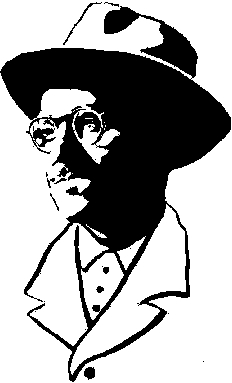
\includegraphics[width=1.5cm]{03}
\end{center}
\def\fileversion{1.004}
\def\filedate{(11-12-2022)}
{\scriptsize\squarepar{\emph{La trascendencia de lo nimio. El humor como poética en los cuentos de Efrén Hernández} de José Julián González Osorno, se terminó de componer en calle Rayón núm.~25, col. Centro, Altotonga, Veracruz (México). El ``manuscrito'' se capturó con el editor de texto plano \TeX{}maker (5.0.3) de Pascal Brachet, y se formó en el sistema de composición tipográfico \LaTeXe{} de Leslie Lamport, basado en el lenguaje de programación \TeX{} creado por \mbox{Donald E.~Knuth}; el archivo fuente fue compilado con el motor de tipografías \textsc{pdf}\TeX{} desarrollado por Hàn Th\'{ê} Thành. En su composición se utilizó tipografía Cochineal, \emph{fork} de Crimson Text de Sebastian Kosch realizado por Michael Sharpe. Las imágenes se manipularon en \textsc{gimp} (2.10.22) e Inkscape (1.0.2). Disposición tipográfica realizada para papel \emph{Bond} ahuesado tamaño carta de 90\,gr. Diseño, diagramación y composición tipográfica: \href{muxkernel@gmail.com}{Tuxkernel}. ver.\space\fileversion\space\filedate}}
\end{document}
